%% LyX 2.2.0 created this file.  For more info, see http://www.lyx.org/.
%% Do not edit unless you really know what you are doing.
\documentclass[12pt,a4paper,english,brazil]{abntex2}
\renewcommand{\familydefault}{\rmdefault}
\usepackage[T1]{fontenc}
\usepackage[utf8]{inputenc}
\setcounter{secnumdepth}{3}
\setcounter{tocdepth}{3}
\usepackage{array}
\usepackage{longtable}
\usepackage{float}
\usepackage{textcomp}
\usepackage{url}
\usepackage{pdfpages}
\usepackage{amsmath}
\usepackage{graphicx}
\usepackage[intoc]{nomencl}
% the following is useful when we have the old nomencl.sty package
\providecommand{\printnomenclature}{\printglossary}
\providecommand{\makenomenclature}{\makeglossary}
\makenomenclature

\makeatletter

%%%%%%%%%%%%%%%%%%%%%%%%%%%%%% LyX specific LaTeX commands.
\special{papersize=\the\paperwidth,\the\paperheight}

%% Because html converters don't know tabularnewline
\providecommand{\tabularnewline}{\\}
%% A simple dot to overcome graphicx limitations
\newcommand{\lyxdot}{.}


%%%%%%%%%%%%%%%%%%%%%%%%%%%%%% Textclass specific LaTeX commands.
\AtBeginDocument{                
\RequirePackage{abntex2cite}

\renewcommand{\citeauthor}[1]{\citeauthoronline{#1}}
\def\citep{\cite}
\newcommand{\citeyearpar}[1]{(\citeyear{#1})}
\ifx\AbntCitetype\AbntCitetypeALF
\def\citet{\citeonline} % alf
\newcommand{\citealt}[1]{\citeauthoronline{#1}~\citeyear{#1}}
\newcommand{\citealp}[1]{\citeauthoronline{#1},~\citeyear{#1}}
\else
\def\citet{\@ifnextchar[{\citet@with}{\citet@without}} % num
\def\citet@with[#1]#2{\citeauthoronline{#2}~\cite[#1]{#2}}
\def\citet@without#1{\citeauthoronline{#1}~\cite{#1}}
\newcommand{\citealt}[1]{\citeauthoronline{#1}~\citeonline{#1}}
\def\citealp{\citeonline}
\fi
}

%%%%%%%%%%%%%%%%%%%%%%%%%%%%%% User specified LaTeX commands.
\usepackage{indentfirst}
\usepackage{float}
\usepackage{titlesec}
\usepackage{tikz, blindtext}
\usetikzlibrary{shapes.multipart}
\usepackage{calc,soul,fourier}
\usepackage{color, colortbl}
\usepackage{graphicx}
%\usepackage[brazil]{babel}
\usepackage[brazilian,hyperpageref]{backref}
\setlength{\parindent}{48pt}
\usepackage[alf]{abntex2cite}
%\usepackage{lmodern}
\usepackage[unicode=true]{hyperref}
\hypersetup{%
pdfborder = {0 0 0},
colorlinks ,
citecolor=blue,
filecolor=blue,
linkcolor=blue,
urlcolor=blue
}


%================================================================================
%======================================
%estilo do section, subsection e subsubsection
%======================================
 
\titleformat{\section}
{\normalfont\fontsize{16pt}{18pt}\selectfont\bfseries}{\thesection}{1em}{}
\titleformat{\subsection}
{\normalfont\fontsize{14pt}{16pt}\selectfont\bfseries}{\thesubsection}{1em}{}
\titleformat{\subsubsection}
{\normalfont\fontsize{12pt}{14pt}\selectfont\bfseries}{\thesubsubsection}{1em}{}


%================================================================================
%======================================
%Pacotesdecitações
%======================================
\renewcommand*{\backref}[1]{}
\renewcommand*{\backrefalt}[4]{
\ifcase #1 (No citado.)
\or (Citado na página~#2.)
\else (Citado nas páginas #2.)
\fi%
}
\renewcommand*{\backrefsep}{, }
\renewcommand*{\backreftwosep}{e~}
\renewcommand*{\backreflastsep}{e~}
%================================================================================
% Configuração dos Estilo dos Capítulo
%================================================================================

\makechapterstyle{box}{

\renewcommand{\chapterheadstart}{}
% Secao secundaria (Section) Caixa baixa, Negrito
\renewcommand*{\cftsectionfont}{\bfseries}
% Secao terciaria (Subsection) Caixa baixa, Negrito, italico
\renewcommand*{\cftsubsectionfont}{\itshape\bfseries}
% Secao quaternaria (Subsubsection) Caixa baixa, italico
\renewcommand*{\cftsubsubsectionfont}{\itshape}
% Secao quinquenária (Subsubsubsection) Caixa baixa
\renewcommand*{\cftparagraphfont}{\normalsize}

% tamanhos de fontes de chapter e part
\ifthenelse{\equal{\ABNTEXisarticle}{true}}{%
\setlength\beforechapskip{\baselineskip}
\renewcommand{\chaptitlefont}{\ABNTEXsectionfont\ABNTEXsectionfontsize}
}{%else
\setlength{\beforechapskip}{0pt}
\renewcommand{\ABNTEXchapterfontsize}{\LARGE}
%\renewcommand{\ABNTEXchapterfont}{\sffamily\bfseries}
%alteração da fonte dos capítulos, seções e subseções
\renewcommand{\chaptitlefont}{\ABNTEXchapterfont\bfseries\ABNTEXchapterfontsize}
}
%\renewcommand{\chapter}{\chaptertitlename\ \thechapter}{0pt}{\Large\uppercase}
\renewcommand{\chapnumfont}{\chaptitlefont}
\renewcommand{\parttitlefont}{\ABNTEXpartfont\ABNTEXpartfontsize}
\renewcommand{\partnumfont}{\ABNTEXpartfont\ABNTEXpartfontsize}
\renewcommand{\partnamefont}{\ABNTEXpartfont\ABNTEXpartfontsize}

\renewcommand*{\printchaptername}{}
\renewcommand*{\chapnumfont}{\normalfont\sffamily\huge\bfseries}
\renewcommand*{\printchapternum}{
\hrulefill{\renewcommand{\arraystretch}{1.5}
\begin{tabular}{|c|}
\rowcolor{black}\color{white}\normalsize\ABNTEXchapterfont\MakeTextUppercase{\chaptername}\\
\vspace{-1.5ex}\\
\resizebox{!}{1.1cm}{\ABNTEXchapterfont\thechapter}
\\[2.5ex]
\hline
\end{tabular}
}
}

\renewcommand*{\chaptitlefont}{\normalfont\sffamily\Huge\bfseries}
\renewcommand*{\printchaptertitle}[1]{
\flushright\chaptitlefont##1
\vskip -0.6ex\hfill\rule{.8\textwidth}{0.5pt} \\
\vskip -2.8ex\hfill\rule{.8\textwidth}{2pt}\\
\vskip 1.5ex
}

}

\chapterstyle{box}

%=================================
%Configurações do estilo da pagina
%==================================

%\makepagestyle{ruled}
%\makeoddfoot{ruled}{}{}{}
%\makeevenfoot{ruled}{}{}{}
%\makeheadrule{ruled}{\textwidth}{\normalrulethickness}
%\makeevenhead{ruled}{\thepage}{}{\small\itshape\leftmark}
%\makeoddhead{ruled}{\small\itshape\rightmark}{}{\thepage}
%\makeatletter % because of \@chapapp
%\makepsmarks  {ruled}{
%\nouppercaseheads
%\createmark	{chapter} 	{both} {shownumber}{\@chapapp\ }{. \ }
%\createmark	{section} 	{right} {shownumber}{}		  {. \ }
%\createplainmark {toc}		{both}{\contentsname}
%\createplainmark {bib}		{both}{\bibname}
%}
%\makeatother
%\pagestyle{ruled}

%================================================================================
% Configuração das legendas nas figuras e tabelas
%================================================================================

\newcommand{\fautor}{\legend{Fonte: Elaborada pelo autor.}}
\newcommand{\fadaptada}[2][]{\legend{Fonte: Adaptada de \citeonline[#1]{#2}.}}
\newcommand{\fdireta}[2][]{\legend{Fonte: \citeonline[#1]{#2}.}}
\newcommand{\fdadospesquisa}{\legend{Fonte: Dados da pesquisa.}}

%\usepackage{lmodern}

%\newcommand{\blankpage}{
%\newpage
%\thispagestyle{empty}
%\mbox{}
%\newpage
%}
%\setcounter{secnumdepth}{4}

\makeatother

\usepackage{babel}
\usepackage{listings}
\addto\captionsbrazil{\renewcommand{\lstlistingname}{\inputencoding{latin9}Listagem}}
\addto\captionsbrazil{\renewcommand{\lstlistlistingname}{\inputencoding{latin9}Listagens}}
\addto\captionsenglish{\renewcommand{\lstlistingname}{\inputencoding{latin9}Listing}}
\addto\captionsenglish{\renewcommand{\lstlistlistingname}{\inputencoding{latin9}Listings}}
\renewcommand{\lstlistingname}{\inputencoding{latin9}Listagem}
\renewcommand{\lstlistlistingname}{\inputencoding{latin9}Listagens}

\begin{document}
%Configurações do estilo da pagina %==================================
\makepagestyle{ruled} 
\makeoddfoot{ruled}{}{}{}   
\makeevenfoot{ruled}{}{}{}   
\makeheadrule{ruled}{\textwidth}{\normalrulethickness}   
\makeevenhead{ruled}{\thepage}{}{\small\itshape\leftmark}   
\makeoddhead{ruled}{\small\itshape\rightmark}{}{\thepage} 
\makeatletter % because of \@chapapp      
\makepsmarks  {ruled}{  
\nouppercaseheads 
\createmark	{chapter} 	{both} {shownumber}{\@chapapp\ }{. \ } 
\createmark	{section} 	{right} {shownumber}{}		  {. \ } 
\createplainmark {toc}		{both}{\contentsname} 
\createplainmark {bib}		{both}{\bibname}}
\makeatother 
\pagestyle{ruled}

\includepdf{pages/\string"Half Title Page\string"}\clearpage{}

\includepdf{pages/\string"Title Page\string"}\clearpage{}

\includepdf{pages/\string"Title Page english\string"}\clearpage{}

\includepdf{pages/datasheet}

\clearpage{}

\includepdf{pages/Dedicatory}

\clearpage{}

\includepdf{pages/Acknowledgements}\clearpage{}
\begin{resumo}
GARAVITO, J. F. Ontologias e DSLs na geração de sistemas de apoio
à decisão, caso de estudo SustenAgro. Dissertação (Mestrado em Ciências
– Ciências de Computação e Matemática Computacional) – Instituto de
Ciências Matemáticas e de Computação, Universidade de São Paulo, São
Carlos – SP, 2017.

\vphantom{}

Os Sistemas de Apoio à Decisão (SAD\nomenclature{SAD}{Sistemas de Apoio à Decisão})
integram conhecimento dos especialistas do domínio em cada um dos
componentes deles: nos dados e modelos, nas operações matemáticas
que processam esses dados e nas informações resultantes que suportam
o processo de decisão. Nas metodologias de desenvolvimento tradicionais,
este conhecimento deve-se interpretar e implementar pelos desenvolvedores
de software, devido a que os especialistas não conseguem formalizar
esse conhecimento em um modelo computável para integrá-lo nos SADs.
Sendo realizado o processo de modelagem de conhecimento pelos desenvolvedores,
parcializando o conhecimento do domínio e dificultando o desenvolvimento
ágil dos SADs. Dada esta situação, identificou-se que não existe uma
representação de conhecimento computável que permita definir SADs,
que tenha um formato entendível e accessível pelos especialista do
domínio e pelos computadores. A partir desse problema, foram testadas
soluções, e encontrou-se que as ontologias baseadas na web semântica
representam conhecimento complexo e fornecem um formato entendível
pelos humanos e máquinas. Com o qual propôs-se o método Decisioner
de consiste em que as ontologias complementadas com \foreignlanguage{english}{Domain
Specific Language} (DSL\nomenclature{DSL}{Domain Specific Language})
permitem aos especialistas representar o conhecimento deles. Este
método foi implementado no \foreignlanguage{english}{Framework} Decisioner
que permite definir e gerar SADs em entornos web. A validação do método
foi realizada por meio da instanciação do SAD SustenAgro no Framework
Decisioner, através de uma ontologia de avaliação da sustentabilidade
em cana-de-açúcar no centro-sul do Brasil e de uma descrição na DSL,
que permitiram gerar o SAD SustenAgro. Finalmente, foram realizadas
avaliações do Framework Decisioner e do SAD SustenAgro com resultados
positivos que permitem concluir que o método proposto forneceu um
meio de representação de conhecimento do domínio para que especialistas
possam definir SADs.

\vphantom{}

\textbf{Palavras Chave:} \emph{Ontologias, Linguagem de Domínio Específico,
Web Semântica, Representação de Conhecimento, Framework Decisioner,
Sistema de apoio à decisão, SustenAgro}

\end{resumo}
\clearpage{}
\selectlanguage{english}%
\begin{resumo}
Decision Support Systems (DSS) integrate knowledge from Domain Experts
in each of their components: in data and models, in mathematical operations
that processes this data and in the resulting information that supports
the decision-making process. In traditional development methodologies,
this knowledge must be interpreted and implemented by software developers,
because the specialist can not formalize this knowledge in a computable
model to integrate it into the DSS. The knowledge modeling process
is carried out by the developers, biasing domain knowledge and hindering
the agile development of DSSs. Given this situation, it was identified
that there is no computable knowledge representation that allows define
DSSs, that has a format understandable and accessible by the domain
experts and the computers. From that problem, were tested and found
solutions based on semantic web ontologies represent complex knowledge
and provide a format understandable by human and machines. Decisioner
method allowing experts represent their knowledge by means of ontologies
and Domain Specific Languages (DSL), to allow the definition and generation
of SADs. Decisioner Framework implement this method by providing web
ontology edition interfaces and DSL to define and generate the SADs
in web environments. To validate such method, Decisioner Framework
was instantiated with an ontology of sustainability assessment in
sugarcane in the center-south of Brazil and by means of a description
in the DSL of the components of SAD, it allowed the generation the
DSS SustenAgro. Evaluations were carried out in the Framework Decisioner
and in the DSS SustenAgro to validate the proper operation of them.

\selectlanguage{brazil}%
\textbf{Palavras Chave:} \foreignlanguage{english}{Decisioner \emph{Framework,
}DSS, SustenAgro, Ontologies, Semantic Web, DSL, computable knowledge.}\selectlanguage{brazil}%


\end{resumo}
\selectlanguage{brazil}%
\clearpage{}

\listoffigures

\clearpage{}

\listoftables

\renewcommand{\lstlistlistingname}{Lista De C{\'o}digos-Fonte}

\lstlistoflistings{}

\renewcommand{\nomname}{Lista De Abreviaturas e Siglas}

\printnomenclature{}

\clearpage{}

\tableofcontents{}

\clearpage{}

\chapter{Introdução\label{chap:Introdu=0000E7=0000E3o}}

Os Sistemas de Apoio à Decisão (SAD \nomenclature{SAD}{Sistemas de Apoio à Decisão})
organizam e processam os dados e informações para gerar resultados
de valor que auxiliem o processo de decisão em um domínio especifico,
ditos sistemas integram conhecimento desenvolvido pelos especialistas
do domínio que fica implícito nos dados, informações e processos,
dito conhecimento não é familiar para os desenvolvedores de software,
o que leva a usar diversas técnicas de levantamento de requerimentos
que envolvem o aprendizado de tópicos do domínio dos especialistas
por parte dos desenvolvedores, este processo exige um esforço adicional
por parte dos desenvolvedores do sistema e traz limitações no tempo
e custo de desenvolvimento, devido a que o conhecimento precisa ser
explicado por parte dos especialistas do domínio aos desenvolvedores
de software, para que eles consigam entender o conhecimento e assim
implementar o sistema software corretamente.

Adicionalmente, os especialistas do domínio pelo geral não tem o conhecimento
de desenvolvimento de sistemas software para realizar dito processo
por eles mesmos; alem disso os dois domínios, tanto dos especialistas
do domínio como do desenvolvimento de software são tão amplos que
precisam perfis particulares para realizar os processos corretamente,
devido ao anterior foi identificado o problema da inexistência de
uma representação de conhecimento para definir SADs, que tenha um
formato computável, entendível e acessível pelos especialistas do
domínio e desenvolvedores de software.

Como exemplo do anterior problema, podermos expor o caso dos especialistas
em sustentabilidade da Embrapa Meio Ambiente, que desenvolveram o
projeto SustenAgro (capitulo \ref{chap:Sustainability_Assessment}),
onde foi desenvolvido um método de avaliação de sustentabilidade no
sistema produtivo de cana-de-açúcar, os especialistas precisavam implementar
um SAD para disponibilizar o uso do método à comunidade interessada
em realizar avaliações de sustentabilidade em cana-de-açúcar, , no
caso deles foi identificado que tinham o conhecimento do domínio avaliação
de sustentabilidade da cana-de-açúcar, mas não tinham o método e ferramenta
software para definir dito conhecimento de maneira computável em um
SAD, pelo que dito problema e caso de uso foram abordados na presente
pesquisa como projeto piloto.

\section{Motivação}

A pesquisa em representação e organização de conhecimento tem alto
impacto devido a fornece métodos e ferramentas para gerenciar o conhecimento
em diversos domínios, especificamente no desenvolvimentos dos SADs,
pode fornecer meios de integração de conhecimento que aumentam as
funcionalidades e a eficiência desses sistemas em comparação com os
métodos tradicionais de desenvolvimento.

Sobre o caso especifico do projeto SustenAgro, existem varias motivações
para desenvolver novos meios de definição de SAD, entre eles está
principalmente o fornecimento de um método e ferramenta para que os
especialistas do domínio definiam o conhecimento nos SADs, permitindo
a participação deles como descritores de conhecimento especifico,
também temos que a avaliação da sustentabilidade da cultura de cana-de-açúcar
está em continua mudança \citep{oliveira:2013}, pelo que existe a
necessidade de fornecer meios computáveis de representação desse conhecimento
que adaptem-se às mudanças do domínio e que facilite a comunicação
entre os especialistas do domínio e os desenvolvedores de software.

Além disso, permitira definir SADs com menos intervenção por parte
dos não especialistas do domínio, fazendo que a definição do conhecimento
fique em termos dos especialistas e gerenciadas por eles mesmos, fornecendo
a possibilidade de que descrevam características particulares que
requerem profundo conhecimento do domínio, finalmente fornecera aos
desenvolvedores tempo adicional para dedicar-se aos assuntos próprios
da computação, e assim agilizar o processo de desenvolvimento de SADs.

Na representação de conhecimento existem vários tipos de sistemas
de organização de conhecimento (\nomenclature{KOS}{Knowledge Organization System}
pelas siglas em inglês), um dos sistemas mais completos são as ontologias
que permitem definir, classificar, relacionar e inferir conhecimento,
e como deseja-se um meio que suporte vários aspectos do conhecimento,
se definiu usar este tipo de \foreignlanguage{english}{KOS} no processo
de modelagem, fornecendo um caso real de aprendizagem e implementação
de ontologias.

A Embrapa Meio Ambiente também tem outros SAD que podem ser avaliados
e modelados com a finalidade de desenvolver um método e ferramenta
geral de definição de SADs.

\section{Objetivo}

Desenvolver um método e ferramenta web baseados em ontologias que
permita representar o conhecimento dos especialistas do domínio para
suportar definição de SADs, e provar o funcionamento por meio da definição
do SAD SustenAgro, que tem como finalidade suportar a avaliação da
sustentabilidade nos sistemas produtivos de cana-de-açúcar no centro-sul
do Brasil 

Para atingir o objetivo proposto, foi necessário atingir os seguintes
objetivos específicos: 

\subsection*{Objetivos específicos}
\begin{itemize}
\item Desenvolver um método de definição de SAD por parte dos especialistas.
\item Definir uma arquitetura e ferramenta para definir SADs baseados em
conhecimento de domínios específicos.
\item Desenvolver uma ontologia sobre avaliação da sustentabilidade nos
sistemas produtivos de cana-de-açúcar do centro sul do Brasil, como
base conceitual e tecnológica do sistema SustenAgro.
\item Desenvolver uma ontologia sobre controles visuais para suportar a
geração da interface gráfica do SAD SustenAgro.
\item Desenvolver uma DSL que gerencie as ontologias e que flexibilize a
definição da interface de usuário por parte dos administradores do
sistema.
\item Demonstrar que o método e ferramenta de definição de SADs por parte
dos especialistas, permite a geração de sistemas funcionais.
\end{itemize}

\section{Resultados Principais}

Os principais resultados desta pesquisa e projeto de mestrado são:
\begin{itemize}
\item Método e ferramenta para definir SADs por parte dos especialistas
do domínio.
\item Ontologia sobre avaliação de sustentabilidade em cana-de-açúcar, representando
os principais conceitos desse domínio: indicadores, os índices e o
método de avaliação; permitindo assim suportar o desenvolvimento das
outras tecnologias do presente projeto.
\item Ontologia sobre interfaces gráficas que permite representar os tipos
de dados e \foreignlanguage{english}{widgets} necessários para a geração
dos Sistemas de Apoio na Decisão.
\item DSL: linguagem de domínio especifico que permite gerenciar ontologias
para definir sistemas de apoio à decisão.
\item Protótipo do Decisioner: Sistema gerador de SADs, que suporta a integração
de ontologias e DSL em ambientes web.
\item SustenAgro: Sistema de Apoio a Decisão para avaliar a sustentabilidade
em cana-de-açúcar, implementado o método SustenAgro e tecnologias
da web semântica.
\item Artigo ``\foreignlanguage{english}{Sustainability assessment of sugarcane
production systems: SustenAgro Method}'' submetido no periódico acadêmico
``\foreignlanguage{english}{Energy for sustainable Development}''
ISSN: 0973-0826 submetido na data 23 de dezembro do 2016. 
\end{itemize}

\section{Organização}

Este trabalho de dissertação está estruturado da seguinte forma: 

Capítulo 2: Apresenta o SAD SustenAgro e os trabalhos relacionados
sobre geração de Sistemas de Apoio à Decisão e os Sistemas de Avaliação
da Sustentabilidade para representar o estado da arte da presente
pesquisa.

Capítulo 3: Apresenta a fundamentação teórica sobre Ontologias e DSL
com a finalidade de descrever as principais tecnologias e a teoria
necessária para desenvolver o presente trabalho.

Capítulo 4: Apresenta o protótipo do sistema Decisioner que permite
suportar a geração de Sistemas de Apoio à Decisão. 

Capítulo 5: Apresenta o SAD SustenAgro, desenvolvido na presente pesquisa
e que se serviu como primeiro caso de uso do sistema Decisioner, para
definir a arquitetura dele e demostra a funcionalidade do sistema
desenvolvido.

Capítulo 6: Apresenta a avaliação realizada pelos especialistas.

Capítulo 7: Apresenta as conclusões do presente trabalho, uma discussão
e possíveis trabalhos futuros.

Finalmente são apresentados os anexos que descrevem conceitos específicos
do trabalho.


\chapter{SAD\label{chap:SAD}}

A construção de sistemas que sejam capazes de fornecer suporte ao
gestor em um processo de tomada de decisões tem sido um desafio ao
longo dos anos. A continuação será explicado a definição e arquitetura
de SAD, o SAD SustenAgro e os trabalhos relacionados.

\section{Definição de SAD}

Os Sistemas de Apoio à Decisão (SAD) são uma área de conhecimento
ampla e em continua evolução. A definição de SAD deriva da definição
de sistema, pois eles contêm um conjunto de partes organizadas para
um proposito comum, existem múltiplas definições do termo SAD, a continuação
serão apresentadas algumas definições que permitem explicar o proposito
deste tipo de sistemas.

\citet{Tweedale2016} define os SADs como sistemas software que visam
melhorar a tomada de decisão individual ou grupal, combinando o conhecimento
do(s) tomador(es) de decisão com dados relevantes de fontes confiáveis,
nos quais são aplicados métodos e modelos matemáticos para suportar
a análise, comparação e escolha de alternativas no processo de decisão.

\citet{heinzle2010semantica} define que os SADs apoiam o entendimento
de processos complexos, auxiliam na comparação dos fenômenos envolvidos
e suportam a análise e escolha de alternativas no processo de decisão.
Este entendimento do domínio surge da combinação das habilidades e
metodologias dos especialistas (humanos) à capacidade dos computadores
de acessar dados, estruturá-los em modelos, interpretar, formular
e avaliar alternativas e cenários distintos.

O conhecimento dos especialistas do domínio está implícito nos SADs.
\citet{Evans:2003:DDT:861502} explica que existe uma necessidade
de modelar o conhecimento chave de um domínio em um modelo, para permitir
a comunicação e colaboração entre especialistas de domínio e os desenvolvedores,
pelo qual o modelo de conhecimento dos especialistas será objeto da
pesquisa. O processo de modelagem pode ser lento e custoso, já que
os dois grupos de profissionais têm \foreignlanguage{english}{\emph{Backgrounds}}
diferentes, que dificultaram o processo de desenvolvimento e testes
de um SAD.

Os especialistas de domínio e os desenvolvedores, pelo geral são de
organizações diferentes, o que dificulta ainda mais o processo, pelo
qual foram pesquisados modelos que facilitem o entendimento entre
os dois tipos de profissionais e desenvolvida uma pesquisa ao redor
deste tópico.

A continuação será apresentada a arquitetura dos SAD e a importância
dos modelos de conhecimento existentes dentro um SAD. 

\section{Arquitetura para Sistemas de Apoio à Decisão}

A arquitetura de um software define a organização dele em termos de
componentes, de interconexões, e das interações com sistemas externos
\citep{de1997software}. A arquitetura fornece as informações de como
os componentes dela se relacionam, explicando a parte externa das
ligações entre seus elementos, sendo que as implementações internas
não são consideradas parte da arquitetura \citep{sei2006architecture}.

Estas partes são descritas por meio da arquitetura representada na
figura \ref{fig:Componentes-SAD}, representando o processo realizado
pelos SADs, no qual recebem uma entrada, fazem o processamento dela
e retorna resultados que são analisadas pelo tomador(es) de decisão
a través da tecnologia computacional \citep{Tweedale2016}. 

\begin{figure}[H]
\noindent \begin{centering}
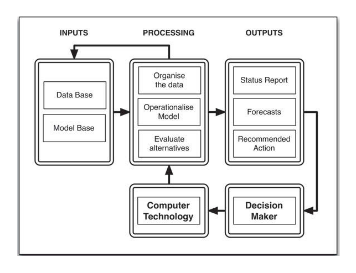
\includegraphics[width=0.8\columnwidth]{figures/DSS}
\par\end{centering}
\caption{Componentes de um SAD.\label{fig:Componentes-SAD} }

\fadaptada{Tweedale2016}
\end{figure}

A Figura \ref{fig:Componentes-SAD} mostra os componentes de um SAD,
que são: 
\begin{description}
\item [{I\foreignlanguage{english}{nputs}}] corresponde às entradas do
sistema, composta dos dados que serão processados e dos modelos de
conhecimento dos especialistas. Os dados estão armazenados em bancos
de dados e os modelos pelo geral estão implícitos no SAD ou podem
estar em uma base de conhecimento. Esses dois componentes devem ser
o mais precisos e completos possíveis para garantir respostas confiáveis
do sistema.
\selectlanguage{english}%
\item [{Processing}] \foreignlanguage{brazil}{está composto pelos modelos
e métodos de organização e processamento dos dados, que tem restrições
para avaliar as alternativas de resposta. Os métodos podem ser de
tipo matemáticos, que processam os dados e geram os resultados do
sistema.}
\item [{Outputs}] \foreignlanguage{brazil}{são os resultados do processamento
dos inputs e permitem comparar as alternativas de decisão. As saídas
comuns são relatórios, previsões e recomendações, que são apresentados
por meio de uma interface de usuário para facilitar o entendimento
e interação por parte dos usuários.}
\end{description}
Durante a evolução dos SAD, várias melhorias aconteceram, entre elas
o desenvolvimento da Web permitiu integrar novas técnicas no processamento
dos dados, tecnologias na representação visual de resultados e no
uso colaborativo por parte dos usuários \citep{Shim2002}. Também
existe a tendência da integração com métodos de inteligência artificial,
para estender a aplicabilidade dos SAD a problemas complexos. 

Uma variação dos SADs integra bases de conhecimento que suportam inferência,
permitindo o desenvolvimento de \foreignlanguage{english}{Expert Systems}
e \foreignlanguage{english}{Knowledge Based Systems.} Esses sistemas
são classificados como \foreignlanguage{english}{Rule Based Systems}
\citep{Tweedale2016}, os quais estabelecem o escopo desta pesquisa. 

Um tipo de SAD que usa bases de conhecimento, são os que usam ontologias
para representar o conhecimento dos especialistas, permitindo definir,
classificar, relacionar e inferir conhecimento. 

A continuação será apresentado o SAD SustenAgro baseado em conhecimento,
que suporta a avaliação da sustentabilidade em cana-de-açúcar a través
do uso de ontologias.

\section{SAD SustenAgro\label{sec:SAD-SustenAgro}}

Um domínio de conhecimento caracterizado pela sua complexidade são
os sistemas produtivos agrícolas. Eles envolvem fenômenos de natureza
diversa \citep{simon1991architecture}, integrando aspectos ambientais,
sociais e econômicos.

Particularmente, o setor produtivo produtivo da cana-de-açúcar é extremamente
importante para a economia do estado de São Paulo e do Brasil, devido
ao fato de ser uma das principais culturas produzidas no país \citep{Storquato2015}.
Atualmente a cana-de-açúcar é a mais importante fonte de energia renovável
no Brasil \citep{seabra2011life}, permitindo a produção de etanol
e energia eléctrica, além de ter mais de 20 subprodutos, entre eles
açúcar, etanol, bioeletricidade, bioplásticos e Hidrocarbonetos \footnote{\url{http://sugarcane.org/sugarcane-products}}. 

A produção da cana-de-açúcar e dos subprodutos dela, influem em aspectos
ambientais consumindo recursos naturais, em aspectos sociais envolvendo
pessoas na produção e em aspectos econômicos na comercialização. Esses
aspectos fazem complexo manter a produtividade atualmente e no futuro.
Por essas razões, a Embrapa Meio Ambiente escolheu especificamente
o sistema produtivo da cultura de cana-de-açúcar na região centro-sul
do Brasil, como sistema piloto para desenvolver métodos e software
de avaliação da sustentabilidade (apêndice \ref{chap:Sustainability_Assessment}).

Dada a complexidade da análise da sustentabilidade em sistemas de
produção agrícola, os pesquisadores da Embrapa Meio Ambiente trabalharam
na definição de métodos que permitissem avaliar a sustentabilidade
de maneira integral \citep{Singh2012281}. Por essa razão, desenvolveram
um método que aborda a avaliação em termos de indicadores, simplificando
a complexidade deste sistema agrícola. Cada indicador mede um determinado
aspecto crítico no sistema produtivo, para determinar o quão sustentável
ele é. A partir da análise de cada indicador, é possível gerar recomendações
de medidas corretivas para as unidades produtivas ou para o embasamento
de políticas públicas que incentivem a sustentabilidade. A definição
conceitual do processo de avaliação está detalhada no apêndice \ref{chap:Sustainability_Assessment}. 

A partir do método de avaliação SustenAgro, foi desenvolvida uma ferramenta
de avaliação da sustentabilidade intitulada SAD SustenAgro que implementa
o método SustenAgro por meio de um sistema de apoio a decisão e que
consegue adaptar-se às mudanças do domínio.

O SAD SustenAgro suporta a avaliação da sustentabilidade em cana-de-açúcar
no centro-sul do Brasil. A figura \ref{fig:SustenAgro-arquitetura-inicial}
apresenta a arquitetura inicial do SAD SustenAgro, a qual corresponde
a um sistema de informação tradicional, que requer a intervenção de
desenvolvedores de software, para definir ou atualizar o conhecimento
dos especialistas implícito no SAD.

\begin{figure}[h]
\begin{centering}
\includegraphics[width=0.6\columnwidth]{\string"figures/SustenAgro Initial Architecture\string".eps}
\par\end{centering}
\caption{SustenAgro arquitetura inicial.\label{fig:SustenAgro-arquitetura-inicial}}
\end{figure}

Os especialistas em sustentabilidade definiram o SAD Sustenagro com
as seguintes características:
\begin{itemize}
\item Sistema web com banco de dados para armazenar e recuperar as informações
do sistema.
\item Integração e implementação do método SustenAgro de avaliação de sustentabilidade,
descrito no apêndice \ref{chap:Sustainability_Assessment} 
\item Flexibilidade para adaptar o método SustenAgro a outras culturas.
\item Integração com sistemas de georreferenciamento.
\item Desenvolvimento de \foreignlanguage{english}{widgets} especificas
\footnote{\selectlanguage{english}%
Widgets\foreignlanguage{brazil}{ refere-se à componentes visuais dos
sistemas web }\selectlanguage{brazil}%
} para mostrar resultados obtidos: \foreignlanguage{english}{Sustainability
Matrix }e \foreignlanguage{english}{Sustainability Semaphore,} explicadas
no capítulo \foreignlanguage{english}{\ref{chap:SustenAgro}}
\item Geração de relatórios e de recomendações de sustentabilidade.
\end{itemize}
Um dos problemas identificados foi que os especialistas não tinham
uma definição clara do SAD SustenAgro. Pelo que foi necessário realizar
um levantamento de requisitos, descrito no capítulo \ref{chap:SustenAgro},
para definir os requisitos funcionais (essenciais) e não funcionais
(desejáveis). Além disso, foi necessário reestruturar o desenvolvimento
do SAD SustenAgro para que fizesse parte do processo de pesquisa.

O SAD SustenAgro faz parte de um conjunto de ferramentas de avaliação
definidas pela Embrapa Meio Ambiente. A partir do analise das ferramentas
similares ao SAD SustenAgro, foi evidenciada a necessidade de fornecer
métodos e ferramentas computacionais que organizem a informação. Para
apoiar aos especialistas a tomar decisões baseadas em conhecimento,
permitindo simplificar a resolução de problemas que de outra maneira
não seriam triviais. 

Exatamente foi identificado que ditos sistemas tinham em comum um
método de avaliação que processava de maneira matemática um conjunto
de dados e gerava relatórios com resultados da avaliação, gráficos
e recomendações. As ferramentas analisadas foram:
\begin{enumerate}
\item Sistema Innova-Tec: avaliação do impacto da inovação tecnológica\footnote{\url{http://www.cnpma.embrapa.br/forms/inova_tec.php3}}.
\item Sistema Nano-Tec: avaliação do impacto das nanotecnologias\footnote{\url{https://www.embrapa.br/en/busca-de-publicacoes/-/publicacao/951543/metodologia-para-avaliacao-de-impactos-das-nanotecnologias-metodo-e-software-impactos-nanotec} }.
\item Sistema GMP-RAM v.1.1: avaliação de Risco de Plantas Geneticamente
Modificadas (GMP \nomenclature{GMP}{Genetically Modified Plants})\footnote{\url{http://www.cnpma.embrapa.br/forms/gmp_ram.php3}}
\item Software para avaliação de segurança e impactos de plantas geneticamente
modificadas\footnote{\url{http://www.cnpma.embrapa.br/nova/mostra2.php3?id=857}}
\item Sistema Atlantis: Sistema para levantamento e sistematização da informação
técnica em temas de pesquisa, tecnologias e inovação. \footnote{\url{https://www.embrapa.br/en/busca-de-produtos-processos-e-servicos/-/produto-servico/2102/atlantis---atlantis}}
\end{enumerate}
Uma característica importante em ditos sistemas foi a existência de
conceitos de domínio especifico na organização dos dados de entrada
dos SAD e no método de avaliação. Esta característica permite identificar
que cada um dos sistemas requiriu um processo de modelagem dos conceitos
do domínio por parte dos desenvolvedores. 

Principalmente identificou-se que a implementação desse conhecimento
gerava dificuldades de compreensão entre os especialistas do domínio
e os desenvolvedores de software por serem de áreas diferentes. \citet{Evans:2003:DDT:861502},
propõe que este conhecimento deve ser representado em um modelo independente.

Baseando-se no anterior, afirmou-se a hipótese de usar um modelo para
representar dito conhecimento. E baseando-se no problema de pesquisa,
as ontologias foram selecionadas como o modelo mais completo para
representar o conhecimento do domínio dos especialistas na definição
de SAD, e evitar que o conhecimento ficara implícito como aconteceu
nos SAD listados.

O uso de uma ontologia permitirá representar e estruturar o conhecimento
de avaliação da sustentabilidade em agricultura, a través da definição
e atualização de conceitos por parte dos especialistas, permitindo
que eles mesmos descrevam o domínio sem precisar dos desenvolvedores.
Os especialistas do domínio tem familiaridade com os termos da ontologia
e poderão especificar grande parte do conhecimento envolvido no SAD.
Idealmente, essa definição deve ser detalhada o suficiente para que
os desenvolvedores possam desenvolver a parte computacional do SAD
sem necessidade de \foreignlanguage{english}{feedback} dos especialistas.

Esta representação de conhecimento pode ser mais exata da realidade
do que outros modelos, devido a que está em um formato voltado a descrição
de conhecimento, sobre o qual é possível fazer inferências e assim
gerar informações para suportar a decisão. A partir dessa definição
computável será gerado o SAD SustenAgro. 

Devido a este contexto, o SAD SustenAgro foi escolhido como projeto
piloto para desenvolver a presente pesquisa, porque permite o desenvolvimento
de um SAD baseado em conhecimento e que permite explorar alternativas
na definição e geração dos SAD.

\section{Trabalhos relacionados}

Com a finalidade de relacionar pesquisas sobre o tema que forneçam
ideias e exemplos para abordar o problema, realizou-se uma consulta
na literatura por SADs que usassem ontologias do domínio dos especialistas,
e SADs semelhantes ao SustenAgro. Foi feita uma pesquisa bibliográfica
utilizando fontes de informação acadêmica.

Sobre o uso de ontologias em domínios similares ao SustenAgro:

O vocabulário\emph{ }\foreignlanguage{english}{\emph{Agricultural
Vocabulary (AGROVOC\nomenclature{AGROVOC}{Agricultural vocabulary})}}
\footnote{Definição do Agrovoc\url{http://aims.fao.org/agrovoc}}
que é um \foreignlanguage{english}{\emph{thesaurus}} (sistema de referência
de termos) fornece termos padronizados sobre alimentação, nutrição,
agricultura, pesca, floresta e meio ambiente criados de maneira colaborativa
e coordenados pela \foreignlanguage{english}{\emph{Food and Agricultural
Organization}}\emph{ }\footnote{\emph{Site da FAO \url{http://www.fao.org/home/en/}}}\emph{(FAO}). 

Esses termos podem ser reutilizados em ontologias \citep{DCMIPro841},
permitindo uma padronização com os identificadores dos conceitos,
reutilizando informações e integrando os conceitos com outros dados
da \foreignlanguage{english}{Linked Open Data} (\foreignlanguage{english}{LOD}\nomenclature{LOD}{Linked Open Data})

\citet{kraines2011system} desenvolveram uma ferramenta com o objetivo
de criar um sistema de compartilhamento de conhecimento (\foreignlanguage{english}{\emph{Knowledge
Sharing System}}), para a ciência da sustentabilidade, por meio de
um processo de modelagem semântica. Uma ontologia, fundamentada em
lógica descritiva, foi desenvolvida por meio do modelo de dados ISO
15926 para descrever três tipos de conceitualizações de ciência sustentável:
conhecimento situacional, métodos analíticos e \foreignlanguage{english}{frameworks}
de cenários. Os conhecimentos dos especialistas podem ser descritos
por meio de afirmações semânticas (\foreignlanguage{english}{\emph{semantic
statements}}). Utilizando a ontologia, foram usados o \foreignlanguage{english}{\emph{matching}}
semântico, baseado em lógica, e inferência, baseada em regras, para
quantificar a sobreposição conceitual das afirmações semânticas.

Cada uma dessas pesquisas fornece um exemplo do uso de ontologias
na criação de soluções baseadas em conhecimento. Isto foi confirmado
por \citep{roussey2010ontologies} que afirma que o uso ontologias
têm sido realizado em várias aplicações relacionadas a agricultura.
Dadas as afirmações dessas pesquisas, pode-se concluir que uma ontologia
pode proporcionar o suporte na representação e organização de conhecimento
necessário para cumprir os requisitos do sistema SustenAgro.

Sobre a busca de SADs semelhantes ao SustenAgro, encontrou-se: 

Uma estratégia para abordar a complexidade em SADs é a utilização
de métodos e metodologias de avaliação que utilizam indicadores, um
exemplo desse enfoque é a pesquisa de \citet{AlkanOlsson:2009}. Nela
foi desenvolvido um \foreignlanguage{english}{\emph{framework}} de
indicadores que relaciona, de uma maneira consistente, as dimensões
ambiental, econômica e social do desenvolvimento sustentável. Seu
principal benefício é uma relativa simplicidade na apresentação da
informação e a possibilidade de vincular novos indicadores.

\citet{Ewert2009546} apresentam várias estratégias para abordar a
complexidade nos sistemas agrícolas. Eles começam relacionando a agricultura
com os sistemas socioeconômicos e naturais e enfrentam o problema
de gerir suas múltiplas funções, de uma maneira sustentável.

Existem pesquisas que abordam a sustentabilidade através de ferramentas
tecnológicas, as quais podem servir de referência ao sistema SustenAgro.
Uma delas foi desenvolvida por \citep{brilhante:2006} e consiste
em um \emph{framework} (MOeMA-IS) para análise de aspectos de sustentabilidade
do estado do Amazonas. Ele usa uma ontologia para descrição de indicadores
de sustentabilidade (\foreignlanguage{english}{ISD-Economics Ontology}).
Foram utilizados indicadores classificados em humanos (Social), suporte
(Econômico) e naturais (Ambiental), que foram subdivididos em sete
indicadores. Seu desenvolvimento foi feito de uma maneira genérica
de forma que ela suporta a inclusão de novos indicadores de forma
simples. 


\section{Considerações finais}

 O desenvolvimento do SAD SustenAgro, permite avaliar se as ontologias
fornecem o suporte de representação de conhecimento para definir o
conhecimento do domínio e testar novas possibilidades na definição
e geração de SAD baseados em conhecimento.

Desta forma tentar solucionar o problema da inexistência de uma representação
de conhecimento para definir SADs, que tenha um formato computável,
entendível e acessível aos especialistas do domínio e desenvolvedores
de software.


\chapter{Web Semântica e \foreignlanguage{english}{DSLs}\label{chap:SemanticWebAndDSLs}}

Ontologias da web semântica e \foreignlanguage{english}{DSLs} têm
um papel fundamental na criação de um meio de descrição de conhecimento
por parte dos especialistas e portanto suportar o design de SADs baseados
em conhecimento. 

Ontologias servem para representar o conhecimento de especialistas
do domínio e DSLs servem para customizar o comportamento dos SADs.
As ontologias apareceram originalmente no contexto da filosofia, onde
se referem ao estudo da natureza, existência e realidade dos entes.
Elas são usadas em vários campos do conhecimento. Neste projeto, ontologias
referem-se a representações de conhecimento, que precisam ser implementadas
em código. As implementações de software podem trabalhar com ontologias
da Web Semântica que fornecem a criação, armazenamento, busca e modificação
de ontologias, seguindo padrões de formatos abertos. 

Neste capítulo, vamos apresentar e discutir as ontologias da web semântica
e as DSLs. Descrevendo a teoria da Web Semântica: fundamentos, Ontologias,
o \foreignlanguage{english}{Resource Description Framework (RDF}\nomenclature{RDF}{Resource Description Framework})
e a \foreignlanguage{english}{Web Ontology Language} (\foreignlanguage{english}{OWL}\nomenclature{OWL}{Web Ontology Language}).
Finalmente serão abordadas as \foreignlanguage{english}{Domain Specific
Languages (DSLs}) que são linguagens que permitem definir um meio
de comunicação entre os especialistas e o sistema desenvolvido.

\section{Web Semântica.}

A web foi criada para possibilitar o acesso, intercâmbio e recuperação
de informações de maneira rápida e simples, seu crescimento exponencial
e caótico fez com que a mesma se tornasse hoje um gigantesco repositório
de documentos, o que dificulta a recuperação de informações. Até o
momento, não existe nenhuma estratégia abrangente e satisfatória para
a organização de documentos por meio de “motores de busca” que seja
coerente com uma estrutura linguística. \citep{Souza:2004}.

Um exemplo da deficiência da web atual, pode ser identificada na busca
realizada pelos sistemas de recuperação de informação, que usam palavras-chave
nas buscas, onde apenas a similaridade e o número de ocorrências de
certas palavras no conteúdo de documentos são levados em consideração
e não a semântica presente naquela informação. \citep{Souza:2004}.

A Web Semântica aparece como uma proposta para organizar o conhecimento
da internet semanticamente em formatos entendíveis pelos humanos e
máquinas \citep{bernerslee2001}. Procurando métodos para que as máquinas
consigam realizar a interpretação do significado, que é uma habilidade
inata dos seres humanos, através da associação dos conceitos que estão
no cérebro por meio de estruturas neurais e que não é suportado pelas
máquinas tradicionais.

A Web Semântica tem como finalidade estruturar os dados e informações
disponíveis na Web, para que tenham significado e sejam computáveis
por máquinas. Gerando um ambiente onde agentes de software e usuários
possam trabalhar de maneira cooperativa. A Web Semântica é definida
por um conjunto de padrões propostos pelo \foreignlanguage{english}{World
Wide Web Consortium} (W3C \nomenclature{W3C}{World Wide Web Consortium}).
A figura \ref{fig:Semantic_Web_History} apresenta alguns dos padrões
que constituem a Web Semântica de maneira cronológica.

\begin{figure}[H]
\begin{centering}
\includegraphics[width=1\columnwidth]{\string"figures/Semantic Web History\string".eps}
\par\end{centering}
\caption{História da Web Semântica \label{fig:Semantic_Web_History}}

\fadaptada{bikakis2013xml}
\end{figure}

\citet{bernerslee2001} propuseram a Web Semântica, em 2001, como
uma extensão da Web atual, na qual é possível vincular conceitos de
maneira estruturada e padronizada. Permitindo a criação de conhecimento
estruturado, computável por máquinas, que pode ser compartilhado entre
humanos e máquinas. A finalidade é criar uma web universal dos conhecimentos
da humanidade. 

A partir dessa visão conceitual sobre a Web, \citet{bernerslee2001}
propuseram uma arquitetura que organiza as representações do conhecimento
por meio de camadas, conhecida como \foreignlanguage{english}{Semantic
Web Cake,} que é ilustrada na Figura \ref{fig:Web-Semantic-Architecture}.

\begin{figure}[H]
\begin{centering}
\includegraphics[width=0.6\columnwidth]{\string"figures/Semantic Web Architecture\string".eps}\caption{Arquitetura em camadas da Web Semântica\label{fig:Web-Semantic-Architecture}}
\par\end{centering}
\fadaptada{fensel2011semantic}
\end{figure}

A base dessa arquitetura é estabelecida pelos padrões \foreignlanguage{english}{Unicode}
e \foreignlanguage{english}{Uniform Resource Identifier} (URI\nomenclature{URI}{Uniform Resource Identifier}),
que padronizam a representação dos dados por meio das seguintes camadas: 
\selectlanguage{english}%
\begin{description}
\item [{Unicode}] \foreignlanguage{brazil}{é um padrão que codifica os
caracteres na maioria dos sistemas de escrita para representação de
texto com fines de processamento computacional.}
\item [{URI}] \foreignlanguage{brazil}{permite identificar os recursos
disponíveis na Web por meio de uma }String\foreignlanguage{brazil}{
única.}
\item [{XML\foreignlanguage{brazil}{\nomenclature{XML}{Extensible Markup Language}}}] \foreignlanguage{brazil}{representa
os dados de maneira sintática, através da definição de }markups\foreignlanguage{brazil}{
que codificam documentos em formatos preestabelecidos. Ela permite
que informações sejam legíveis tanto por humanos como por computadores,
suportando as camadas superiores na arquitetura.}
\item [{RDF}] \foreignlanguage{brazil}{é um modelo padrão para intercambiar
dados na web. }RDF\foreignlanguage{brazil}{ tem características que
permitem a integração de dados inclusive de esquemas diferentes, e
suporta especialmente a evolução dos esquemas através do tempo sem
requerer que mudanças nos consumidores de dados. RDF é uma recomendação
do W3C}\footnote{\selectlanguage{brazil}%
\url{https://www.w3.org/RDF/}\selectlanguage{brazil}%
}\foreignlanguage{brazil}{.}
\item [{Ontology}] \foreignlanguage{brazil}{estende a camada de descrição,
fornecendo mais expressividade na definição de conceitos, de classificações,
de relações e de inferência.}
\item [{Logic}] \foreignlanguage{brazil}{permite definir regras lógicas
para deduzir e inferir novas informações que conseguem mudar a estrutura
da ontologia de maneira dinâmica.}
\item [{Proof}] \foreignlanguage{brazil}{fornece mecanismos para avaliar
o nível de confiabilidade das fontes de recursos e informações.}
\item [{Trust}] \foreignlanguage{brazil}{representa o conhecimento validado
e confiável.}
\item [{Digital-Signature}] \foreignlanguage{brazil}{permite integrar métodos
de segurança que garantam a segurança da informação.}
\end{description}
\selectlanguage{brazil}%
Uma das contribuições importantes da Web Semântica foi a formalização
da representação de ontologias (próxima sessão). No desenvolvimento
desta pesquisa, foram usadas desde as camadas inferiores até o \foreignlanguage{english}{OWL},
permitindo definir ontologias que representam os domínios de conhecimento.

\subsection*{Ontologias}

Existem várias interpretações do conceito ontologia, dependendo da
finalidade para qual elas sejam usadas. \citet{Smith2007} descrevem
a ontologia como uma área da filosofia, que estuda a natureza, existência
e realidade dos entes, assim como as categorias do ser e das relações
semânticas.

Na ciências da computação e informação, a palavra ``ontologia''
é definida como uma especificação formal e explicita de uma conceitualização
compartilhada de um domínio de conhecimento. \citet{allemang2011semantic}
definem as ontologias, no contexto da Web Semântica, como um esquema
de representação que permite conceitualizar e estruturar conhecimento,
permitindo a sua interpretação por computadores, com o objetivo de
compartilhar conhecimento entre humanos e computadores.

Uma ontologia é um sistema de organização e representação do conhecimento,
do inglês \foreignlanguage{english}{Knowledge Organization System
(KOS)}, que é uma estrutura conceitual e computacional que permite
representar o conhecimento, de qualquer domínio, por meio de entidades,
classificações, relações semânticas, regras e axiomas. Uma ontologia
é especificada por meio de componentes básicos que são as classes,
relações, axiomas e instâncias. 
\begin{description}
\item [{Classes}] são o foco da maioria das ontologias. Elas são utilizadas
para descrever os conceitos de um domínio, possibilitando a organização
e classificação dos indivíduos em um sistema lógico e hierárquico,
contendo subclasses que representam conceitos específicos \citep{noy2001ontology}. 
\item [{Relações}] representam o tipo de interação entre os conceitos de
um domínio e as propriedades presentes nas classes e indivíduos. Elas
podem ter características próprias, como serem transitivas, simétricas,
ou terem uma cardinalidade definida. 
\item [{Axiomas}] são utilizados para modelar regras assumidas como verdadeiras
no domínio em questão, de modo que seja possível associar relacionamentos
entre os indivíduos, além de fornecer características descritivas
e lógicas para os conceitos. 
\item [{Indivíduos,}] ou instâncias das classes, são utilizados para representar
elementos específicos, ou seja, os próprios dados, que juntamente
com a definição de uma ontologia, constituem a base de conhecimento
\citep{noy2001ontology}. Indivíduos representam objetos do domínio
de interesse \citep{horridge2011owl}.
\end{description}
Segundo \citet{Patel-schneider05buildingthe}, a representação de
uma ontologia é feita por meio de lógica de predicados e lógica descritiva,
usando padrões adotados pela comunidade, como \foreignlanguage{english}{RDF}
e \foreignlanguage{english}{OWL}. A Figura \ref{fig:Smart-data-continuum}
mostra os níveis de representação de dados na forma de conhecimento
processável por máquinas.

\begin{figure}[H]
\begin{centering}
\includegraphics[width=0.6\columnwidth]{\string"figures/smart data\string".eps}\caption{\foreignlanguage{english}{Smart data continuum\foreignlanguage{brazil}{: níveis de representação
de dados na forma de conhecimento processável por máquinas.\label{fig:Smart-data-continuum}}}}
\par\end{centering}
\fadaptada{allemang2011semantic}
\end{figure}

O nível mais baixo de representação começa com os dados sem nenhum
significado semântico, dependentes do contexto da aplicação. O segundo
nível envolve a definição de esquemas \foreignlanguage{english}{XML}
para conseguir independência dos dados da aplicação, os dados fluem
entre aplicações em um único domínio mas não podem ser compartilhados
fora do domínio. No terceiro nível, os dados podem ser combinados
a partir de diferentes domínios, sendo suficientemente independentes
para serem recuperados e combinados com outras fontes de dados. Finalmente
no quarto nível, é possível inferir novos dados a partir dos existentes
e compartilhá-los entre aplicações sem requerer interferência humana
\citep{sugumaran2011}.
\selectlanguage{english}%

\subsection*{Resource Description Framework\foreignlanguage{brazil}{ (}RDF\foreignlanguage{brazil}{)}}

\selectlanguage{brazil}%
O \foreignlanguage{english}{Resource Description Framework (RDF)}
é uma família de especificações da W3C, que foi disponibilizada em
1999 como parte do W3C's \foreignlanguage{english}{Semantic Web Effort}.
Elas fornecem um \foreignlanguage{english}{framework} comum que permite
que dados sejam compartilhados e reusados através das fronteiras das
aplicações, empresas e comunidades \footnote{\url{http://www.w3.org/2001/sw/}}.
O \foreignlanguage{english}{RDF} foi originalmente projetado como
um modelo de metadados e também chegou a ser usado como um método
de descrições conceituais, principalmente para descrever recursos
web e formalmente é um formato de dados de tipo grafo direcionado
e rotulado para representar informação na web\footnote{\url{https://www.w3.org/TR/rdf-sparql-query/}}.

O \foreignlanguage{english}{RDF} é usado em várias áreas de aplicação,
como \foreignlanguage{english}{\emph{resource discovery}}, para melhorar
as capacidades dos motores de busca, \foreignlanguage{english}{\emph{cataloging}},
para descrever conteúdo e as relações de conteúdo disponibilizados
em um sistema web particular, e descrição de \foreignlanguage{english}{\emph{intellectual
property rights}} de páginas web. Seu modelo básico de dados consiste
em um padrão de três tipos de objetos, conhecido como triplas\label{triplas}:
\begin{itemize}
\item \textbf{Sujeito}: representa os recursos e são identificados por meio
de \foreignlanguage{english}{URIs}. Por exemplo, uma página web ou
um elemento \foreignlanguage{english}{HyperText Markup Language (HTML
\nomenclature{HTML}{HyperText Markup Language})} podem ser recursos.
\item \textbf{Predicado}: são aspectos, características, atributos ou relações
especificas que descrevem o sujeito, cada predicado têm um significado
especifico e relaciona um sujeito com um objeto.
\item \textbf{Objeto}: um recurso especifico ou valor de propriedade que
representa uma características do sujeito \footnote{http://www.w3.org/TR/PR-rdf-syntax/}
\end{itemize}
Com \foreignlanguage{english}{RDF} é possível explicitar relações
entre dois objetos (usando-se uma Tripla \foreignlanguage{english}{RDF}),
mas não é possível fazer modelagens especificas nem inferência. Para
descrever detalhadamente o que um objeto representa e suas relações
com outros objetos, são necessárias ontologias descritas no padrão
\foreignlanguage{english}{OWL}. 
\selectlanguage{english}%

\subsection*{SPARQL Protocol and RDF Query Language (SPARQL\nomenclature{SPARQL}{SPARQL Protocol and RDF Query Language})}

SPARQL\foreignlanguage{brazil}{ é uma linguagem de consulta semântica
usada por bancos de armazenamento e recuperação de dados de dados
compatíveis com o formato }RDF\foreignlanguage{brazil}{ ou que sejam
fornecidos como }RDF\foreignlanguage{brazil}{ via }middleware\foreignlanguage{brazil}{.
Atualmente é um padrão especificado pela }W3C\foreignlanguage{brazil}{
e uma das tecnologias principais da web semântica.}

\selectlanguage{brazil}%
A versão de SPARQL 1.1, veio com novas características que permitem
a atualização de dados em formato \foreignlanguage{english}{RDF},
permitindo atualizar, criar e remover dados em formato \foreignlanguage{english}{RDF}
em um \foreignlanguage{english}{Graph Store}\footnote{\url{https://www.w3.org/TR/sparql11-update/}}.
\selectlanguage{english}%

\subsection*{Web Ontology Language\foreignlanguage{brazil}{ (}OWL\foreignlanguage{brazil}{)}}

\selectlanguage{brazil}%
A \foreignlanguage{english}{Web Ontology Language} (\foreignlanguage{english}{OWL})
foi recomendada pelo W3C em 2004 para representar e compartilhar ontologias
na Web. Essa linguagem foi projetada para aplicações que necessitam
processar o conteúdo da informação, em vez de apenas organizar informações
em nós \citep{mcguinness2004owl}. \foreignlanguage{english}{OWL}
é uma linguagem que permite que a semântica seja explicitamente associada
ao conteúdo dos dados na web e formalmente especificada através de
ontologias, compartilhadas na Internet. 

A versão \foreignlanguage{english}{OWL} 2 é a versão mais recente
da linguagem. De acordo com as especificações do W3C\footnote{http://www.w3.org/TR/owl2-overview/},
a \foreignlanguage{english}{OWL 2} adicionou três novos perfis (\foreignlanguage{english}{sub-linguagens})
aos perfis DL e \foreignlanguage{english}{Full} já existentes: \foreignlanguage{english}{OWL
2} EL,\foreignlanguage{english}{ OWL 2 QL} e \foreignlanguage{english}{OWL
RL} (Figura \ref{fig:OWL2-Profiles}). Cada um desses perfis fornece
características de expressividade diferente para diversos cenários
de aplicação:

\begin{figure}[H]
\begin{centering}
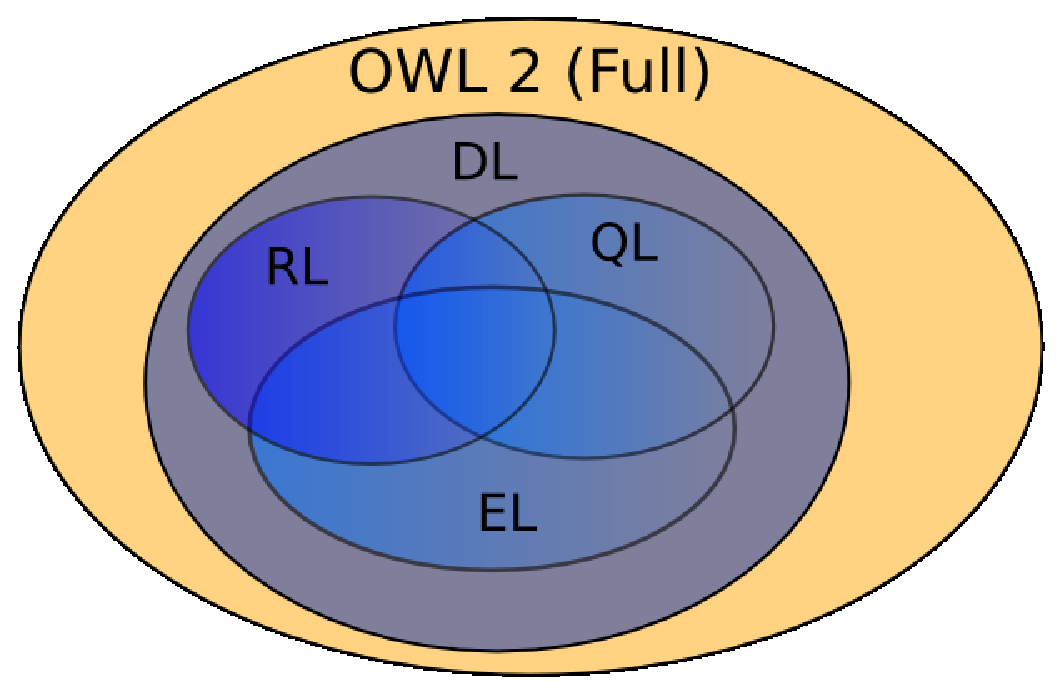
\includegraphics[width=0.6\columnwidth]{figures/owl2Profiles}
\par\end{centering}
\caption{OWL2 Profiles.\label{fig:OWL2-Profiles}}

Figura original do W3C \url{https://www.w3.org/People/Sandro/owl2-profiles-doc}
\end{figure}
 
\selectlanguage{english}%
\begin{description}
\item [{Full}] \foreignlanguage{brazil}{O perfil }OWL Full\foreignlanguage{brazil}{
é direcionado para usuários que querem a máxima expressividade e a
liberdade sintática do }OWL\foreignlanguage{brazil}{ sem garantia
computacional. É improvável que qualquer motor de raciocínio seja
capaz de suportar completamente cada recurso da }OWL Full\foreignlanguage{brazil}{
\citep{mcguinness2004owl}.}
\selectlanguage{brazil}%
\item [{DL}] O perfil \foreignlanguage{english}{OWL DL} (\foreignlanguage{english}{Description
Logic}) é para aplicações que necessitam de máxima expressividade,
enquanto mantém a computabilidade (todas as conclusões são garantidas
de ser computáveis) e decidibilidade (todas as computações terminarão
em tempo finito) \citep{mcguinness2004owl}. \foreignlanguage{english}{OWL
DL} inclui as construções da linguagem \foreignlanguage{english}{OWL},
mas elas podem ser usadas somente sob certas restrições. 
\item [{EL}] O perfil \foreignlanguage{english}{OWL} 2 EL é baseado na
família EL++ de lógica descritiva (\foreignlanguage{english}{Description}
\foreignlanguage{english}{Logic}). Esse perfil é particularmente útil
em aplicações utilizando ontologias que contêm um grande número de
propriedades e/ou classes. Além disso, o \foreignlanguage{english}{OWL}
2 EL utiliza um padrão comum, utilizado em ontologias, para conceitos
e planejamento, ou seja, a combinação de conjunção e qualidades existenciais.
\selectlanguage{english}%
\item [{QL}] \foreignlanguage{brazil}{O perfil }OWL 2 QL\foreignlanguage{brazil}{
é baseado na família }DL-Lite\foreignlanguage{brazil}{ de lógica descritiva.
Esse perfil foi criado para permitir o raciocínio (}reasoning\foreignlanguage{brazil}{)
eficiente com grandes quantidades de dados estruturados de acordo
com esquemas relativamente simples. Ele fornece a maioria dos recursos
necessários para capturar modelos conceituais, tais como diagramas
de classe UML, diagramas de entidade/relacionamento, e esquemas de
banco de dados. }
\selectlanguage{brazil}%
\item [{RL}] O perfil \foreignlanguage{english}{OWL 2 RL} é voltado para
aplicações que exigem raciocínio escalável em troca de alguma restrição
de poder expressivo. Ele define um subconjunto sintático de \foreignlanguage{english}{OWL
2} que favorece a implementação utilizando tecnologias baseadas em
regras. Esse perfil pode ser utilizado na maioria das construções
\foreignlanguage{english}{OWL 2}. Porém, para permitir implementações
baseadas em regras de raciocínio, a forma como essas construções podem
ser usadas em axiomas foi restringida. 
\end{description}
\selectlanguage{brazil}%

\subsection*{Protégé}

O editor de ontologias Protégé \citep{musen2015protege}, é a ferramenta
recomendada pela comunidade para criar ontologias em formato \foreignlanguage{english}{OWL},
fornecendo:
\selectlanguage{english}%
\begin{itemize}
\item GUI Framework:\foreignlanguage{brazil}{ para suportar múltiplas vistas
da ontologia e layouts configuráveis de componentes.}
\item API:\foreignlanguage{brazil}{ para suportar o desenvolvimento de sistemas
baseados em conhecimento.}
\item Modularization\foreignlanguage{brazil}{: permite suportar a edição
de múltiplas ontologias em um mesmo entorno.}
\item Navigation\foreignlanguage{brazil}{: fornece buscas globais e locais
e hipervínculos nos editores.}
\item Refactoring tools\foreignlanguage{brazil}{: verificação de coerência
das ontologias.}
\item Reasoning:\foreignlanguage{brazil}{ compatibilidade com vários }reasoner\foreignlanguage{brazil}{
para suportar a inferência.}
\item Plug-ins\foreignlanguage{brazil}{: arquitetura extensível que suporta
diferentes tipos de }plug-ins.
\end{itemize}
\selectlanguage{brazil}%

\selectlanguage{english}%

\subsection*{Triplestores \label{subsec:Triplestore}}

\selectlanguage{brazil}%
Uma \foreignlanguage{english}{triplestore} é um tipo de banco de dados,
baseado em grafos, para armazenar e recuperar fatos (assertions).
Esses fatos são representados na forma de triplas no padrão \foreignlanguage{english}{RDF}
(Seção \ref{triplas}). Dados são armazenados em forma de redes de
objetos com vínculos rotulados entre eles \citep{rusher2003triple}.
Esse tipo bancos de dados é recomendável quando os dados tem uma estrutura
flexível, cujas relações não tem um padrão definido.

A \foreignlanguage{english}{triplestore} \foreignlanguage{english}{Blazegraph}
\footnote{\url{https://www.blazegraph.com/}} é um dos mais completos
bancos de dados baseados em grafos e com suporte SPARQL. Ela integra
as características de uma \foreignlanguage{english}{triplestore},
fornece suporte nativo à \foreignlanguage{english}{SPARQL} e implementa
o \foreignlanguage{english}{SPARQL Protocol Endpoint}. Esse último,
padroniza a comunicação com os clientes e a compatibilidade com os
sistemas web, por meio de \foreignlanguage{english}{um Endpoint} (um
endereço onde requisições em SPARQL podem ser feitas). 

O Blazegraph foi escolhido por ter código aberto (Licença GPL) e ser
compatível com os padrões da Web Semântica. Mas qualquer \foreignlanguage{english}{triplestore}
que seja compatível com os mesmos padrões (SPARQL 1.1 e RDF) pode
ser usada. As principais características dela são:
\begin{itemize}
\item Banco de dado baseado em grafo de alta performance
\item Suporte Blueprints API e RDF/SPARQL
\item Clusters de replicação altamente disponíveis (HAJournalServer) 
\item Armazenamento de dados de uma única máquina até \textasciitilde{}50B
triples/quads (RWStore) 
\item O armazenamento de dados em cluster é essencialmente ilimitado (BigdataFederation) 
\item REST API Com deployment embutida e / ou webapp (NanoSparqlServer) 
\item SPARQL 1.1 nativo 
\item RDFS+ Inferência e manutenção da verdade
\item Triples, quads, ou Reificação feita corretamente (RDR) support 
\item Gerenciador de memória Java aproveita o JVM nativo heap (no GC) 
\item API centrada em vértices(RDF\_GAS\_API) 
\item Licença dupla: GPLv2 ou commercial 
\item Assinaturas de suporte ao desenvolvedor e produção
\end{itemize}
Para desenvolver os sistemas de software, presentes neste trabalho,
foram usadas tecnologias da web semântica. Primeiramente foram desenhadas
as ontologias em formato \foreignlanguage{english}{OWL,} na ferramenta
Protégé, depois elas foram exportadas em RDF e, finalmente, integradas
no framework Decisioner, que foi implementado usando a triplestore
\foreignlanguage{english}{Blazegraph} .

\selectlanguage{english}%
O Blazegraph\foreignlanguage{brazil}{ permitiu instanciar as ontologias,
em formato }RDF,\foreignlanguage{brazil}{ suportar inferência e permitir
consultas através da linguagem }SPARQL.\foreignlanguage{brazil}{ Essas
funcionalidades foram complementadas com ferramentas para edição da
ontologia via web (Capítulo \ref{chap:Decisioner}). }

\selectlanguage{brazil}%
Além das ontologias, foi necessário fornecer um meio de definição
de conhecimento mais próximo à linguagem dos especialistas do domínio,
para suportar a definição de SADs por parte deles. A solução identificada
foi criar uma \foreignlanguage{english}{DSL} definida a seguir.
\selectlanguage{english}%

\section{Domain Specific Language (DSL)\foreignlanguage{brazil}{ }}

\selectlanguage{brazil}%
Em desenvolvimento de software e engenharia de domínio, uma linguagem
de domínio específico, em inglês \foreignlanguage{english}{\emph{Domain-Specific
Language}}\emph{ (DSL)}, é um tipo de linguagem de programação, ou
linguagem de especificação, dedicada a um domínio particular de problema
que usa expressões próprias dos especialistas daquele domínio. Um
usuário, relacionado com um domínio específico, pode usar uma DSL
sem ter experiência em desenvolvimento de software, pois a DSL está
relacionada com seu domínio de trabalho. \citet{fowler2010domain}
afirma que programadores instruem o computador no que ele deve fazer,
pois já entendem a maneira dele trabalhar, mas, com \foreignlanguage{english}{DSLs,}
é feito o inverso: o computador começa a entender o que o usuário
do domínio escreve.

Segundo \citet{Mernik:2005:DDL:1118890.1118892}, as vantagens das
DSL, em comparação com as linguagens de propósito geral, são a expressividade,
facilidade de uso e a integração com o domínio da aplicação. O conceito
não é novo, linguagens de programação de propósito especifico existem
desde o começo das linguagens de programação, mas o termo tornou-se
padrão devido à ascensão da modelagem de domínio específico. DSLs
são classificadas da seguinte forma:
\selectlanguage{english}%
\begin{itemize}
\item Domain-Specific Markup Languages\foreignlanguage{brazil}{: são linguagens
de um domínio particular com a particularidade de anotar os dados
com etiquetas para que eles sejam sintaticamente distinguíveis. Um
exemplo delas é a }Hypertext Markup Language (HTML),\foreignlanguage{brazil}{
que permite anotar dados no domínio das páginas web.}
\item Domain-Specific Modeling Languages (specification languages):\foreignlanguage{brazil}{
são linguagens que permitem especificar sistemas com o propósito de
modelá-los. São compostas de uma estrutura consistente e de um conjunto
de regras que permitem interpretar o significado dos componentes modelados.
Uma linguagem desse tipo é a }Unified Modeling Language\foreignlanguage{brazil}{
(}UML\nomenclature{UML}{Unified Modeling Language }\foreignlanguage{brazil}{),
que permite especificar sistemas de software.}
\item Domain-Specific Programming Languages:\foreignlanguage{brazil}{ são
linguagens que permitem a programação em alto nível aplicada a um
domínio especifico de conhecimento. Uma linguagem desse tipo é a linguagem
R que permite a programação de conceitos estatísticos e geração de
gráficos.}
\end{itemize}
\selectlanguage{brazil}%
Segundo o tipo de implementação, as DSLs podem ser dividas em \foreignlanguage{english}{external
DSL e internal DSL}\citep{fowler2010domain}:
\selectlanguage{english}%
\begin{description}
\item [{External\ DSL:}] \foreignlanguage{brazil}{é uma linguagem de domínio
especifico que é definida com uma sintaxe independente de outras linguagens
de programação, tendo como principal vantagem a flexibilidade. A desvantagem
é que requer um desenvolvimento de um }full\foreignlanguage{brazil}{
parser para processá-la.}
\item [{Internal\ DSL:}] \foreignlanguage{brazil}{é uma linguagem de domínio
especifico escrita dentro de uma linguagem }host\foreignlanguage{brazil}{
existente. A vantagem desse enfoque de definição de DSL é que o tempo
e custo de desenvolvimento é menor, em relação a uma DSL externa.
Linguagens desse tipo são escritas sobre uma linguagem de propósito
geral e, por isso, apresentam a desvantagem de depender das instruções
e características da linguagem }host,\foreignlanguage{brazil}{ o que,
em alguns casos, afeta a flexibilidade e expressividade da DSL que
se quer definir.}
\end{description}
\selectlanguage{brazil}%

\subsection*{Linguagem \foreignlanguage{english}{Groovy}}

\selectlanguage{english}%
Groovy\foreignlanguage{brazil}{ é uma linguagem dinâmica para a máquina
virtual Java (}JVM\foreignlanguage{brazil}{) \citep{koenig2007groovy}.
Ela tem uma sintaxe parecida com Java, suporte para programação funcional,
produz }JVM bytecodes\foreignlanguage{brazil}{ e interopera bem com
código e bibliotecas Java. Traz características de linguagens como
}Python\foreignlanguage{brazil}{, }Ruby\foreignlanguage{brazil}{ e
}Smalltalk\foreignlanguage{brazil}{ para uma linguagem similar a Java
\citep{koenig2007groovy}.}

\selectlanguage{brazil}%
O grande benefício que \foreignlanguage{english}{Groovy} traz para
este projeto é o suporte que a sua natureza dinâmica dá ao desenvolvimento
de DSLs. Essas DSLs podem rodar diretamente na \foreignlanguage{english}{JVM}
e usar bibliotecas Java já existentes. DSLs em \foreignlanguage{english}{Groovy}
se integram facilmente à própria linguagem Groovy, de modo que não
é aparente onde o código em \foreignlanguage{english}{Groovy} termina
e a DSL começa \citep{dearle2015groovy}. Isso permite que a DSL seja
implementada como uma DSL interna, estendendo a linguagem Groovy (e
simplificando a sua criação), mas mantenha uma sintaxe próxima à linguagem
usada pelos especialistas de domínio. Como uma DSL interna, ela pode
usar ferramentas já existentes para auxiliar a escrita de código em
Groovy, como editores com \foreignlanguage{english}{\textit{syntax
highlighting}} e \foreignlanguage{english}{\textit{code completion}},
para a sua edição.

Outra vantagem de Groovy é que ela é uma linguagem para a \foreignlanguage{english}{JVM}
e existem muitas bibliotecas, em Java, que dão suporte às tecnologias
da Web Semântica. Isso inclui bibliotecas como a \foreignlanguage{english}{OWL
API}, para trabalhar com ontologias em \foreignlanguage{english}{OWL},
Apache \foreignlanguage{english}{Jena}, para acesso a \foreignlanguage{english}{triplestores},
entre outras. Finalmente, os SADs a serem criados serão aplicativos
web, Groovy tem um web framework completo e amadurecido, o Grails\foreignlanguage{english}{
}\footnote{\selectlanguage{english}%
\url{https://grails.org/}\selectlanguage{brazil}%
}. 

Grails usa uma abordagem de convenção sobre configuração que usa opções
default razoáveis. Ele se integra bem com a JVM e tem características
como ORM integrado, DSLs, metaprogramação durante runtime e compile-time,
e programação assíncrona \citep{smith2009grails}.

Uma DSL pode suportar a definição do comportamento de um SAD, fornecendo
uma solução compatível com os termos usados pelos especialistas. Isso
facilita que eles possam especificar o comportamento de um SAD com
um alto grau de detalhamento, suficiente para diminuir ou evitar a
necessidade de intervenção de desenvolvedores de software. Especialistas
podem se tornar, na prática, programadores de seus próprios SADs.

Neste projeto, DSLs servem para customizar o comportamento dos SADs.
Por isso, uma \foreignlanguage{english}{Domain-Specifc Programming
Language }em Groovy foi desenvolvida. Ela faz uso da ontologia para
organizar o conhecimento do domínio e definir o comportamento dos
SADs. 

\section{Considerações finais}

A partir do problema identificado e da revisão da literatura, foi
concluído que o desenvolvimento de ontologias é um área de pesquisa
(abrangida pela Web Semântica) que permite desenvolver sistemas web
baseados em conhecimento, satisfazendo os requisitos de desenvolvimento
do SAD SustenAgro (Capítulo \ref{chap:SAD}).

Porém, a definição de uma ontologia não é uma tarefa trivial, existem
dificuldade, por parte dos especialistas do domínio, para formalizar
ontologias. Diante deste cenário, foram analisadas varias soluções
e encontrou-se que, fornecendo ferramentas simplificadas para edição
e complementando ontologias com uma DSL, é possível facilitar a definição
dos conceitos de um SAD e seu comportamento por especialistas.

No próximo capítulo, será apresentado o Framework Decisioner. Ele
faz uso das tecnologias, abordadas neste capítulo, para definir um
framework que facilita a definição de conhecimento dos especialistas
com a finalidade de gerar SADs.


\chapter{Framework Decisioner\label{chap:Decisioner}}

Neste capítulo é apresentado o sistema Decisioner, principal contribuição
do projeto desenvolvido, ele gerá Sistemas de Apoio à Decisão e está
composto por ontologias para representar o conhecimento e por uma
DSL que permite gerenciar os conceitos e estabelecer as configurações
gerais por parte de especialistas do domínio para gerar o SAD.

Os SADs segundo a descrição feita no capitulo \ref{chap:Context}
estão compostos por banco de dados, base de modelos, base de conhecimento
e a GUI como componentes principais, os quais foram organizados em
componentes baseados na Web Semântica e nas DSL com a finalidade de
desenhar um sistema gerador de SAD. 

\section{Arquitetura do Decisioner}

A arquitetura de um software define a organização em termos de seus
componentes, suas interconexões, suas interações e também suas principais
propriedades \citet{de1997software}. Ela fornece as informações de
como os elementos envolvidos nela se relacionam. Arquiteturas trabalham
a parte externa das ligações entre seus elementos, implementações
internas desses elementos não são considerados arquiteturais \citet{sei2006architecture}.

Para encontrar e configurar componentes de software de uma arquitetura,
uma opção é descrever esses componentes, usando uma ontologia, e usar
os termos dessa ontologia para encontrar os componentes corretos para
uma aplicação \citet{Linhalis2010}. Essas ontologias podem ser criadas
utilizando linguagens padrões da Web Semântica, como a Web Ontology
Language (OWL), para melhor portabilidade \citet{Pahl2007}. Ontologias
e padrões da Web Semântica serão abordados com mais profundidade no
próximo capítulo.

Devido ao fato de que os elementos básicos de todo o SAD (Figura \ref{fig:Componentes-SAD})
serem muito parecidos, é possível criar uma arquitetura que possa
ser re\nobreakdash-usada em diferentes SADs (ou classes de SADs).
Esta arquitetura pode ser baseada em componentes de software re\nobreakdash-usáveis.
Programadores podem usar essa arquitetura e re\nobreakdash-usar os
componentes de software, já desenvolvidos para ela, para implementar
SADs mais rapidamente.

Como especialistas de domínio não têm um conhecimento muito detalhado
sobre linguagens de especificação de sistemas, é necessário o desenvolvimento
de uma \foreignlanguage{english}{Domain Specific Languag}e (DSL) adequada
ao nível de conhecimento de computação dos especialistas. Essa linguagem
também deve conter termos familiares ao domínio desses especialistas. 

Após uma pesquisa bibliográfica não foi possível encontrar sistemas
que propusessem a geração automática de interface para Sistemas de
Apoio a Decisão (SADs) com ou sem o uso de ontologias. Os artigos
encontrados mais próximos ao tema deste trabalho tratam do uso de
ontologias ou de frameworks em SADs para a área de sustentabilidade,
área que vai ser usada neste trabalho para teste dos sistemas desenvolvidos. 

O modelo geral desta solução é apresentado na Figura \ref{fig:Interfaces},
na qual as ontologias representam o banco de dados, base de modelos
e base de conhecimento, permitindo a integração e padronização desses
componentes, ditas ontologias são gerenciadas pela DSL que permite
definir o comportamento do SAD e finalmente é integrado o sistema
de GUIs que permite visualizar o SAD por meio de uma interface Web,
suportando assim o componente visual dos SAD.

O processo de definição dos SAD são controlados pela DSL, disponibilizando
aos especialistas do domínio uma linguagem especializada e de fácil
uso para definir e configurar os SAD segundo o critério deles, o conjunto
destes três componentes foi intitulado Decisioner.

\begin{figure}[H]
\centering{}\includegraphics[width=0.8\columnwidth]{\string"figures/Decisioner Architecture\string".png}\caption{Arquitetura do Decisioner\label{fig:Interfaces}}
\end{figure}

\begin{enumerate}
\item Ontologia de interfaces gráficas: ontologia que representa as interfaces
gráficas de usuários e os tipos de dados, fazendo um mapeamento entre
os dois.
\item TripleStore: sistema de armazenamento e recuperação da informação
que padroniza as informações em formato de triplas, permitindo a compatibilidade
e o reúso das informações entre fontes de dados externas.
\item Sistema gerador de interfaces gráficas: Sistema que usa a ontologia
de interfaces gráficas e as definições feitas na DSL para gerar as
interfaces gráficas Web, que compõem os SADs gerados pelo Decisioner.
\end{enumerate}

\section{Trabalhos relacionados}

Sobre as ontologias na interface gráfica encontramos: no artigo de
\citet{ruiz2006using} é analisado o uso de ontologias na engenharia
de software, identificando 50 tipos de uso entre as quais foram identificados
dois usos no suporte de interfaces gráficas.

\citet{paulheim2012ontology} propõem a seguinte definição, uma \foreignlanguage{english}{ontology-enhanced
user} interface é uma interface cujas capacidades de visualização,
possibilidades de interação, ou processo de desenvolvimento estão
habilitados ou (pelo menos) melhorado pelo emprego de uma ou mais
ontologias, na pesquisa foram identificados três propósitos para os
quais são usadas as ontologias no melhoramento das interfaces gráficas,
e são os seguintes:
\begin{enumerate}
\item Melhorar as capacidades de visualização;
\item Melhorar as possibilidades de interação;
\item Melhorar o processo de desenvolvimento;
\end{enumerate}
são apresentados os usos mais comuns de ontologias que suportem interfaces
gráficas (ontology-enhanced user interface), eles

\section{Metodologia}

Com a finalidade de desenvolver o modelo de geração de SAD anteriormente
dito, foi escolhido um caso de uso que corresponde a um SAD para avaliação
da sustentabilidade intitulado SustenAgro, o qual foi requerido pelos
especialistas em sustentabilidade da Embrapa Meio Ambiente.

O desenvolvimento dos componentes do Decisioner foram realizados da
seguinte maneira:
\begin{enumerate}
\item Seleção da \foreignlanguage{english}{Triplestore}: foi realizado um
processo de avaliação das \foreignlanguage{english}{triplestores}
existentes com a finalidade de definir uma que adapta-se nos requisitos
do sistema Decisioner.
\item Seleção da linguagem de programação e framework web: foi realizado
uma verificação das tecnologias de desenvolvimento de sistema web
compatíveis com as tecnologias da web semântica e com as DSLs.
\item Design da DSL:
\item Desenvolvimento do interprete DSL:
\item Integração com tencologias de Web Components:
\item Desenvolvimento de modulo de geração de GUIs.
\item Desenvolvimento do DSL editor:
\item Desenvolvimento do Ontology Editor:
\end{enumerate}
Os componentes da arquitetura do SustenAgro não são exclusivos do
SustenAgro, podendo ser reusados em outros SADs, os quais foram generalizados
para suportar a geração de outros tipos de sistema.

\subsection{Ontologia Decisioner}

Sobre as ontologias sobre interfaces gráficas, no artigo de \citet{ruiz2006using}
é analisado o uso de ontologias na engenharia de software, identificando
50 tipos de uso entre os quais foram identificados dois usos no suporte
de interfaces gráficas.

\citet{paulheim2012ontology} propõem a seguinte definição, uma \emph{ontology-enhanced
user interface} é uma interface cujas capacidades de visualização,
possibilidades de interação, ou processo de desenvolvimento estão
habilitados ou, pelo menos, melhorados pelo emprego de uma ou mais
ontologias. Na pesquisa foram identificados três propósitos para os
quais são usadas as ontologias no melhoramento das interfaces gráficas:
\begin{enumerate}
\item Melhorar as capacidades de visualização;
\item Melhorar as possibilidades de interação;
\item Melhorar o processo de desenvolvimento;
\end{enumerate}
Foram apresentados também os usos mais comuns de ontologias que suportam
interfaces gráficas (ontology-enhanced user interface).

Além disso, na literatura, existem pesquisas relacionadas com o vocabulário
\emph{AGROVOC Agricultural Vocabulary} \footnote{http://aims.fao.org/agrovoc}
que é um \foreignlanguage{english}{\emph{thesaurus}} que fornece termos
padronizados sobre alimentação, nutrição, agricultura, pesca, floresta
e meio ambiente criados de maneira colaborativa e coordenados pela\emph{
}\foreignlanguage{english}{Food and Agriculture Organization} (FAO\nomenclature{FAO}{Food and Agriculture Organization}).
Esses termos podem ser reutilizados nas ontologias \citep{DCMIPro841},
permitindo uma padronização dos identificadores dos conceitos, reutilizando
informações e integrando os conceitos com outros dados. Essa reutilização
foi feita através da vinculação da AGROVOC ao sistema \emph{AOS/CS
Agricultural Ontology Service Concept Server}, a FAO desenvolveu um
modelo base para esse novo sistema utilizando o \emph{OWL Web Ontology
Language.}

Cada uma destas pesquisas fornece um exemplo do uso das tecnologias
da web semântica na criação de soluções baseadas em conhecimento.
Isso é confirmado por \citet{roussey2010ontologies} por meio da descrição
de (i) como as ontologias têm sido usadas para múltiplas tarefas,
uma das quais é conseguir interoperabilidade entre sistemas de informação
heterogêneos; e de (ii) como as seguintes gerações de sistemas de
informação utilizariam uma base do conhecimento do domínio. Dadas
as afirmações dessas pesquisas, pode-se deduzir que uma ontologia
pode proporcionar o suporte conceitual para cumprir os requisitos
de sistema SAD, como o SustenAgro.

A ontologia de Sistema Apoio à Decisão contem os elementos que foram
abstraidos a partir do analise dos sistemas SAD usados pela Embrapa
Meio Ambiente em seus processos de avaliação.

Os sistemas software de avaliação que foram analisados foram:
\begin{enumerate}
\item Sistema SustenAgro: avaliação da sustentabilidade agricola em cana-de-açúcar.
\item Sistema Innova-Tec: avaliação do impacto da inovação tecnológica.
\item Sistema Nano-Tec: avaliação do impacto das nanotecnologias.
\end{enumerate}
A partir desses sistemas foram identificados elementos comuns, que
foram abstraidos na ontologia SAD com o proposito de generalizar as
classes da ontologia sustenagro, para fornecer a geração de interfaces
gráficas .

As classes idenficadas e modeladas são:
\begin{itemize}
\item Evaluation Object: classe que representa os objetos que serão analisados
em cada processo de avaliação, os quais vão ficar como indivíduos
desta classe ou de alguma subclasse dela, no caso do sistema SustenAgro
a classe \textit{Production Unit }é subclasse do Evaluation Object.
\item Feature: classe que representa as caraterísticas de um Evaluation
Object que serão quantificadas, analisadas e usadas no processo de
geração de resultados do processo de avaliação, pelo geral as Features
tem uma propriedade numérica que a quantifica.
\item Analysis: classe que vincula o resultado de uma avaliação, o nome
e data da avaliação, assim como o Evaluation Object, para representar
uma avalição
\item Value: classe que representa os valores que são atribuídos a cada
instancia de Feature.
\item User: classe que representa os usuários do sistema.
\item Role: classe que representa os tipos de usuário do sistema, relacionando
as permissões de cada tipo, por padrao tem estão instanciados os perfis
User e Admin
\end{itemize}
Na figura \ref{fig:Modelagem-do-SAD} é apresentada a modelagem basica
da estrutura de um SAD, com as classes que foram obtidas a partir
da abstração da ontologia SustenAgro.

\begin{figure}[H]
\centering{}\includegraphics[scale=0.5]{\string"figures/DSS ontology\string".png}\caption{Modelagem abstracto do SAD\label{fig:Modelagem-do-SAD}}
\end{figure}

A classe \textit{Value }representa os valores que são relacionados
com cada característica da unidade produtiva, o qual esta subdividido
nas classes \textit{Categorical }ou \textit{Real, }no caso de SustenAgro
representa os possíveis valores que um \textit{Indicator} ou \textit{Variable}
pode ter, os elementos discretos e definidos como os categóricos são
modelados como indivíduos da classe, permitindo assim, restringir
as opções de escolha.

Na figura \ref{fig:Modelagem-de-Value} é apresentado a classe \textit{Value}
e as subclasses modeladas, tanto \textit{Categorical} para conjunto
finito de valores e \textit{Real} para valores numéricos, como exemplo
está a classe \textit{Yes/No} que representa os valores de sim e não,
os quais são modelados como indivíduos de dita classe.

Cada individuo da classe \textit{Value} tem a propriedade \textit{as
number }que relaciona um valor numérico para definir um critério de
comparação e fornecer um formato para este tipo de dados.

\begin{figure}[H]
\begin{centering}
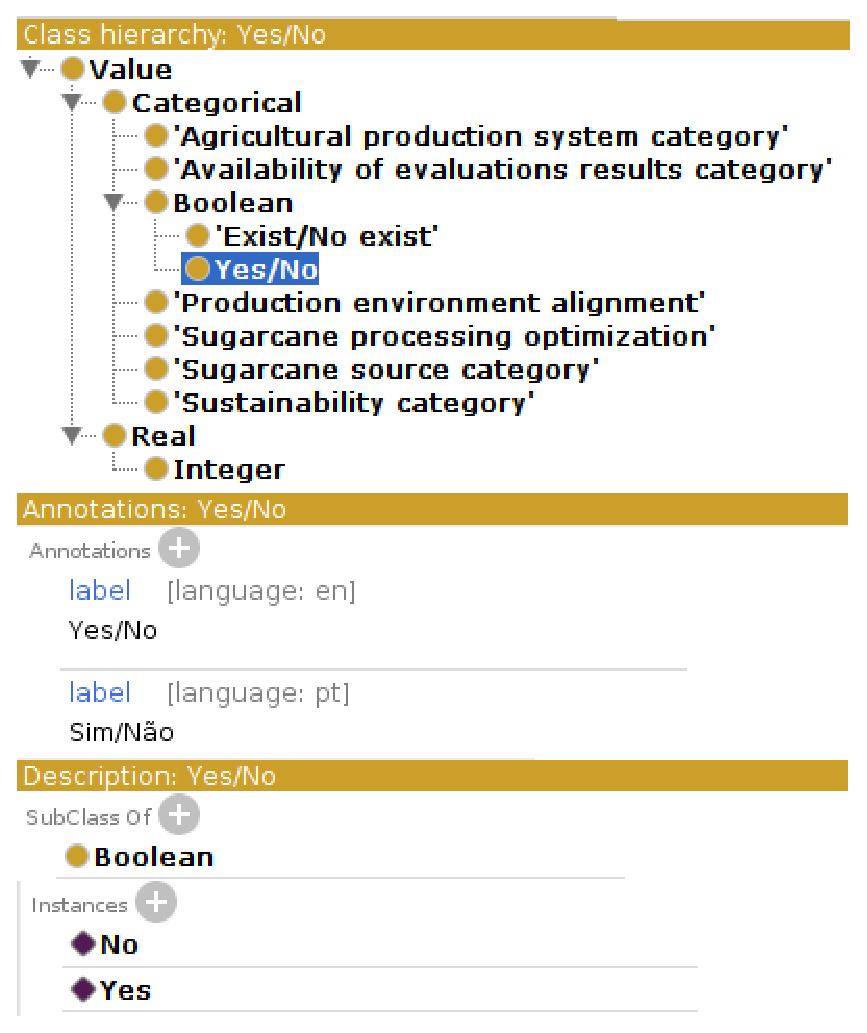
\includegraphics[scale=0.5]{figures/Value}
\par\end{centering}
\caption{Modelagem de Value\label{fig:Modelagem-de-Value}}
\end{figure}

Estas classes são complementadas com propiedades como rdfs:range ou
por padrões dos dados que relacionam as widgets mais apropriadas na
representação de informações, e assim fornecer a geração de interfaces
graficas de usuário.

A partir do anterior formato a classe 

Para definir a ontologia de domínio do SustenAgro, realizou-se uma
pesquisa das fontes de dados relacionadas com ontologias do domínio
de avaliação de sustentabilidade em sistemas produtivos de cana-de-açúcar.
Concluiu-se que não existem ontologias que suportem esse domínio,
por isso propõe-se desenvolver uma ontologia que utilize os conceitos
de avaliação de sustentabilidade e de sistemas agrícolas. Ela deve
fazer uso da pesquisa realizada por \citet{oliveira:2013} e de algumas
tecnologias fornecidas pela FAO. Essa ontologia terá a finalidade
de fornecer uma base conceitual e tecnológica para suportar o processo
de avaliação de sustentabilidade no sistema produtivo da cana\nobreakdash-de\nobreakdash-açúcar
no estado de São Paulo.

O desenvolvimento dessa ontologia ocorrerá de forma ágil e modular,
por meio de técnicas de prototipação rápida, que serão de âmbito e
complexidade crescente, abrangendo grupos de conceitos relacionados
entre si.

O desenvolvimento da ontologia depende essencialmente da comunicação
entre os especialistas e os modeladores. Foram definidos meios de
comunicação e de representação do conhecimento: reuniões presenciais
e virtuais, e o modelos conceituais que permitem uma visualização
direta do domínio.

Inicialmente, o modelo conceitual vai ser representado por meio de
um mapa conceitual que permitirá a comunicação em um formato reconhecido
por cada um dos profissionais envolvidos no projeto. Esse modelo será
representado em OWL (pelos modeladores) e serão definidas instâncias
para cada uma das classes. Depois disso, o especialista do domínio
construirá perguntas de interesse, com as quais os modeladores definirão
consultas que o sistema deverá responder segundo os resultados esperados,
conseguindo validar e ajustar até ter um protótipo confiável.

O conhecimento do domínio envolvido no sistema Sustenagro está em
contínua construção. Por isso, é necessário um enfoque que permita
realizar mudanças na estrutura e no conteúdo usados no sistema durante
seu desenvolvimento. As ontologias permitem representar o conhecimento
de um domínio por meio de formatos, como a linguagem OWL, permitindo
separar o conhecimento das outras partes do sistema.

A ontologia do domínio foi desenvolvida baseada nas definições feitas
pelos especialistas, que foram generalizadas a través das seguintes
classes representadas na Figura \ref{fig:StructureOfDomainOntology},
cada uma delas permite representar os conceitos gerais dos sistemas
de avaliação da sustentabilidade.

Também permite a integração de conceitos, inclusive quando pertencem
a domínios sem relação aparente. Um exemplo disso é a inter-relação
do conhecimento de sustentabilidade com conhecimento de interfaces
gráficas de usuário, que suporta a geração de SAD para avaliação da
sustentabilidade, o conhecimento modelado foi dividido em duas ontologias,
avaliação de sustentabilidade e do SAD.

As ontologias da web semantica são compatíveis com as tecnologias
web, permitindo o uso e integração por outros sistemas dado que está
em um formato padronizado.

\begin{figure}
\begin{centering}
\includegraphics[scale=1.5]{figures/StructureOfDomainOntology}
\par\end{centering}
\caption{Estrutura Geral da Ontologia de Domínio\label{fig:StructureOfDomainOntology}}
\end{figure}

A classe \foreignlanguage{english}{\textit{Analysis}} representa o
conceito de avaliação de sustentabilidade onde cada individuo dela
representa uma avaliação cadastrada no sistema. 

A classe \foreignlanguage{english}{\textit{EvaluationObject}}\textit{
}representa os objetos que serão avaliados pelo SAD, os quais tem
indicadores que permitem suportar o processo de avaliação.

A classe \foreignlanguage{english}{\textit{Feature}} representa cada
uma das características dos objetos de avaliação, principalmente indicadores
que são usados durante o processo de avaliação

A classe \foreignlanguage{english}{\textit{Indicator}} representa
o conceito de indicador que representa cada conceito a avaliar

A classe \foreignlanguage{english}{\textit{Weighted}} representa o
conceito de indicador vinculado com um peso que permite atribuir uma 

Ontologia de controles de gráficos: a finalidade dessa ontologia é
dar suporte a composição de controles gráficos relacionados com os
indicadores. Esse é um requisito funcional do software, uma vez que
os indicadores podem ter diversos tipos de unidades e para cada tipo
existe um tipo de controle gráfico mais apropriado para sua representação.
Por exemplo, para representar um indicador de sustentabilidade do
tipo numérico é recomendável usar um controle visual tipo spinner.

O sistema gerador de interfaces gráficas permite suportar aspectos
de usabilidade e flexibilidade ao sistema. Essa última característica
constitui uma nova proposta de desenvolvimento de SADs que permite
a adaptação automática (ou semi\nobreakdash-automática) da interface
às mudanças dos conceitos do domínio.

Será desenvolvida uma ontologia para interfaces gráficas focada na
definição e modificação de controles de usuário. Um exemplo do uso
dessa ontologia é nos indicadores. Eles armazenam um valor inserido
pelo usuário, que pode ser de diversos tipos como numérico continuo,
numérico discreto, percentagem, booleano, lista de termos ou alfanumérico.
Dada essa diversidade, é importante representar os diversos tipos
de controles gráficos em uma linguagem do domínio do especialista,
para que possam ser usados para \foreignlanguage{english}{input} da
definição dos indicadores e que faça um mapeamento entre os indicadores
e os tipos de indicador que vai ser armazenado no sistema.

Esta ontologia vai suportar a DSL fornecendo uma definição formal
dos controles gráficos que serão mapeados para cada tipo de indicador,
a DSL será apresentada a continuação.

As ontologias desenvolvidas foram modelados os conceitos envolvidos
no processo de avaliação da sustentabilidade em agricultura, definindo,
classificando e relacionando cada um dos conceitos para assim permitir
o uso em outros sistemas e conseguir fazer inferência de novo conhecimento.

\section{Decisioner DSL}

No desenvolvimento da presente pesquisa foi necessário definir uma
DSL que permitisse representar as principais características do SAD
que precisávamos desenvolver, dito SAD foi desenhado para avaliar
a sustentabilidade em agricultura, pelo qual foram integrados conceitos
do domínio de conhecimento na definição dos componentes do SAD, fornecendo
uma linguagem para especialistas onde é suportada a de definição dos
SAD, as características da DSL são:

A DSL foi baseada na linguagem Groovy \citet{koenig2007groovy}, sendo
uma extensão da linguagem Groovy, devido a que esta linguagem suporta
o desenvolvimento de DSLs. Isso inclui suporte a DSL Descriptors,
arquivos Groovy que descrevem extensões \emph{domain-specific} para
o motor de inferência e assistente de conteúdo do plugin Groovy\nobreakdash-Eclipse. 

Uma outra vantagem de Groovy é a disponibilidade do Grails Framework
para a criação de aplicações Web \citet{judd2008beginning}. 

O uso da DSL por especialistas em sustentabilidade deve diminuir o
esforço necessário para se desenvolver um SAD nesse domínio.

Espera-se que, usando a DSL, os próprios especialistas vão ser capazes
de fazer parte do desenvolvimento e validação.

A DSL e o interprete conformam uma ferramenta intitulada Decisioner,
que por meio de umas declarações permite a geração de \nomenclature{SAD}{Sistema de apoio à decisão},
dita ferramenta foi a principal contribuição desta pesquisa.

\subsection{Evaluation Object}

Os SAD focados na avaliação, é necessário definir um objeto de avaliação
que permita representar as entidades a avaliar, este objeto pelo geral
tem propriedades que vão representar cada uns dos indivíduos a avaliar,
pelo qual foi definido o comando \textit{evaluationObject, }que define
a estrutura do objeto de avalização e vincula os controles visuais,
o comando tem como argumentos a URI da classe dos elementos que vão
ser avaliados e cada uma das propriedades relacionadas. No código
\ref{lis:DSL-para-defini=0000E7=0000E3o} apresenta-se uma parte da
DSL que define a classe do objeto de avaliação \textit{ProductionUnit}
e as propriedades por meio dos comandos \foreignlanguage{english}{\textit{instance}}\textit{
}e\textit{ }\foreignlanguage{english}{\textit{type}}\textit{.}

\inputencoding{latin9}\begin{lstlisting}[caption={Defini��o de Evaluation Object  },label={lis:DSL-para-defini=0000E7=0000E3o}]
evaluationObject ":ProductionUnit", {     
 instance "ui:hasName', label: ["en": "Name", "pt": "Nome"]
 instance ":hasAgriculturalProductionSystem"
 type label: ["en": "Type", "pt": "Tipo"]
}
\end{lstlisting}
\inputencoding{utf8}
O comando \foreignlanguage{english}{instance} vincula uma propriedade
definida na ontologia através da URI a qual pode estar complementada
por parâmetros que customizam a representação visual da propriedade.

O comando type vincula as subclasses da classe principal, para ser
atribuida nas intancias de Evaluation Object, no caso do Sistema SustenAgro,
dito comando identifica que as instancias de\textit{ ProductonUnit}
também podem ser um \textit{Provider} ou uma \textit{Plant}. Os parâmetros
que podem complementar os anteriores comandos são:
\begin{enumerate}
\item \textit{label}: define um texto associado
\item \textit{placeholder:} define um texto de ajuda
\item \textit{required}: define uma propriedade obrigatória
\item \textit{widget}: define um controle gráfico de usuário
\end{enumerate}

\subsection{Feature: }

O comando \textit{Feature} define as características que serão apresentadas
durante a avaliação para serem instanciadas como parte da Analysis,
ele tem como argumento uma URI que permite vincular as subclasses
da classe referenciada, as instancias destas classes serão quantificadas
mediante o processo da avaliação no qual é realizado o preenchimento
da propriedade \textit{has value }que vincula cada Feature com um
Value para quantificá-lo. No sistema SustenAgro foram estabelecidas
as Features por meio das URIs das classes: EnvironmentalIndicator,
EconomicIndicator, SocialIndicator, ProductionEfficiencyFeature e
TechnologicalEfficiencyFeature. Além disso é possível acrescentar
a inserção de \foreignlanguage{english}{\textit{features}} novas na
interface gráfica de usuário a través do parâmetro \foreignlanguage{english}{\textit{extraFeatures}}.\inputencoding{latin9}
\begin{lstlisting}[caption={Defini��o de Features}]
feature ':EnvironmentalIndicator', 'extraFeatures': true
\end{lstlisting}
\inputencoding{utf8}

\subsection{Logica de avaliação: }

O comando \textit{Report} define o tratamento quantitativo que vai
ser efetuado às \foreignlanguage{english}{\textit{Features}}, com
a finalidade de obter valores gerais ou padrões como resultado do
processo de avaliação, suportando a definição de operações logicas
e aritméticas existentes tanto das linguagens Java e Groovy, fornecendo
assim uma linguagem para edição do metodo de avaliação, permitindo
atualizar o metodo dinámicamente e em tempo de execução, ditos valores
gerais são apresentados diretamente ou por meio de \foreignlanguage{english}{\textit{widgets}}
que facilitem a representação e compreensão da avaliação do sistema.
No código seguinte apresenta-se a implementação da formula do Sistema
SustenAgro, criando variáveis resultado de operações aritméticas para
gerar resultados gerais, no caso do SustenAgro o código gera a variável
\foreignlanguage{english}{\textit{sustainability}} que representa
o índice de sustentabilidade, más pode ser definido qualquer método
computável.\inputencoding{latin9}
\begin{lstlisting}[caption={Defini��o da logica de avalia��o.}]
report {     
 environment = weightedSum(data.':EnvironmentalIndicator')
 economic = weightedSum(data.':EconomicIndicator')
 social = weightedSum(data.':SocialIndicator')
 sustainability = (environment + social + economic)/3
}
\end{lstlisting}
\inputencoding{utf8}
O comando \foreignlanguage{english}{\textit{report}} também define
as \foreignlanguage{english}{\textit{widgets}} que conformam a parte
visual do \foreignlanguage{english}{\textit{report}}, o qual pode
usar as variáveis de resultado da logica de avaliação como entrada
das \foreignlanguage{english}{\textit{widgets}} para melhorar a representação
e facilitar a compreensão dos resultados. No código seguinte apresenta-se
um exemplo de uso desta funcionalidade no sistema SustenAgro, no qual
são definidos comandos que geram as interfaces gráficas, como \textit{sustainabilityMatrix}
que usa as variáveis geradas anteriormente como argumentos.\inputencoding{latin9}
\begin{lstlisting}[caption={Defini��o dos controles visuais do report}]
report {
 evaluationObjectInfo()
 sustainabilityMatrix x: sustainability, y: efficiency
 text 'en': 'Microregion map', 'pt': 'Mapa da microregi�o'
 map data.'Microregion'
}
\end{lstlisting}
\inputencoding{utf8} Por meio dessas configurações da DSL definiu-se as interfaces gráficas
de usuário do sistema para suportar o processo de avaliação, gerando
a representação visual dos Evaluation Objects, das Features, da logica
da avaliação e da interface gráfica do report.

Esta DSL permitirá que a interface gráfica seja definida em uma linguagem
de alto nível. Ela está baseada nas duas ontologias base e permite
definir e administrar os seguintes elementos conceituais:
\begin{itemize}
\item Indicadores
\item Componentes dos indicadores
\item Limiares
\item Métodos
\item Avaliações
\item Índices
\end{itemize}
Os elementos que compõem a DSL tem controles gráficos predefinidos
e será possível parametrizar as características destes controles gráficos
visuais. Por exemplo para as propriedades de tipo numérico contínuo
tem uma \foreignlanguage{english}{\textit{widget}} que representa
os valores reais que posem ser atribuídos em aquela propriedade, dita
\foreignlanguage{english}{\textit{widget}} pode ser mudada a outra
de acordo com as preferencias dos usuários. No caso das mudanças no
design são feitas através da edição do CSS3.

\section{TripleStore}

O sistema SustenAgro será baseado nas tecnologias da web semântica,
entre as tecnologias existentes encontra-se a Triplestore que é um
banco de dados para o armazenamento e recuperação de triplas \citet{rusher2003triple}.
Para o presente projeto foi selecionada a Triplestore Parliament \footnote{http://parliament.semwebcentral.org/}
porque fornece as características: suporte nativo a SPARQL\nomenclature{SPARQL}{SPARQL Protocol and RDF Query Language}
e SPARQL/Update e implementa o SPARQL Protocol Endpoint. Esse último,
padroniza o armazenamento e recuperação da informação; e a compatibilidade
com os sistemas web por meio do Endpoint.

\section{Sistemas de apóio à decisão}

Os sistemas de apóio à decisão (SAD) ajudam no entendimento de processos
complexos, auxiliam na comparação dos fenômenos envolvidos e suportam
a análise e escolha de alternativas no processo de decisão \citep{heinzle2010semantica}.

A equipe de TI do SustenAgro determinou que o tipo de sistema mais
conveniente para o desenvolvimento seria um Sistema de Apóio à Decisão
(SAD). Com a finalidade de definir a arquitetura e a interface gráfica
desse sistema realizaram-se duas perguntas de pesquisa que orientaram
esse projeto:
\begin{itemize}
\item Como integrar o conhecimento dos especialistas em um sistema de apoio
na tomada de decisões permitindo a continua mudança do modelo do domínio?
\item Como gerar interfaces gráficas a partir de definições simples do domínio
do conhecimento?
\end{itemize}
Tendo em conta os requisitos do software, como o suporte a contínua
mudança do modelo de dados e a geração dinâmica de interfaces, se
propõe a arquitetura a seguir.

\section{Considerações finais}

Não foram encontrados trabalhos na área de geração automática de interfaces
para SADs. Nem mesmo em áreas específicas de aplicação. Também foi
encontrado pouco material sobre ontologias para descrição de interfaces
gráficas. 

Este capítulo apresentou os conceitos principais de SADs, incluindo
a definição geral e a arquitetura de software. Ele também apontou
para a necessidade da geração automática (ou semi\nobreakdash-automática)
de interfaces gráficas de usuários SADs. Uma abordagem para conseguir
a geração automática (ou semi\nobreakdash-automática) de GUIs consiste
na integração com DSLs, onde sejam definidas as características gerais
do sistema e integrado com os conceitos do domínio de conhecimento
a través das ontologias usadas nesses sistemas.

Através dos conceitos definidos nelas, será possível associar tipos
aos dados e modos de apresentação dos mesmos (por exemplo, tipos de
gráficos de apresentação), a partir dessas descrições, \foreignlanguage{english}{widgets}
podem ser geradas de maneira automática e assim suportar a geração
de SADs de maneira semiautomática.


\chapter{SAD SustenAgro\label{chap:SustenAgro}}

O Framework Decisioner organiza e gerencia os componentes gerais dos
SADs de avaliação. Cada SAD tem particularidades que precisam ser
definidas e ajustadas para configurar suas funcionalidades. As ontologias
específicas do domínio e as DSL, explicadas nos capítulos anteriores
fornecem o meio de definição dessas particularidades. 

O SAD SustenAgro foi usado como a primeira instanciação do Framework
Decisioner. Ele é composto por uma ontologia de domínio, DSL e elementos
gráficos de design (ícones, imgens de fundo, etc.) que permitem instanciá-lo
no Decisioner. Sendo seu principal componente a ontologia do domínio
de avaliação da sustentabilidade da produção de cana-de-açucar na
região centro-sul do Brasil..

Nest capítulo, serão explicadas a arquitetura, a metodologia e os
componentes mais importantes do SAD SustenAgro. Serão feitas também
algumas considerações sobre o processo de definição do SAD.

\section{Arquitetura do SustenAgro}

O SAD SustenAgro serviu de base para modelar e desenvolver os componentes
que fazem parte do Decisioner. Por isso, o processo real de desenvolvimento
dele foi muito mais complicado que uma simples instanciação de um
framework. Ele envolveu diversas iterações para determinar o que deveria
ser implementado como parte do framework e como parte da aplicação.
Para simplificar o texto e facilitar o entendimento de como o framework
Decisioner é usado para instanciar um SAD, as diversas versões do
framework não serão discutidas.

A arquitetura de um SAD implementado usando o Framework Decisioner
tem os seguintes componentes:
\begin{enumerate}
\item Ontologia do domínio: ontologia que representa os conceitos do domínio.
No caso do SustenAgro, o domínio é a avaliação da sustentabilidade
do sistema produtivo de cana-de-açúcar, na região centro-sul. Essa
ontologia é a base para o SAD pois permite estabelecer os conceitos
fundamentais, que são utilizados pelo sistema. No caso do SustenAgro,
eles são: indicadores, componentes de indicadores, índices, dimensões
da sustentabilidade, recomendações e o método de avaliação.
\item DSL: programa descrevendo a configuração e comportamento do SAD. Ele
especifica as \foreignlanguage{english}{features} do domínio a serem
usadas, as fórmulas do modelo e o aspecto e estrutura do relatório
a ser gerado. No caso do SustenAgro, as \foreignlanguage{english}{features}
são os indicadores, as formulas calculam os índices de sustentabilidade
e produtividade, e o relatório usa a Matriz e o Semáforo de Sustentabilidade.
\selectlanguage{english}%
\item Web components\foreignlanguage{brazil}{: o SustenAgro usa dois }Web
Components\foreignlanguage{brazil}{ específicos (além das oferecidas
pelo Decisioner): a Matriz de Sustentabilidade e o Semáforo de Sustentabilidade.
Ambas são implementadas usando a biblioteca Polymer da Google.}
\selectlanguage{brazil}%
\item Imagens e layout: Um conjunto de imagens e arquivos de layout (css)
compõem o \foreignlanguage{english}{look-and-feel} específico do SAD,
incluindo seu logo.
\end{enumerate}

\section{Metodologia.\label{sec:Metodologia}}

O conhecimento do domínio abrangido no sistema SustenAgro está em
contínua evolução. Por isso, foi necessário usar uma metodologia que
suporte mudanças na estrutura e nos dados do sistema, durante cada
uma das fases do desenvolvimento. O desenvolvimento da ontologia de
domínio SustenAgro foi realizada de forma ágil e modular, por meio
de técnicas de prototipação rápida, abrangendo grupos de conceitos
relacionados entre si.

O desenvolvimento da ontologia depende essencialmente da comunicação
entre os especialistas de domínio e os modeladores. Dessa forma, foram
definidos meios de comunicação (reuniões presenciais e virtuais) e
de representação do conhecimento (modelos conceituais), que permitiram
explorar o domínio. 

Um dos meios, que permitiu uma melhor comunicação, foi o desenvolvimento
de um mapa conceitual, por meio da ferramenta Cmap Tools\footnote{http://cmap.ihmc.us/},
com a participação de um grupo de especialistas em modelagem de conhecimento.
Esse processo começou em uma reunião da equipe na Embrapa Informática
Agropecuária (situada situada na Universidade Estadual de Campinas,
UNICAMP). Nessa reunião, um especialista em desenvolvimento de ontologias
da Embrapa forneceu treinamento sobre a metodologia para definir ontologias,
desenvolvimento de mapas conceituais, com os principais conceitos,
e desenvolvimento de modelos em \foreignlanguage{english}{OWL,} para
tornar esse conehcimento computável.

Após realizada a modelagem, o especialista do domínio definiu perguntas
de interesse, com as quais os modeladores (o autor e um colega de
mestrado) definiram consultas que o sistema deveria responder segundo
os resultados esperados, conseguindo validar e ajustar o modelo até
ter um protótipo confiável.

Na Figura \ref{fig:Methodology} é apresentada a metodologia para
desenvolver a ontologia SustenAgro, a qual teve vários ciclos de desenvolvimento
nos quais foram integradas novas caraterísticas.

\begin{figure}[H]
\noindent \begin{centering}
\includegraphics[width=1\columnwidth]{\string"figures/Ontology Methodology\string".eps}
\par\end{centering}
\caption{Metodologia de definição da ontologia SustenAgro.\label{fig:Methodology}}
\end{figure}

Um aspecto importante das ontologias é que elas fornecem um formato
que adapta-se às mudanças do domínio e permite separar o conhecimento
dos outros componentes do sistema.

A metodologia, que direcionou o desenvolvimento do SAD SustenAgro,
foi \foreignlanguage{english}{a SCRUM} \citep{schwaber2002gile},
que permitiu integrar práticas ágeis no desenvolvimento do sistema.
Nesse contexto, o termo ágil refere-se ao desenvolvimento em tempos
curtos e geração de protótipos facilmente adaptáveis às mudanças.
Cada uma das etapas da metodologia foi realizada várias vezes e, por
isso, foi necessário redesenhar os componentes. As metodologias ágeis
são cíclicas e os protótipos mudam em cada ciclo para cumprir os novos
requisitos.

\label{A-metodologia-de-UI}A metodologia de desenvolvimento dos \foreignlanguage{english}{Web
Components} e das \foreignlanguage{english}{Web UI}  tiveram um enfoque
baseado em \foreignlanguage{english}{User Centered Design}. A avaliação
dessas duas interfaces foi realizada integradamente para validar
se os requisitos identificados. 

O processo de design das \foreignlanguage{english}{web UI} incluiu
as seguintes etapas de levantamento de requisitos:
\begin{enumerate}
\item Descrição de \foreignlanguage{english}{User Stories:} técnica de desenvolvimento
ágil que permite descrever características do software desde a perspectiva
do usuário. Ela fornece uma identificação dos usuários, das funcionalidades
e explica o porque uma dita funcionalidade é necessária. 
\item Descrição de \foreignlanguage{english}{Scenarios:} técnica de desenvolvimento
ágil que permite descrever detalhadamente as características das \foreignlanguage{english}{user
stories}.
\item Descrição de \foreignlanguage{english}{Storyboard\emph{s:}} descreve
cada uma das interações do usuário com o sistema em uma determinada
tarefa, visualizando a interação como uma história em quadrinhos.
\item Descrição de \foreignlanguage{english}{\emph{Mockups:}} design do
esboço da interface gráfica do sistema. Eles foram analisados pelos
especialistas da Embrapa, para avaliar se atendiam às funcionalidades
básicas descritas no levantamento dos requisitos.
\item Desenvolvimento de protótipo visual: A partir da validação dos \foreignlanguage{english}{Mockups,}
foi desenvolvido um protótipo da interface gráfica, com a finalidade
de que os especialistas do domínio avaliassem se as interfaces cumpriam
com os requisitos.
\end{enumerate}
Cada uma dessas etapas de desenvolvimento, foram realizadas sempre
em parceria com os especialistas do domínio. Isso foi importante para
realizar o levantamento correto de requisitos tanto das web UI como
das funcionalidades do SAD, identificadas a partir destas técnicas.
Todo esse processo foi necessário pois não existia uma definição especifica
do que os especialistas precisavam.

\section{Ontologia de domínio: SustenAgro\label{sec:Ontologia-do-dom=0000EDnio}}

A ontologia SustenAgro representa o conhecimento necessário para suportar
avaliação de sustentabilidade no sistema produtivo de cana-de-açúcar
na região centro-sul do Brasil. Ela representa conceitos por meio
de entidades, classes, relações semânticas e axiomas. Esses elementos
organizam e representam a realidade modelada. 

Para definir a ontologia SustenAgro, realizou-se uma pesquisa das
fontes de dados relacionadas com ontologias do domínio de avaliação
de sustentabilidade em sistemas produtivos de cana-de-açúcar. Concluiu-se
que não existem ontologias que suportassem esse domínio. Por isso,
propôs-se desenvolver uma ontologia que utilizasse conceitos sobre
avaliação de sustentabilidade e sistemas agrícolas. Essa ontologia
representa conceitos gerais de conceitos identificados na literatura
e conceitos particulares ao SustenAgro, identificados por \citet{oliveira:2013}. 

Deve-se destacar que a ontologia SustenAgro abrange um domínio bem
específico: sustentabilidade de sistemas produtivos de cana-de-açucar
na região centro-sul do Brasil. Acreditamos que essa é uma característica
deste tipo de SAD. Modelamentos desse tipo tendem a ser específicos.
No caso do Sustenagro, ele abrange apenas um só sistema produtivo
em uma região específica.

A figura \ref{fig:ontology-conceptual-map} representa um mapa conceitual
com os principais conceitos modelados no SustenAgro e como eles estão
relacionados entre si. As etiquetas, em cada relação dos conceitos,
permitem identificar a relação entre os dois conceitos.

As ontologias da web semântica permitem separar o conhecimento do
domínio da lógica da computação, independizando o desenvolvimento
destes aspectos do SAD.

\begin{figure}[H]
\begin{centering}
\includegraphics[width=0.8\columnwidth]{\string"figures/SustenAgro conceptual map\string".eps}
\par\end{centering}
\caption{Mapa conceitual da ontologia SustenAgro.\label{fig:ontology-conceptual-map}}
\end{figure}

Para conseguir que a ontologia SustenAgro fosse computável, foi necessário
defini-la na linguagem \foreignlanguage{english}{OW}L (fornecendo
uma representação compreensível por humanos e computadores). O editor
de ontologias Protégé\footnote{\url{http://protege.stanford.edu/}}
foi usado, permitindo modelar o conhecimento e exportar ele ao formato
\foreignlanguage{english}{RDF}, para ser compatível com sistemas \foreignlanguage{english}{triple-stores}
(seção \ref{subsec:Triplestore}) \citep{allemang2011semantic}. 

\selectlanguage{english}%
Triplestores\foreignlanguage{brazil}{ suportam a realização de consultas
complexas para permitir a resposta a perguntas de interesse aos usuários
do sistema.  Esta caraterística permite a recuperação da informação
com significado semântico, permitindo que os sistemas deem respostas
às consultas complexas de interesse. Também o RDF suporta a integração
de conhecimento externo existente em formatos da web semântica, como
são vários sistemas de representação do conhecimento como dicionários,
}thesaurus\foreignlanguage{brazil}{ e redes semânticas, o que permite
aumentar as possibilidades de desenvolvimento de novas funcionalidades. }

\selectlanguage{brazil}%
A ontologia do SustenAgro modela o conhecimento dos especialistas
baseando-se na ontologia do Decisioner (Figura \ref{fig:Modelagem-do-SAD}).
Ela inclui a ontologia Decisioner e define conceitos gerais dos SADs.
Isso é obrigatório, pois o código do framework Decisioner entende
os conceitos da ontologia SustenAgro apenas porque eles também são
conceitos válidos derivados da ontologia Decisioner. Exemplos de conceitos/classes
modelados são: \foreignlanguage{english}{\textit{Production Unit}}\textit{,
}\foreignlanguage{english}{\textit{Microregion, Indicator}}\textit{,}
\foreignlanguage{english}{\textit{Categorical}}. A partir dessas classes
foi possível desenvolver o modelo de dados em \foreignlanguage{english}{OWL}, 

As classes da ontologia SustenAgro são relacionados por meio de \foreignlanguage{english}{\textit{Object
Properties}} e \foreignlanguage{english}{\textit{Data Properties}}
que permitem vincular semanticamente as instâncias das classes. A
principal contribuição da ontologia do domínio é ser uma representação
semântica do conhecimento de domínio, tanto para os usuários como
para o sistema computacional, tornando-se um meio de comunicação entre
os especialistas de domínio e os programadores.

Nas próximas seções, serão apresentadas as principais classes modeladas
na ontologia do domínio de avaliação da sustentabilidade (SustenAgro).
\selectlanguage{english}%

\subsection*{Production Unit}

\selectlanguage{brazil}%
Representa as organizações que podem ser avaliadas pelo sistema SustenAgro.
Atualmente elas podem ser \textit{Fornecedores de cana-de-açúcar}
e / ou \textit{Usinas processadoras de cana-de-açúcar}. Cada processo
de avaliação requer dados que identifiquem as unidades produtivas
através de propriedades que as definam.

Esta classe tem propriedades obrigatórias como:
\selectlanguage{english}%
\begin{itemize}
\item hasAgriculturalProductionSystem\foreignlanguage{brazil}{: relaciona
o sistema de produção agrícola em avaliação.}
\selectlanguage{brazil}%
\item hasAvailabilityOfEvaluationResults: relaciona o tipo de disponibilização
dos resultados.
\item hasSugarcaneSource: relaciona a origem da cana.
\item harvestYear: define o ano da safra.
\item canavialLongevity: define a longevidade do canavial.
\end{itemize}
\selectlanguage{brazil}%
A Figura \ref{fig:Modelagem-unidade-produtiva} apresenta a modelagem
da classe \foreignlanguage{english}{Production Unit}, feita na ferramenta
Protégé.

\begin{figure}[H]
\noindent \begin{centering}
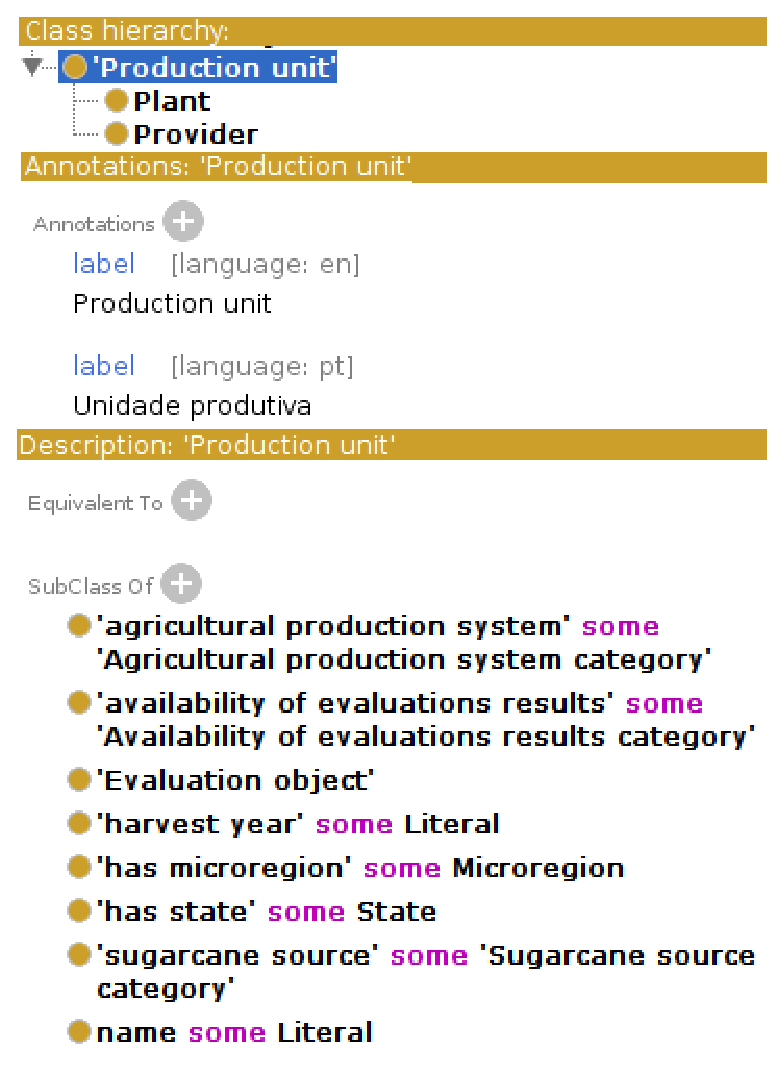
\includegraphics[width=0.6\columnwidth]{figures/ProductionUnit}
\par\end{centering}
\caption{Modelagem da classe de unidade produtiva (ProductionUnity). \label{fig:Modelagem-unidade-produtiva}}
\end{figure}

\selectlanguage{english}%

\subsection*{\textit{Microregion}\foreignlanguage{brazil}{\textit{ }}}

\selectlanguage{brazil}%
Representam os locais onde são localizadas as unidades produtivas.
É permitido definir a microrregião onde as fazendas e usinas do sistema
produtivo de cana-de-açúcar se localizam. Atualmente, a ontologia
tem os 7 estados pertencentes ao centro-sul do Brasil e as 243 microrregiões
dentro desses estados. Esses dados foram originalmente obtidos por
consulta SPARQL à \foreignlanguage{english}{DB-pedia} e integrados
à ontologia.

A Figura \ref{fig:Modelagem-de-Microrregi=0000E3o} mostra a modelagem
das localizações geográficas usadas no sistema SustenAgro, com algumas
instâncias de \foreignlanguage{english}{\textit{Microregion}}.

\begin{figure}[H]
\noindent \begin{centering}
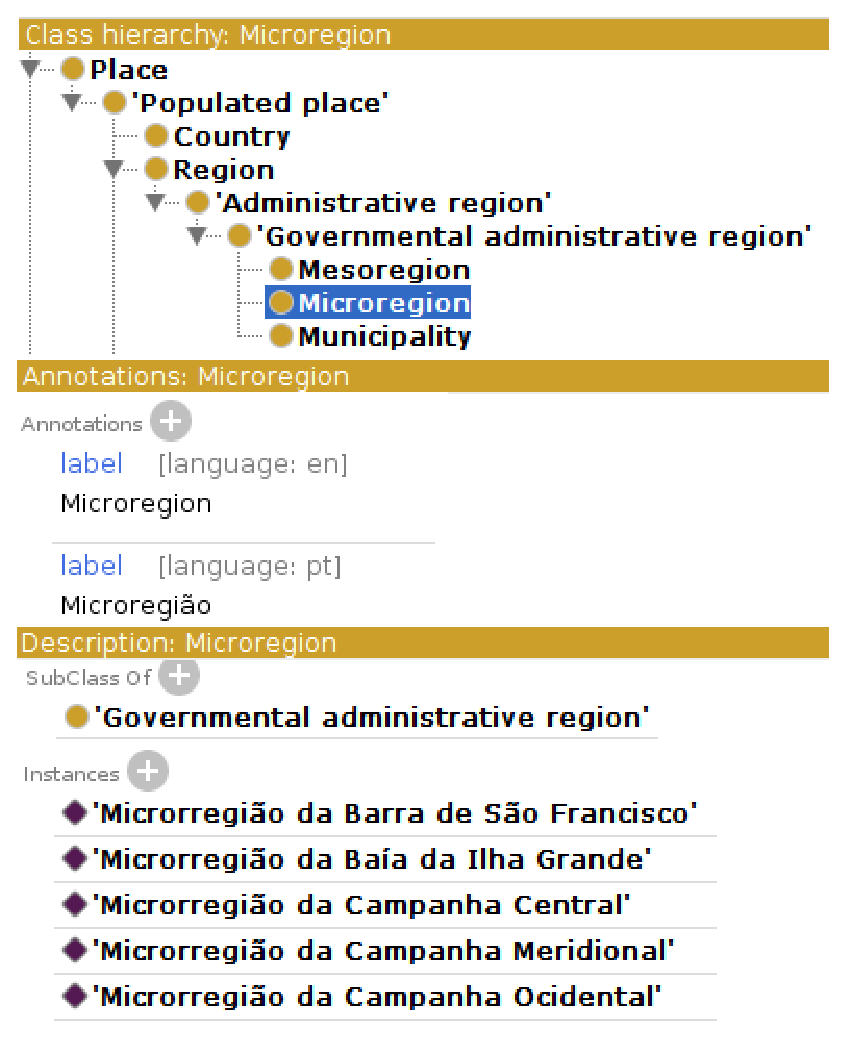
\includegraphics[width=0.6\columnwidth]{figures/Microregion}
\par\end{centering}
\caption{Modelagem de microrregiões.\label{fig:Modelagem-de-Microrregi=0000E3o}}
\end{figure}

\selectlanguage{english}%

\subsection*{\textit{Indicator}}

\selectlanguage{brazil}%
Os indicadores são o principal componente da ontologia. Eles foram
propostos por um grupo de especialistas de diversas áreas da produção
agrícola e sustentabilidade \citep{oliveira:2013}. 

Eles representam as características das unidades produtivas que serão
identificadas e quantificadas em cada processo de avaliação. Eles
tem uma propriedade \foreignlanguage{english}{\textit{Value}}\textit{
}que quantifica a sustentabilidade do indicador.

Também permite a integração de conceitos, inclusive quando pertencem
a domínios sem relação aparente. Um exemplo disso é a inter-relação
do conhecimento de sustentabilidade com conhecimento de interfaces
gráficas de usuário, que suporta a geração de SAD para avaliação da
sustentabilidade. O conhecimento foi dividido em duas ontologias,
avaliação de sustentabilidade e outra dos componentes gerais de um
SAD.

A Figura \ref{fig:Modelagem-de-Indicador} apresenta a hierarquia
dos indicadores, que está subdividida em \foreignlanguage{english}{Efficiency
Indicator} e \foreignlanguage{english}{Sustainability Indicator}.
Os \foreignlanguage{english}{Indicators} têm a propriedade \foreignlanguage{english}{\textit{has
value}}\textit{ }que vincula indivíduos da classe \foreignlanguage{english}{\emph{Value}}\textit{
}que representa as opções de resposta dos indicadores\textit{ .}
Existe outra propriedade, \foreignlanguage{english}{has weight,} que
é opcional e estabelece um peso para o indicador\foreignlanguage{english}{\textit{.}}

A Figura \ref{fig:Modelagem-de-Indicador} mostra o indicador intitulado
\foreignlanguage{english}{\textit{Adequacy of boilers}}. Na propriedade
\foreignlanguage{english}{\textit{has value}} ele tem uma restrição
que limita os valores dessa propriedade a valores de uma lista de
valores categóricos. A propriedade \foreignlanguage{english}{\textit{has
weight}} também tem uma restrição que limita seus valores a instâncias
da classe \foreignlanguage{english}{\textit{Sugarcane process Optimization}}.

\begin{figure}[H]
\noindent \begin{centering}
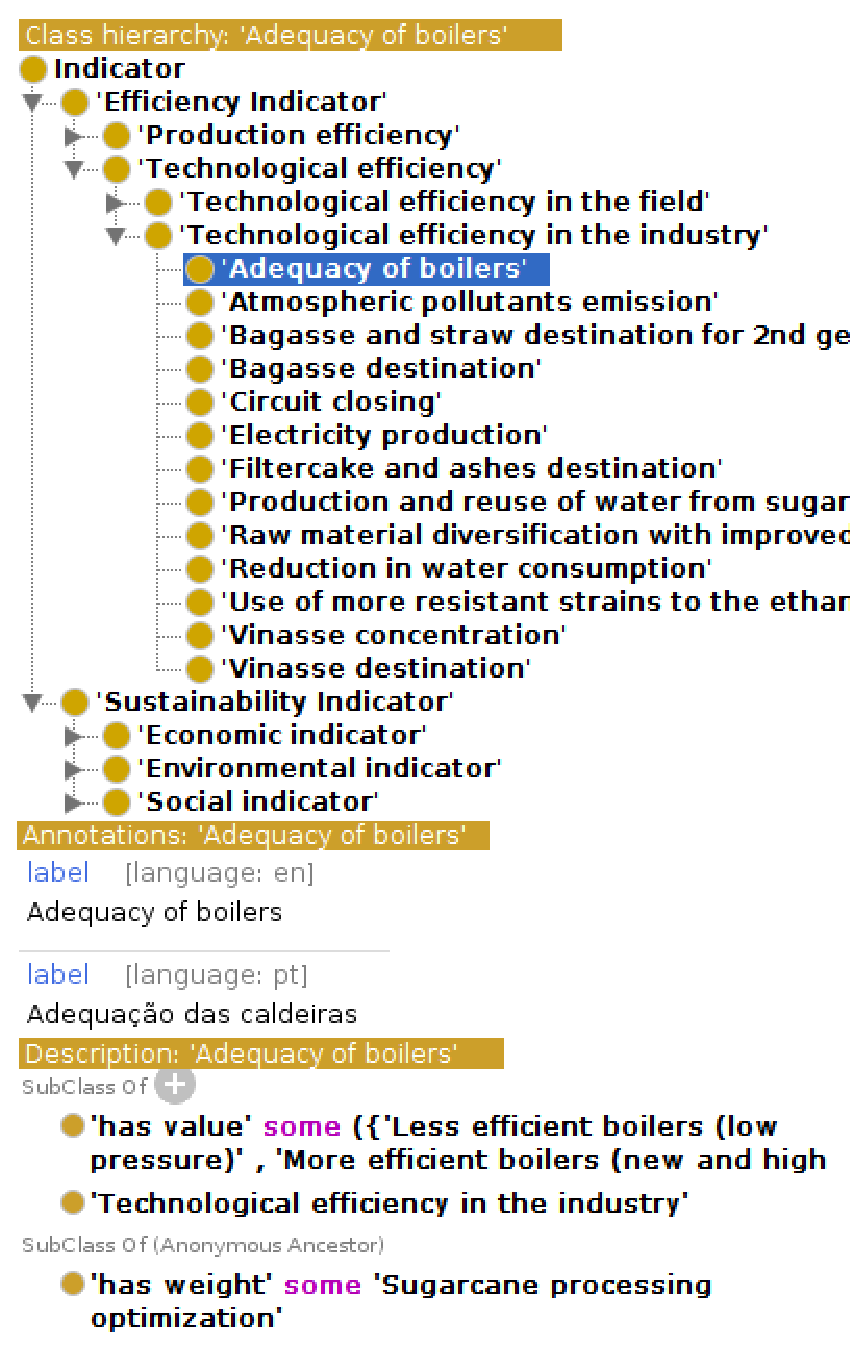
\includegraphics[width=0.6\columnwidth]{figures/Indicador}
\par\end{centering}
\caption{Modelagem de indicador \label{fig:Modelagem-de-Indicador}}
\end{figure}

Segundo a descrição do método de avaliação (Capítulo \ref{chap:Sustainability_Assessment}),
os indicadores de sustentabilidade são classificados em três dimensões
de sustentabilidade: dimensão ambiental, dimensão social e dimensão
econômica. Tendo as três uma participação equitativa no método de
avaliação \citep{kraines2011system}. 

A continuação serão apresentados cada uma das três dimensões.

\subsubsection*{Dimensão ambiental}

Nesta dimensão não foi possível identificar indicadores de tipo hídrico.
Não existe consenso entre os especialistas consultados sobre quais
são os aspectos mais relevantes deles para a avaliação da sustentabilidade,
porém, é um aspecto fundamental para trabalhar nas futuras etapas
de pesquisa. 

A dimensão de indicadores ambientais, está composta dos seguintes
conceitos:

\begin{itemize}
\item Atributo solo (\foreignlanguage{english}{Soil Attribute}): indicadores
que avaliam os aspectos referentes às características do solo.
\item Atributo hídrico (\foreignlanguage{english}{Hydric Attribute}): indicadores
que avaliam os aspectos referentes à disponibilidade e qualidade das
fontes hídricas.
\item Atributo clima (\foreignlanguage{english}{Weather Attribute}): indicadores
que avaliam os aspectos climáticos.
\end{itemize}

\subsubsection*{A dimensão social}

Nesta dimensão é importante reconhecer que as unidades produtivas,
sejam do tipo fazendas ou usinas, têm vínculos com pessoas tanto internamente
como externamente. Por isso, é importante refinar os indicadores para
incluir a população externa à unidade produtiva que é afetada pelas
práticas produtivas.

A Agência Paulista de Tecnologia dos Agronegócios (APTA\nomenclature{APTA}{Agência Paulista de Tecnologia dos Agronegócios})
forneceu dados econômicos das principais usinas do estado de São Paulo,
que permitiram definir a dimensão econômica das unidades produtivas
na ontologia de domínio.

A dimensão social está composta dos seguintes conceitos:

\begin{itemize}
\item Atributo emprego e renda (\foreignlanguage{english}{Employment and
Income Attribute}): indicadores que avaliam os aspectos referentes
à mão de obra.
\item Atributo saúde (\foreignlanguage{english}{Health Attribute}): indicadores
que avaliam os aspectos de segurança dos trabalhadores.
\item Atributo treinamento (\foreignlanguage{english}{Training Attribute}):
indicadores que avaliam os aspectos da capacitação dos trabalhadores.
\end{itemize}

\subsubsection*{A dimensão econômica}

Esta dimensão está composta dos seguintes conceitos:

\begin{itemize}
\item Atributo industrial (Industrial Atribute): indicadores que avaliam
os aspectos industriais. 
\item Atributo área recuperada (Recovered Area Atribute): indicadores que
avaliam os aspectos da área produtiva e das técnicas produtivas.
\item Atributo produtividade (Porductivity Atribute): indicadores que avaliam
os aspectos dos produtos e dos processos produtivos.
\item Atributo custo (Cost Atribute): indicadores que avaliam os aspectos
dos custos da produção. 
\end{itemize}
Cada uma das três dimensões deve ser avaliada equitativamente para
gerar um resultado coerente com a teoria da sustentabilidade agrícola\citep{tilman2002agricultural}. 

\subsubsection*{Modelagem do método de avaliação SustenAgro}

A Figura \ref{fig:Method} mostra um mapa conceitual dos conceitos
envolvidos na avaliação da sustentabilidade, na qual recebe como entrada
os indicadores selecionados pelos usuários e aplica as formulas de
avaliação para gerar os índices de sustentabilidade e eficiência.
 Desta maneira é possível quantificar a sustentabilidade.

\begin{figure}[H]
\begin{centering}
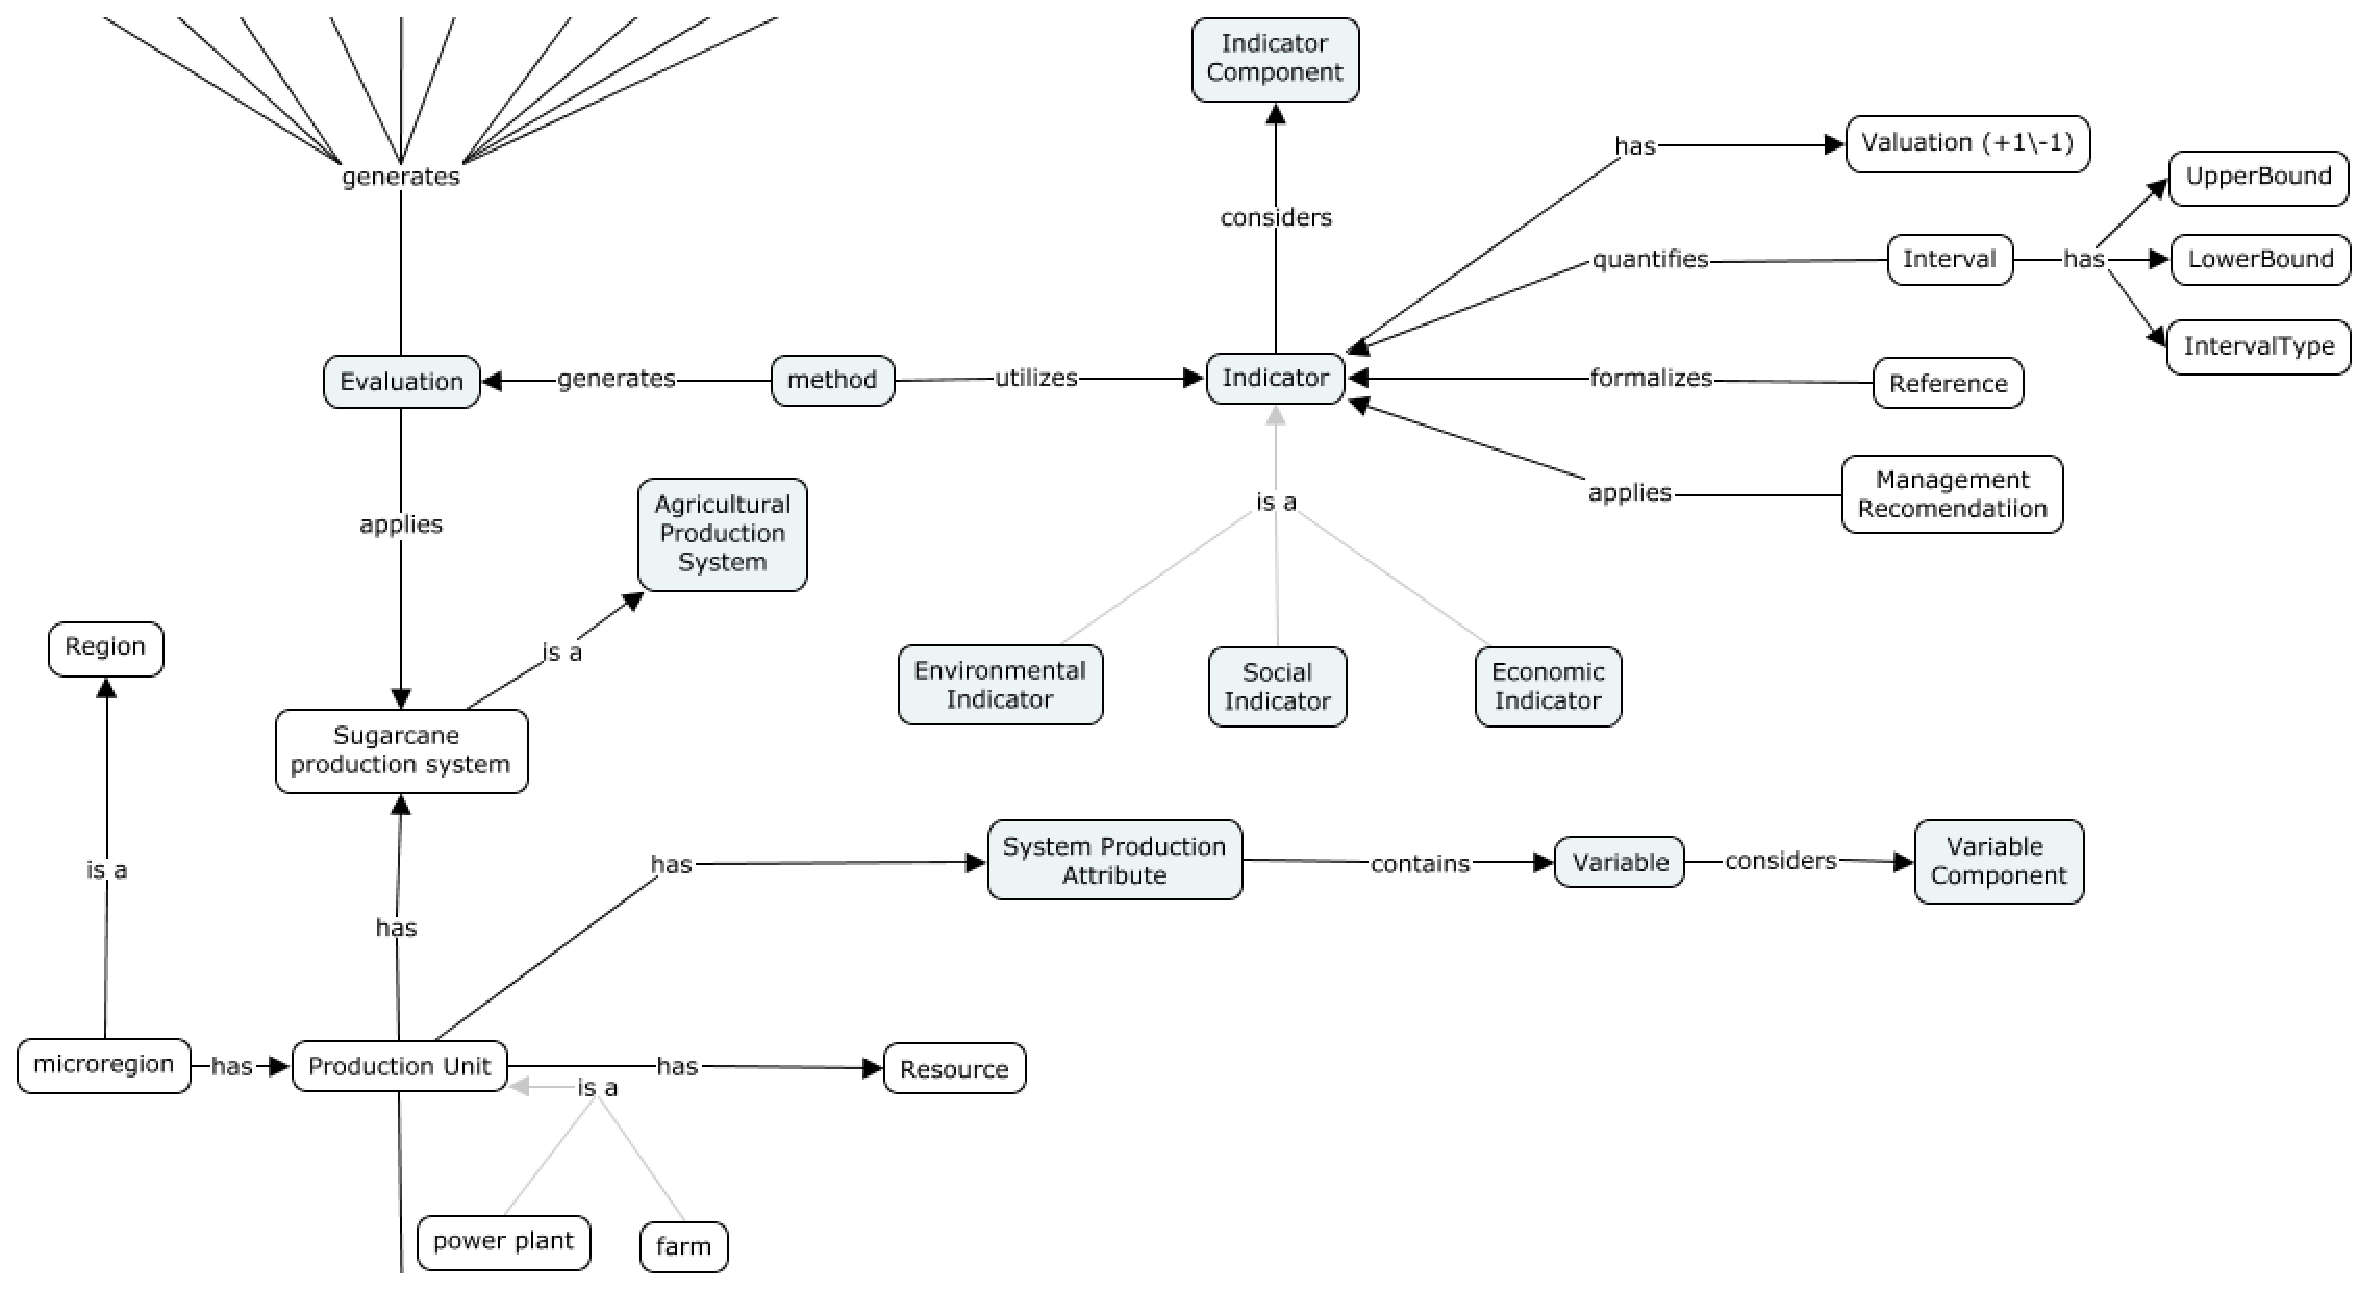
\includegraphics[width=1\textwidth]{figures/metodo}
\par\end{centering}
\caption{Mapa conceitual - Método de Avaliação.\label{fig:Method}}
\end{figure}

As dimensões da sustentabilidade permitiram organizar os indicadores,
levando essa organização desde os modelos de mapas conceituais, às
ontologias, método de avaliação e, finalmente, até a representação
dos resultados nas web UI dos SADs.
\selectlanguage{english}%

\subsection*{Subclasses of Categorical}

\selectlanguage{brazil}%
A classe \foreignlanguage{english}{Categorical} representa os possíveis
\foreignlanguage{english}{Value} discretos que um \foreignlanguage{english}{\textit{Indicator}}
pode ter na forma de categorias (por exemplo, Existe e Não Existe).
Um \foreignlanguage{english}{Value} também pode ser Real ou Inteiro.
A classe Categorical é definida na ontologia Decisioner, mas a SustenAgro
cria diversas classes filhas para definir uma série de valores categóricos.

Cada subclasse de \foreignlanguage{english}{Categorical} é composta
por um conjunto finito de elementos ou valores. Cada valor é modelado
como indivíduo da classe, permitindo assim, restringir as opções de
instanciação de cada indicador.

Na Figura \ref{fig:Modelagem-de-Value}, é apresentada a classe \foreignlanguage{english}{\textit{Value}}
e suas subclasses, tanto \foreignlanguage{english}{\textit{Categorical}}
para conjunto finito de valores e \foreignlanguage{english}{\textit{Real}}
para valores numéricos. Um exemplo de classe categórica seria a \foreignlanguage{english}{\textit{Yes/No}}
que representa os valores de sim e não e é composta pela lista de
indivíduos \foreignlanguage{english}{Yes} e No.

Cada individuo da classe \foreignlanguage{english}{\textit{Value}}
tem a propriedade \foreignlanguage{english}{\textit{as number}}\textit{
}que relaciona a ele um valor numérico. Esse valor define um critério
de comparação entre os indivíduos da mesma classe. Ele é usado nas
fórmulas do método de avaliação.

\begin{figure}[H]
\begin{centering}
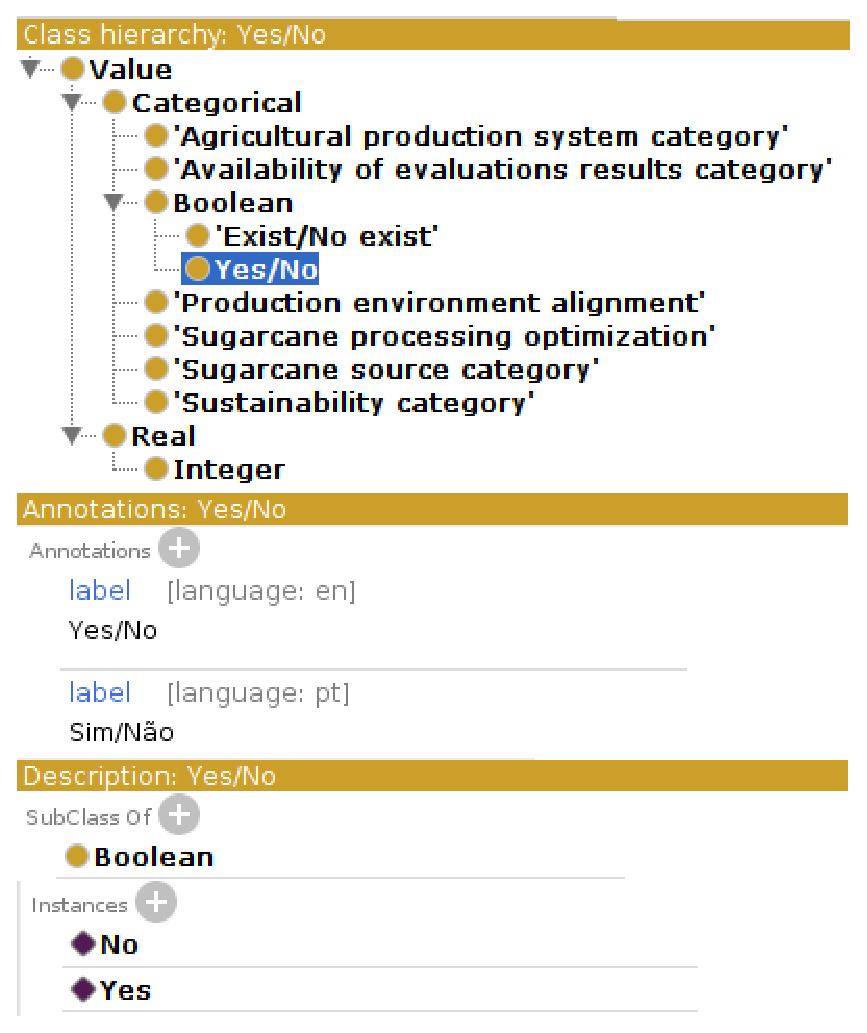
\includegraphics[scale=0.6]{figures/Value}
\par\end{centering}
\caption{Modelagem de \foreignlanguage{english}{Value}\label{fig:Modelagem-de-Value}}
\end{figure}

\selectlanguage{english}%

\section{SustenAgro Web UI\label{sec:Web-UI}}

\selectlanguage{brazil}%
O design das interfaces gráficas e desenvolvimento dos web componentes
foram realizados por meio da várias técnicas de levantamento de requerimentos
para especificar as funcionalidades que os especialistas precisavam
do sistema SustenAgro. Foram usadas as seguintes técnicas: \foreignlanguage{english}{User
Stories}, \foreignlanguage{english}{Scenarios}, \foreignlanguage{english}{Storyboard},
\foreignlanguage{english}{Mockups} e protótipo de interface gráfica.

Na fase inicial, foram definidos os perfis de usuários do SAD SustenAgro,
inicialmente definiram-se os perfis descritos a seguir: 
\begin{itemize}
\item Administrador: usuário com permissões para editar Ontologias, DSL
e web UI. Ele é o responsável pela administração do SAD e tem todas
as permissões do sistema.
\item Especialista de domínio: especialista em sustentabilidade ou afins,
com permissões para recuperar e gerenciar informações das avaliações,
gerar reportes e mudar os conceitos relacionados com os indicadores
e método de avaliação.
\item Usuário final: usuário padrão do sistema que tem permissões para realizar
avaliações de sustentabilidade em cana-de-açúcar e de gerenciar os
dados cadastrados por ele. 
\end{itemize}
No SAD SustenAgro v1.0, foi removido o perfil especialista, ficando
apenas os perfis administrador e usuário final. As funções desse perfil
foram incluídas no perfil administrador.

As técnicas realizadas para desenvolver as web UI, são descritas a
seguir.
\selectlanguage{english}%

\subsection*{User Stories}

\selectlanguage{brazil}%
Histórias de usuário são uma técnica para descrever, de uma forma
curta e simples, as características do sistema a partir da perspectiva
do usuário ou cliente do sistema, gerando uma definição de alto nível
de um requisito. O padrão é: como um “tipo de usuário”, quero atingir
“algum objetivo” para “alguma finalidade”.

Na aplicação dessa técnica foram obtidas as seguintes histórias:
\begin{enumerate}
\item O usuário poderá identificar e cadastrar a localização geográfica
e a área da sua lavoura (definir região geográfica do IBGE, latitude
e longitude - a partir do \foreignlanguage{english}{Google Maps}). 
\item O usuário poderá identificar e cadastrar a microrregião a que pertence
a sua lavoura. O sistema fará uma sugestão de cadastro a partir dos
dados da localização geográfica.
\item O usuário deverá preencher o estado de cada indicador específico nas
dimensões ambiental, econômica e social, devendo adaptar-se às condições
das regiões e microrregiões do Brasil.
\item O usuário poderá obter o resultado dos índices, segundo a informação
preenchida e a fórmula de agregação dos indicadores.
\item O usuário poderá armazenar a informação dos indicadores para futuras
consultas.
\item O usuário poderá acrescentar indicadores que considere importantes
para a análise. Deve-se estabelecer regras para essa funcionalidade
de tal modo que os novos indicadores (criados pelos usuários) sejam
recuperáveis de um modo separado dos indicadores cadastrados no sistema. 
\item O sistema deve fornecer um cronograma de avaliação, sendo recomendado
realizar a avaliação depois de cada safra.
\end{enumerate}
\selectlanguage{english}%

\subsection*{Scenarios}

\selectlanguage{brazil}%
É uma técnica que permite a descrição das funcionalidades do sistema
desde a perspectiva do usuário ou cliente, realizando uma descrição
detalhada de cada um dos passos dos usuários no sistema para completar
uma tarefa. A seguir serão apresentadas as 8 histórias de usuários
do SAD SustenAgro com os cenários associados:

\textbf{História de usuário \#1:} “O usuário poderá identificar e
cadastrar a localização geográfica e a área da sua lavoura (definir
região geográfica do IBGE, latitude e longitude - a partir do \foreignlanguage{english}{Google
Maps}).”
\begin{enumerate}
\item O usuário ingressa na conta dele, através do sistema web SustenAgro
em \url{http://sustenagro.embrapa.br}, e o sistema apresenta a tela
“\foreignlanguage{english}{Home}” 
\item O usuário seleciona a aba “unidades produtivas” e dá um \foreignlanguage{english}{click}
em ``cadastrar unidade produtiva'', o sistema apresenta a tela de
cadastro de unidades produtivas, onde tem um mapa do \foreignlanguage{english}{Google
Maps} 
\item O usuário seleciona no mapa um ponto que identificará a localização
da unidade produtiva, se ele quiser, também é possível marcar a área
da lavoura para que o sistema possa ter dados mais específicos para
o processo de avaliação de sustentabilidade. Uma vez terminado, o
usuário dá um \foreignlanguage{english}{click} no botão “próximo”
e o sistema cadastra a informação preenchida. 
\end{enumerate}
\textbf{História de usuário \#2}: “O usuário poderá identificar e
cadastrar a microrregião a que pertence a unidade produtiva dele,
por meio de uma sugestão que o sistema faz com os dados da localização
geográfica.”
\begin{enumerate}
\item O usuário poderá fazer a “Historia de usuário \#1” ou entrar no sistema
e continuar com o cadastro da unidade produtiva de onde ele tenha
parado. O sistema apresentará uma tela com sugestões de microrregiões. 
\item O usuário poderá escolher a microrregião, onde esteja localizada a
unidade produtiva, e salvá-la no sistema por meio do botão ``próximo''. 
\end{enumerate}
\textbf{História de usuário \#3:} “O usuário deverá preencher o estado
de cada indicador específico nas dimensões ambiental, econômica e
social. Esses indicadores devem adaptar-se às condições das regiões
e microrregiões do Brasil, da mesma forma as faixas de limiares de
sustentabilidade foram definidas.''
\begin{enumerate}
\item O usuário poderá fazer a “História de usuário \#2” ou entrar no sistema
e continuar com o cadastro dos indicadores de onde ele tenha parado.
O sistema apresentará uma tela com três abas que contém os controles
que permitirão fazer o cadastro dos indicadores nas dimensões ambiental,
econômica e social. 
\item O usuário dá um \foreignlanguage{english}{click} na primeira aba e
começa a preencher os dados dos indicadores ambientais, principalmente
os limiares que identificam o estado do indicador. A interface também
permite eliminar ou acrescentar indicadores específicos, por parte
dos usuários (funcionalidade que é explicada na “Hstória de usuário
\#4”). 
\item O usuário preenche os dados das outras duas dimensões e o sistema
salva as mudanças.
\end{enumerate}
\textbf{História de usuário \#4:} “Permitir o emprego da metodologia
para avaliação caso a caso: possibilitar que o usuário selecione quais
indicadores vai utilizar. Dentro dos indicadores, ele pode recomendar
limiares mais adequados para a sua realidade, também pode inserir
novos indicadores\slash{}limiares.”
\begin{enumerate}
\item O usuário poderá fazer a “Historia de usuário \#3” ou entrar no sistema
e continuar na tela de cadastro de indicadores e, quando acontecer
que o usuário precise de um indicador que não seja oferecido pelo
sistema, o usuário poderá acrescentá-lo por meio do botão “acrescentar
indicador” 
\item O usuário dá um \foreignlanguage{english}{click} no botão “acrescentar
indicador” e lhe é apresentada uma interface de entrada, onde ele
deverá cadastrar o título, a descrição, os limiares, a medida do manejo
e a justificativa desse indicador. Em seguida preencher o estado do
indicador. O sistema salva esses dados inseridos. 
\item O usuário também poderá eliminar alguns indicadores segundo seu critério.
\end{enumerate}
\textbf{História de usuário \#5:} \textquotedbl{}O usuário poderá
obter o resultado dos índices segundo a informação preenchida e a
formula de agregação dos indicadores.\textquotedbl{}
\begin{enumerate}
\item Depois de terminada a “História de usuário \#4”, o sistema fará a
avaliação, que foi definida no sistema pelos especialistas. 
\item O resultado da avaliação será cadastrado no sistema com informações
sobre a metodologia utilizada.
\item A metodologia de avaliação pode ser atualizada pelos administradores
para uso em avaliações futuras.
\end{enumerate}
\textbf{História de usuário \#6:} ``O usuário poderá armazenar a
informação dos indicadores para futuras consultas.''
\begin{enumerate}
\item O usuário preenche alguns indicadores nos formulários do SustenAgro. 
\item Esses dados serão salvos quando o usuário mudar de formulário ou quando
der um \foreignlanguage{english}{click} no botão ``próximo''.
\end{enumerate}
\textbf{História de usuário \#7:} ``O usuário poderá acrescentar
indicadores que considere importantes para sua análise, devem-se estabelecer
regras para essa funcionalidade de tal modo que os novos indicadores
(criados pelos usuários) sejam recuperáveis de um modo separado dos
indicadores cadastrados no sistema.''
\begin{enumerate}
\item Quando o usuário estiver preenchendo os indicadores gerados pelo sistema,
o sistema fornecerá um conjunto de controles que permitam a inclusão
de um novo indicador. Esse novo indicador será definido pelo próprio
usuário baseado na sua experiência na área. 
\item O sistema armazenará esse novo indicador com uma classificação especial
que permita sua identificação e separação dos outros indicadores. 
\item O usuário poderá preencher os dados do novo indicador, para que sejam
inclusos na avaliação de sustentabilidade.
\end{enumerate}
\textbf{História de usuário \#8:} ``Cronograma de avaliação, depois
de cada safra.''
\begin{enumerate}
\item Depois de fazer o cadastro da fazenda e das culturas que são plantadas
nela, o sistema poderá identificar quando termina cada safra, gerando
um alerta para que o usuário faça o processo de avaliação nessa data.
\item O usuário lerá o alerta e poderá fazer o processo de avaliação de
sustentabilidade. 
\end{enumerate}
\selectlanguage{english}%

\subsection*{Storyboard}

Storyboards\foreignlanguage{brazil}{ são similares aos cenários. Elas
ilustram a interação necessária para atingir um objetivo sem utilizar
uma lista de passos. A interação é visualizada por meio de uma história
em quadrinhos.}

\selectlanguage{brazil}%
Essa representação permite uma visão holística da interação do usuário,
com ênfase nos aspectos funcionais da interação e não nos aspectos
da interface de usuário. A seguir, são apresentados os textos das
\foreignlanguage{english}{storyboard} dos processos identificados:

A Figura \ref{fig:StoryBoard-1} apresenta o processo de cadastro
da localização da unidade produtiva, para conseguir vincular dados
a partir da localização geográfica.

\begin{figure}[H]
\begin{centering}
\includegraphics[width=1\columnwidth]{\string"figures/Stroyboard 1\string".eps}
\par\end{centering}
\centering{}\caption{\textit{\emph{\small{}StoryBoard definição da localização. \label{fig:StoryBoard-1}}}}
\end{figure}

A Figura \ref{fig:StoryBoard-2} apresenta o formulário de seleção
da microrregião que faz parte da localização descrita no \foreignlanguage{english}{storyboard}
anterior. Essa informação é importante para caracterizar a unidade
produtiva.

\begin{figure}[H]
\begin{centering}
\includegraphics[width=1\columnwidth]{\string"figures/Stroyboard 2\string".eps}
\par\end{centering}
\caption{\textit{\emph{\small{}StoryBoard seleção da unidade produtiva. \label{fig:StoryBoard-2}}}}

\end{figure}

A Figura \ref{fig:StoryBoard-3} apresenta o esquema do formulário
de preenchimento dos indicadores que permite cadastrar uma avaliação,
dito formulário é adaptável a vários tipos de dados dos indicadores,
permitindo construir interfaces amigáveis para os usuários.

\begin{figure}[H]

\includegraphics[width=1\columnwidth]{\string"figures/Stroyboard 3\string".eps}

\caption{\textit{\emph{\small{}StoryBoard mostrando o preenchimento dos indicadores.\label{fig:StoryBoard-3}}}}

\end{figure}
A Figura \ref{fig:StoryBoard-4} apresenta o processo de avaliação
para uma unidade produtiva, segundo o método Sustenagro. Ele vai processar
os indicadores preenchidos para gerar uma análise.

\begin{figure}[H]
\begin{centering}
\includegraphics[width=1\columnwidth]{\string"figures/Stroyboard 4\string".eps}
\par\end{centering}
\caption{\textit{\emph{\small{}StoryBoard}} sobre a avaliação de unidade produtiva\label{fig:StoryBoard-4}}
\end{figure}

A Figura \ref{fig:StoryBoard-5} apresenta o formulário de definição
de novos indicadores, por parte dos usuários do sistema. Eles permitem
a integração de novos conceitos ao sistema. 

\begin{figure}[H]
\begin{centering}
\includegraphics[width=1\columnwidth]{\string"figures/Stroyboard 6\string".eps}
\par\end{centering}
\centering{}\caption{\textit{\emph{\small{}StoryBoard}} para cadastro de novo indicador.\label{fig:StoryBoard-5}}
\end{figure}

A Figura \ref{fig:StoryBoard-6} apresenta o relatório resultante
do processo de avaliação. Ele é composto pelos índices, uma tabela
dos dados cadastrados , a matriz de sustentabilidade e as recomendações

\begin{figure}[H]
\begin{centering}
\includegraphics[width=1\columnwidth]{\string"figures/Stroyboard 5\string".eps}
\par\end{centering}
\caption{\textit{\emph{\small{}StoryBoard}} mostrando a apresentação de resultados\label{fig:StoryBoard-6}}
\end{figure}


\subsection*{Mockups das Interfaces do SustenAgro}

A partir das técnicas anteriores foi possível identificar as tarefas
que os usuários do sistema SustenAgro realizarão. O fluxo das tarefas
e os dados de cada um foram mudando na aplicação de cada técnica,
gerando varias definições das web UI. Uma vez identificadas as caracterizaras
essenciais da interface gráfica, procedeu-se a definir os Mockups
que permitiram criar uma representação visual das interfaces do sistema. 

O desenvolvimento dos \foreignlanguage{english}{Mockups} foram feitos
com a ferramenta \foreignlanguage{english}{Moqups} \footnote{Moqups \url{https://moqups.com/} }. 

A Figura \ref{fig:Mockup_home} mostra uma interface gráfica da tela
inicial do SAD SustenAgro . A interface mostra uma descrição do sistema,
e as principais abas, entre elas a aba de Ferramenta que permite iniciar
o processo de avaliação de sustentabilidade.

\begin{figure}[H]
\centering{}\includegraphics[width=1\columnwidth]{\string"figures/Mockup Main\string".eps}\caption{Mockup da tela inicial do SustenAgro.\label{fig:Mockup_home}}
\end{figure}

Os Mockups integram as \foreignlanguage{english}{widgets,} que permitem
avaliar a interface gráfica de uma maneira mais próxima à interface
final e assim suportar a sua avaliação por parte dos especialistas
do domínio.  

A Figura \ref{fig:Mockup_indicators} apresenta os passos do processo
de avaliação, na ordem representada pela numeração das abas. Esta
tela corresponde ao formulário de cadastro dos indicadores, que permite
cadastrar o valor correspondente a cada indicador.

\begin{figure}[H]
\centering{}\includegraphics[width=1\columnwidth]{figures/Tool_environmental_indicators}\caption{Mockup da tela de indicadores do SustenAgro.\label{fig:Mockup_indicators}}
\end{figure}

Na apresentação dos Mockups aos especialistas foram identificadas
varias mudanças para facilitar a navegabilidade da \foreignlanguage{english}{web
UI,} as mudanças corresponderam à integração de tarefas e a melhora
na apresentação dos formulários e dos resultados de avaliação. Estas
mudanças reestruturaram o \foreignlanguage{english}{look-and-feel}
do SAD. 

\subsection*{Protótipo da Interface Gráfica do SustenAgro}

A partir das melhoras dos protótipos visuais identificadas nas avaliações
dos Mockups, foram identificadas as características da web UI, com
as quais foi desenvolvido um protótipo funcional da interface gráfica
do SustenAgro, que inicialmente só permitia interagir com dados simulados.

A web UI do SAD SustenAgro, foi integrada com cada uma das funcionalidades
do SAD em cada ciclo de desenvolvimento, e actualmente está disponível
nos servidores do laboratório Intermídia do ICMC\nobreakdash-USP
\footnote{http://biomac.icmc.usp.br:8080/sustenagro/}. 

Na Figura \ref{fig:Home} é apresentada a página inicial do protótipo.

\begin{figure}[H]
\begin{centering}
\includegraphics[width=1\textwidth]{figures/home}
\par\end{centering}
\caption{Protótipo do SustenAgro – Tela incial.\label{fig:Home}}
\end{figure}

Nessa tela pode-se observar o texto explicativo da ferramenta e as
abas de ``Início'', ``Ferramenta'' e ``Contato''. A opção ``Ferramenta''
permite iniciar o processo de avaliação de sustentabilidade.

Uma vez cadastrada uma unidade produtiva, disponibiliza-se a opção
de criar nova avaliação. Essa, ação vai gerar a tela da Figura \ref{fig:Indicators},
que permite visualizar os indicadores para que os usuários preencham
cada um, segundo a realidade da unidade produtiva em avaliação. Cada
indicador tem várias opções de resposta que estão ligadas a valores
que quantificam a sustentabilidade. Esses valores estão definidos
na ontologia de sustentabilidade (a ontologia SustenAgro) e são usados
nas fórmulas para gerar os índices de sustentabilidade. 

Na Figura \ref{fig:Indicators}, é apresentado o formulário dos indicadores
de eficiência. Eles são subdivididos em eficiência de produção e tecnológica.
Na Figura \ref{fig:Indicators}, é mostrado o indicador Manejo, como
exemplo. Um tipo de manejo foi escolhido e o peso desse indicador
foi declarado como direto. Esses valores serão usados nas fórmulas
da avaliação da sustentabilidade.

\begin{figure}[H]
\noindent \begin{centering}
\includegraphics[width=1\columnwidth]{figures/SustenAgro-scenario}
\par\end{centering}
\caption{Cadastro de indicadores \label{fig:Indicators}}
\end{figure}

A partir dos dados cadastrados, são gerados os resultados do sistema.
Eles consistem na planilha de eficiência e custo, na planilha da sustentabilidade
e o relatório do sistema. As planilhas permitem visualizar os atributos
dos indicadores e a tela de relatório apresenta a matriz de sustentabilidade,
onde são relacionados os índices de eficiência e de sustentabilidade.
O relatório é apresentado na Figura \ref{fig:Planilhas-de-resultado}. 

\begin{figure}[H]
\noindent \begin{centering}
\includegraphics[width=1\columnwidth]{figures/SustenAgro-results}
\par\end{centering}
\caption{Planilhas do resultado da avaliação \label{fig:Planilhas-de-resultado}}
\end{figure}

\selectlanguage{english}%

\section{Web Components}

\selectlanguage{brazil}%
Foram desenvolvidos dois \foreignlanguage{english}{Web Components}
específicos para o SustenAgro. Eles geram gráficos específicos do
relatório solicitado pelos especialistas da Embrapa Meio Ambiente 

\subsection*{Matriz de Sustentabilidade}

Com a finalidade de suportar a geração de relatórios, no formato definido
pelos especialistas do domínio, foi necessário implementar dois \foreignlanguage{english}{Web
Component} específicos. Um deles foi a \foreignlanguage{english}{widget}
intitulada Matriz de Sustentabilidade. Ela é composta por dois eixos
que correspondem ao índice de eficiência, eixo Y, e ao índice de sustentabilidade,
eixo X. Os índices tem magnitudes que são dividas em segmentos que
permitem dividir a área em doze quadrantes da sustentabilidade. Cada
avaliação realizada com o método SustenAgro gerará dois índices que
são localizados em um quadrante da matriz de sustentabilidade. Cada
quadrante está relacionado com uma recomendação específica. 

A Figura \ref{fig:Matriz-de-sustentabilidade-widget} mostra a implementação
desse \foreignlanguage{english}{Web Component,} mostrando resultados
reais de uma avaliação, com o índice de sustentabilidade avaliado
em 2.33 e o índice de eficiência avaliado em 2.4.

\begin{figure}[H]
\noindent \begin{centering}
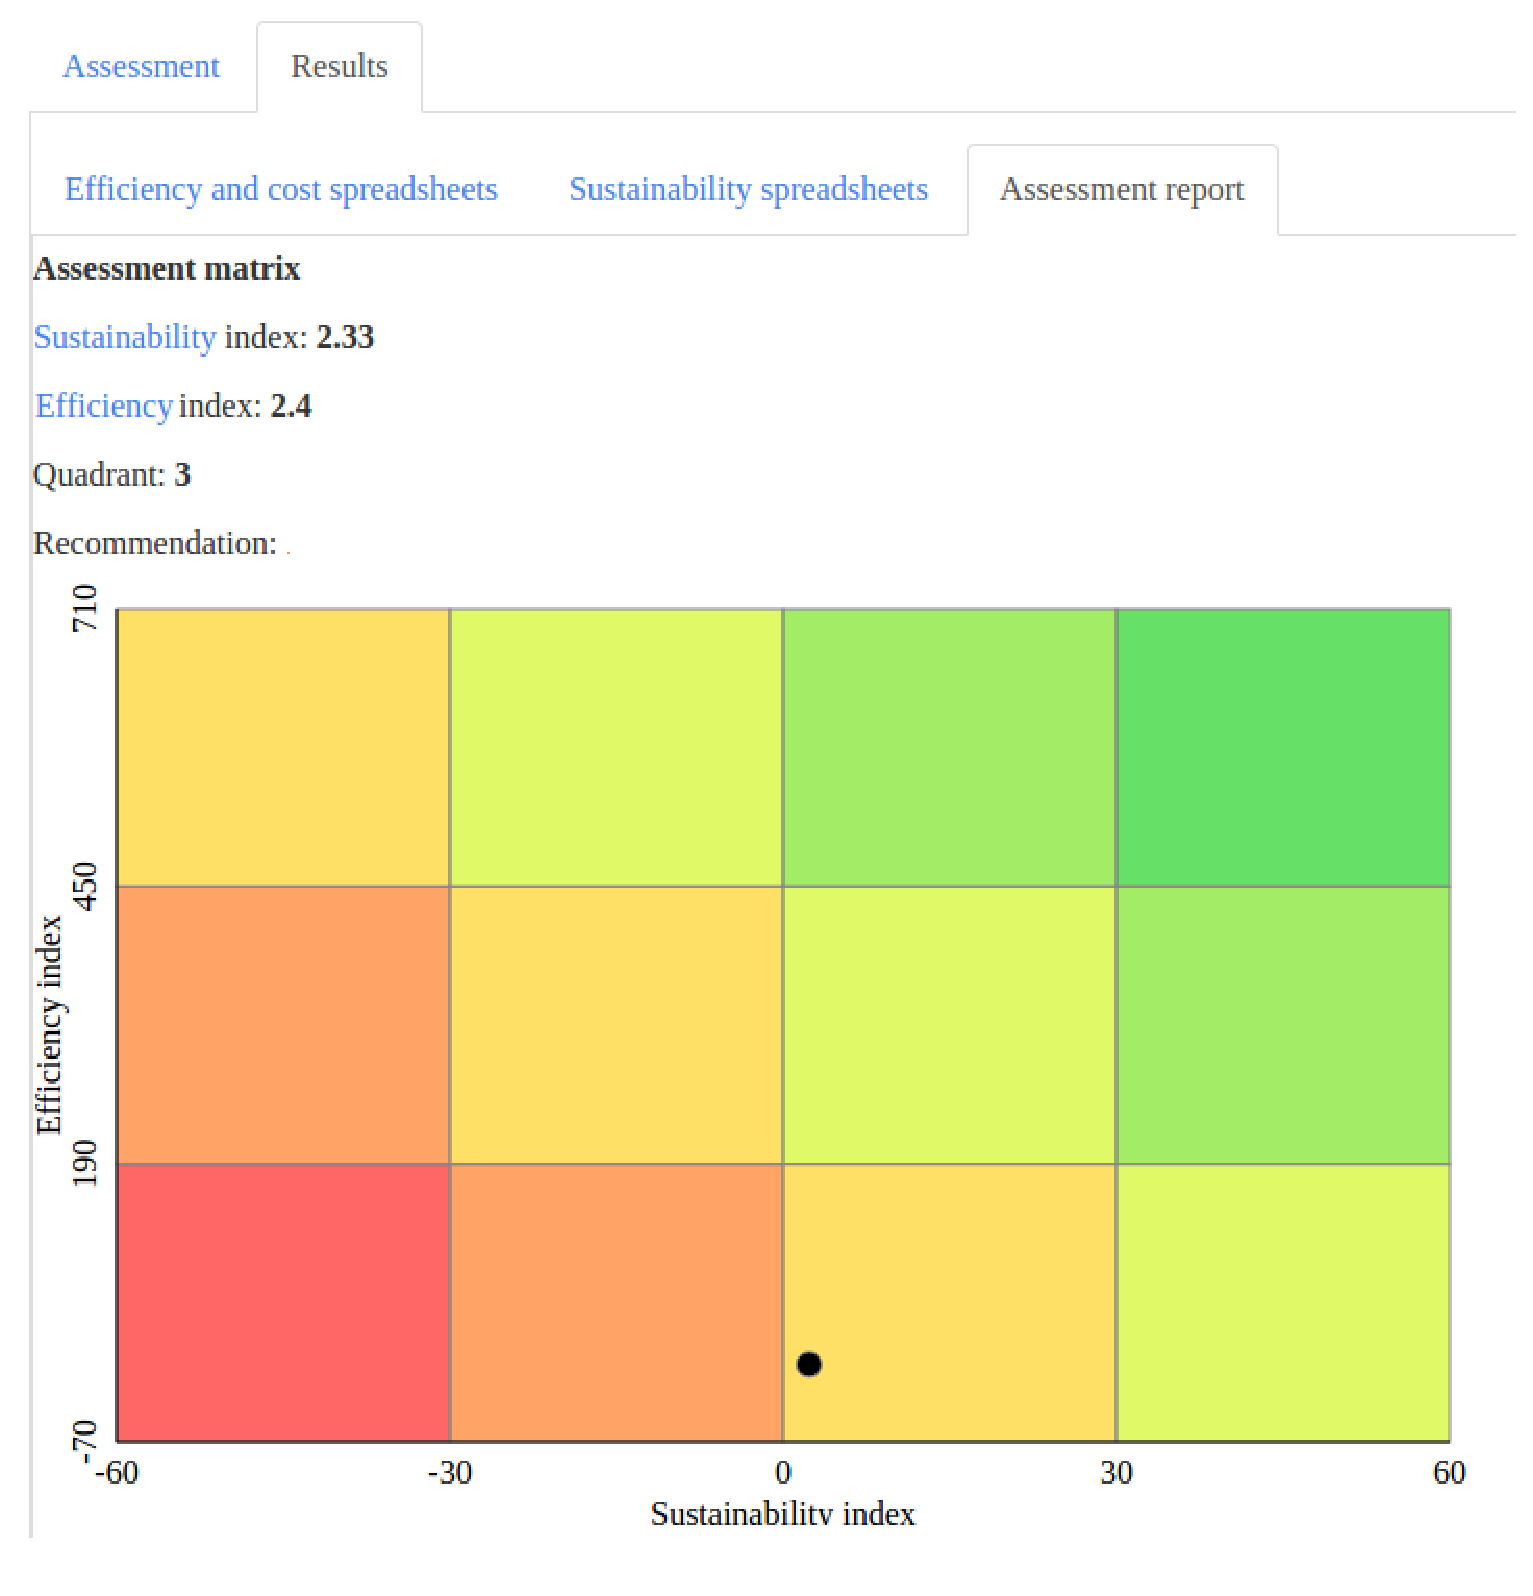
\includegraphics[width=1\columnwidth]{figures/SustenAgro-matrix}
\par\end{centering}
\caption{Matriz de sustentabilidade\label{fig:Matriz-de-sustentabilidade-widget}}
\end{figure}


\subsection*{Semáforo da Sustentabilidade}

O \foreignlanguage{english}{Web Component} do Semáforo da Sustentabilidade
foi o segundo componente para geração de relatórios, no formato definido
pelos especialistas do domínio, desenvolvido para o método SustenAgro.
Ele tem um eixo que quantifica o valor da sustentabilidade normalizado
entre -100 até +100, dividindo o intervalo em 5 segmentos que correspondem
às categorias de sustentabilidade. 

A Figura \ref{fig:Sem=0000E1foro-de-sustentabilidade} mostra esse
componente no sistema SustenAgro com os valores para de avaliação
de sustentabilidade que gerou um índice de sustentabilidade geral
de 4 em escala de -100 até +100.

\begin{figure}[H]
\noindent \begin{centering}
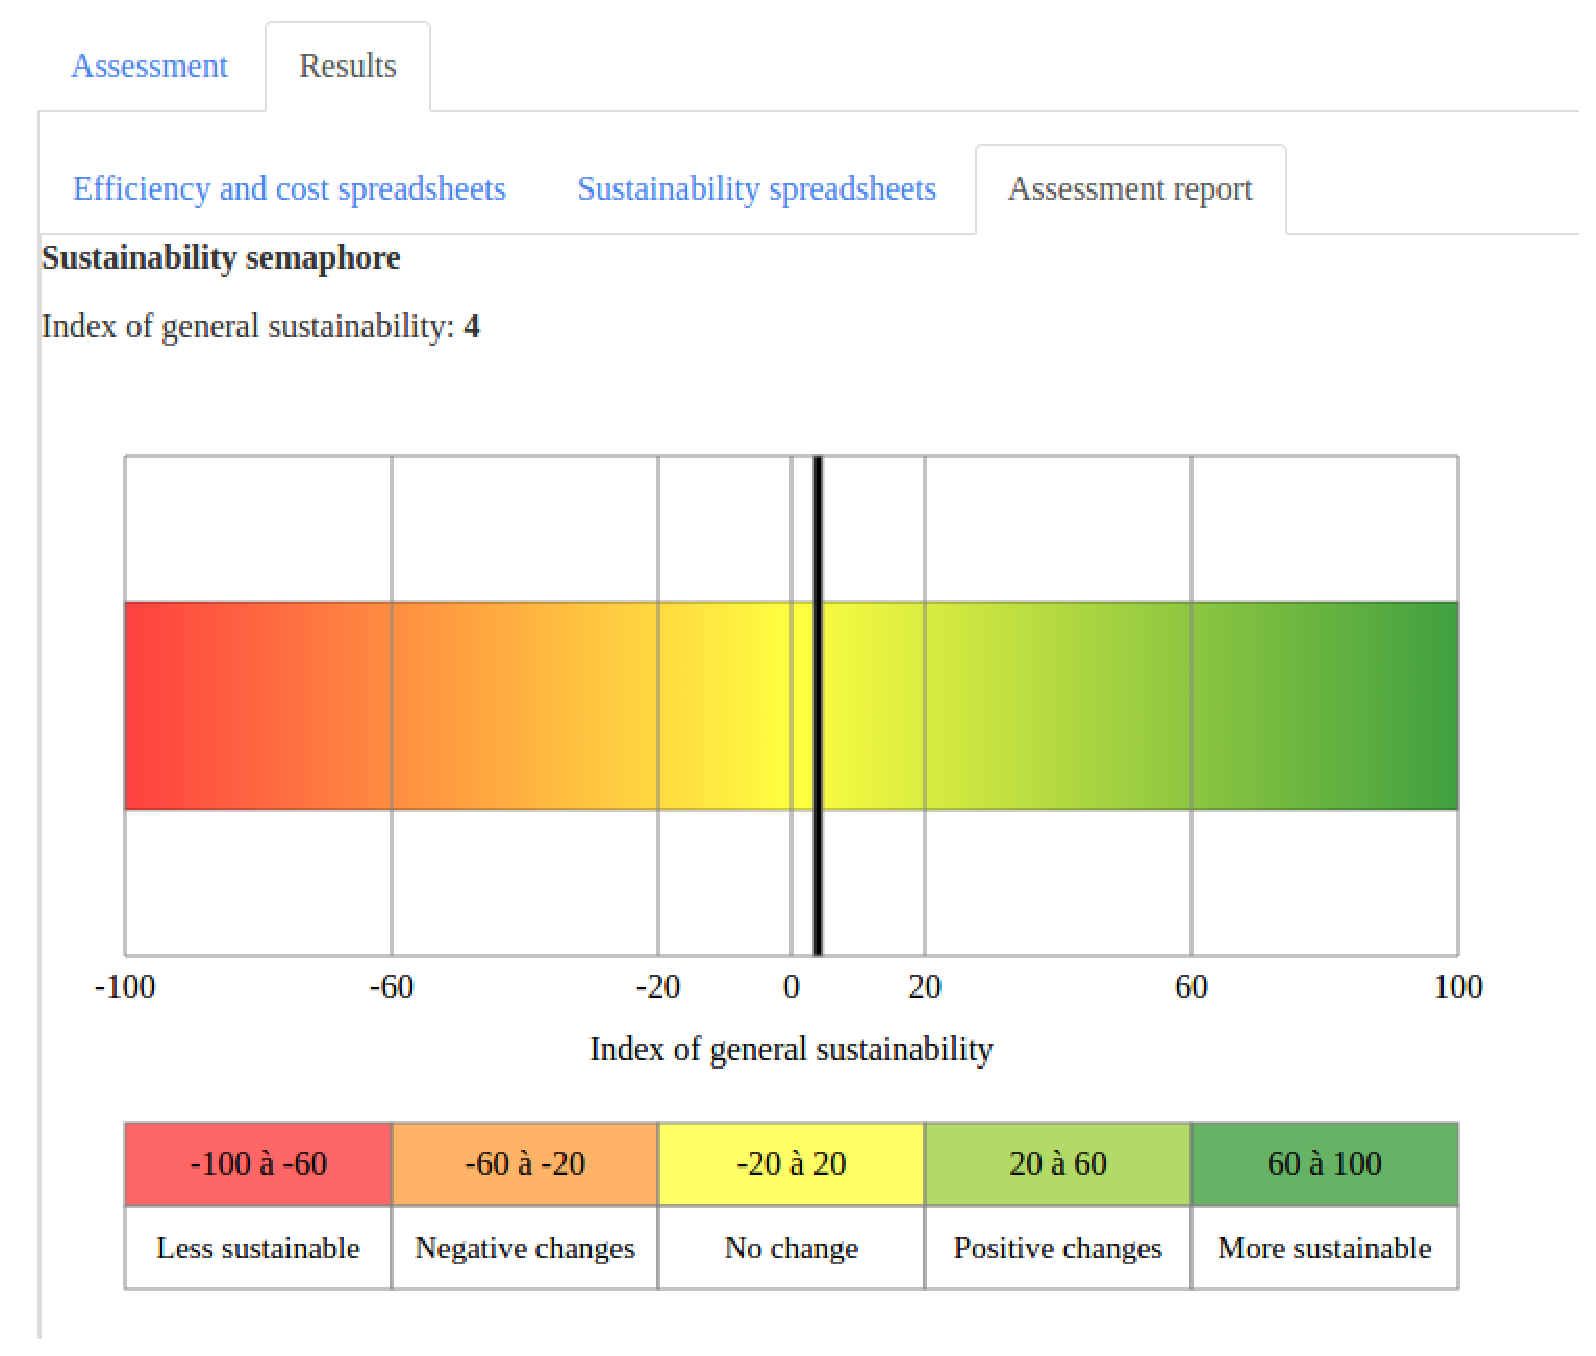
\includegraphics[width=1\columnwidth]{figures/SustenAgro-semaphore}
\par\end{centering}
\caption{Semáforo de sustentabilidade \label{fig:Sem=0000E1foro-de-sustentabilidade}}

\end{figure}

\selectlanguage{english}%

\section{DSL: code}

\selectlanguage{brazil}%
A implementação de uma DSL permite aos especialistas do domínio definir
como são usados e apresentados os conceitos da ontologia, por meio
de elementos da interface gráfica, como os índices de sustentabilidade
serão calculados e quais os elementos presentes no relatório final.
A DSL permite a criação de SADs facilmente adaptáveis às mudanças
do domínio. Os próprios especialistas podem modificá-la sem o auxílio
de programadores.

Para definir o comportamento do SustenAgro, especialistas tiveram
que:

\subsection{Definir o Objeto da Avaliação}

No comando, a seguir \ref{alg:DSL-EvaluationObject} , o Objeto de
Avaliação é definido como uma instância da classe ProductionUnit.
Essa classe foi definida pelos próprios especialistas na ontologia
e tem como filhos as classes \foreignlanguage{english}{\emph{Farm}}
e \foreignlanguage{english}{\emph{Power Plant}} . Também são declaradas
todas as propriedades que os usuários terão que preencher quando criarem
uma avaliação. Por exemplo, na propriedade \textit{hasName} os usuários
devem preencher o nome da unidade de produção.

\begin{algorithm}[H]
\inputencoding{latin9}\begin{lstlisting}[breaklines=true]
evaluationObject ':ProductionUnit', {             
  instance 'ui:hasName', label: ['en': 'Production unit or farm name', 'pt': 'Nome da unidade produtiva ou fazenda']
  instance ':hasAgriculturalProductionSystem', label: ['en': 'Agricultural production system' , 'pt': "Sistema de produ��o agr�cola"]   
  type label: ['en': "Production unit type", 'pt': "Tipo da unidade produtiva"]
  instance  ':hasSugarcaneSource', label: ['en': 'Sugarcane source', 'pt': "Origem da cana"], multipleSelection: true, required: true
  instance 'dbp:state', label: ['en': 'State', 'pt': 'Estado']
  instance 'ui:hasMicroregion', label: ['en': 'Production unit microregion', 'pt': "Microrregi�o da unidade produtiva"]
  instance ':hasAvailabilityOfEvaluationResults', label: ['en': "Availability of evaluation results", 'pt': "Disponibiliza��o dos resultados da avalia��o"]
}
\end{lstlisting}
\inputencoding{utf8}
\caption{DSL que define o Evaluation Object \label{alg:DSL-EvaluationObject}}

\end{algorithm}


\subsection{Definir as características a serem avaliadas}

Agora os especialistas têm que escolher quais características (Features)
dos Objetos de Avaliação serão usadas. No comando \textit{feature},
são indicadas as classes das \textit{Features} a serem usadas. Serão
mostradas todas as \textit{features} das classes indicadas e de suas
descendentes. Por exemplo, o comando \textit{feature ':ProductionEfficiencyFeature'}
vai mostrar todas as \textit{Features} relacionadas com eficiência
da produção. Na ontologia SustenAgro foram estabelecidas as famílias
de \foreignlanguage{english}{\textit{Features}}: EnvironmentalIndicator,
EconomicIndicator, SocialIndicator, ProductionEfficiencyFeature e
TechnologicalEfficiencyFeature.

O comando \textit{feature} também permite dizer se existirão novas
\textit{Features} criadas pelos usuários ('extraFeatures': true) e
a apresentação condicional de grupos de Features. No exemplo do algoritmo
\ref{alg:DSL-Defini=0000E7=0000E3o-de-Features} , são mostradas
Features industriais apenas à usuários de usinas.

\begin{algorithm}
\inputencoding{latin9}\begin{lstlisting}[breaklines=true]
feature ':EnvironmentalIndicator', 'extraFeatures': true 
feature ':EconomicIndicator', 'extraFeatures': true 
feature ':SocialIndicator', 'extraFeatures': true 
feature ':ProductionEfficiencyFeature' 
feature ':TechnologicalEfficiencyFeature', {          
  conditional ":ProductionUnit", 'http://dbpedia.org/ontology/Provider', {
    include ':TechnologicalEfficiencyInTheField'          
  }
  conditional ":ProductionUnit", 'http://dbpedia.org/resource/PhysicalPlant', {
    include ':TechnologicalEfficiencyInTheField', ':TechnologicalEfficiencyInTheIndustrial'          
  }  
}
\end{lstlisting}
\inputencoding{utf8}
\caption{Definição de \foreignlanguage{english}{Features \label{alg:DSL-Defini=0000E7=0000E3o-de-Features}}}

\end{algorithm}


\subsection{Definir o modelamento e a forma de apresentação dos resultados}

Finalmente, no comando \textit{data}, os especialistas definem o nome
da variável que contém as respostas dos usuários e, no comando \textit{report},
fazem o cálculo do modelamento e definem o que vai ser apresentado.
No algoritmo \ref{alg:SustenAgro-DSL} , é possível ver o cálculo
dos índices de sustentabilidade e eficiência através das formulas
do modelo usado pelo SustenAgro. É possível usar qualquer comando
da linguagem Groovy ou biblioteca externa. As variáveis guardam os
valores de interesse que serão mostrados no relatório de avaliação.
No caso do SustenAgro, a variável \foreignlanguage{english}{\textit{sustainability}}
guarda o índice de sustentabilidade e a variável \textit{efficiency}
guarda o índice de eficiência do sistema.

No relatório aparecerão a Matriz de Sustentabilidade (SustainabilityMatrix),
o Semáforo de Sustentabilidade (SustainabilitySemaphore), o texto
\textquotedbl{}Mapa da Microregião\textquotedbl{} e o mapa da microregião
(onde a unidade produtiva se encontra). Cada uma dessas widget é instanciada
na DSL e os valores de interesse são passados para os Web Components
encarregados da apresentação. O framework Decisioner delega aos Web
Components a tarefa de apresentação.

Usuários podem pedir a geração de relatórios em pdf, uma ferramenta
de conversão de HTML para pdf é usada.

\begin{algorithm}[H]
\inputencoding{latin9}\begin{lstlisting}[breaklines=true]
data 'data'
report {       
  environment =   weightedSum(data.':EnvironmentalIndicator')
  economic    =   weightedSum(data.':EconomicIndicator')     
  social      =   weightedSum(data.':SocialIndicator')  
  
  sustainability = (environment + social + economic)/3

  cost_production_efficiency = sum(data.':ProductionEfficiencyFeature')
  technologicalEfficiencyInTheField = 0.8*weightedSum(data.':TechnologicalEfficiencyInTheField')
  technologicalEfficiencyInTheIndustrial = 0.2*weightedSum(data.':TechnologicalEfficiencyInTheIndustrial')

  efficiency = Math.abs(cost_production_efficiency) * (technologicalEfficiencyInTheField+technologicalEfficiencyInTheIndustrial)

  sustainabilityMatrix x: sustainability, y: efficiency,  
                       label_x: ['en': 'Sustainability Index', 'pt': '�ndice de Sustentabilidade'],                 
                       label_y: ['en': 'Efficiency index', 'pt': '�ndice de Efici�ncia'],
                       range_x: [-43,43],
                       range_y: [-160,800],
                       quadrants: [4,3]                       
   
  sustainabilitySemaphore value: sustainability,                  
                          label: ['en': 'Sustainability Level', 'pt': '�ndice da sustentabilidade geral'],
                          range: [-60,60]    

  text 'en': 'Microregion map', 'pt': '**Mapa da microregi�o**'    

  map data.'Microregion'   
}
\end{lstlisting}
\inputencoding{utf8}
\caption{SustenAgro DSL \label{alg:SustenAgro-DSL}}

\end{algorithm}


\section{Considerações Finais}

O desenvolvimento do sistema Sustenagro satisfez uma necessidade presente
na unidade da Embrapa Meio Ambiente: um sistema de avaliação de sustentabilidade
em cana-de-açúcar no centro-sul do Brasil. O SAD SustenAgro representa
e permite complementar informações e dados do estado atual de sustentabilidade
nas fazendas e usinas. Ele produz relatórios com a finalidade de embasar
e formalizar políticas para promover práticas produtivas mais sustentáveis,
de acordo com critérios ambientais, sociais e econômicos.

Além de satisfazer uma necessidade institucional, o SustenAgro é uma
proposta de SAD baseado em conhecimento e vinculado às tecnologias
da web semântica. O SustenAgro não foi apenas uma instanciação do
framework Decisioner, ele definiu o próprio framework. Através do
desenvolvimento do SustenAgro, foi possível determinar as características
gerais desse tipo de SAD, e implementá-las no framework, e as características
específicas do Sustenagro, que foram implementadas usando a ontologia
SustenAgro, os dois Web Components e a DSL.

Tendo o sistema SustenAgro instanciado e rodando, foi possível validar
suas funcionalidades através de alguns experimentos com integrantes
do projeto SustenAgro da Embrapa. Os resultados obtidos nas avaliações
dos experimentos serão detalhados no próximo capítulo.


\chapter{Avaliação\label{chap:Avalia=0000E7=0000E3o}}

O SAD SustenAgro (capítulo \ref{chap:SustenAgro}) foi instanciado
usando o Framework Decisioner (capítulo \ref{chap:Decisioner}) e
avaliado, durante diferentes estágios de desenvolvimento, através
de experimentos realizados com especialistas de domínio e usuários
da Embrapa. Esses dois sistemas foram desenvolvidos com metodologias
iterativas, onde foram realizadas varias inspeções e testes durante
a implementação. Uma avaliação final também foi realizada para analisar
se as funcionalidades foram implementadas corretamente.

A seguir, são apresentadas as avaliações realizadas no SAD SustenAgro
e ao Framework Decisioner. Elas foram independentes e geraram resultados
que levaram ao redesenho das arquiteturas de ambos sistemas em diferentes
etapas do seu desenvolvimento.

\section{Avaliação das Web UI.}

Na finalização do processo de design das Web UI, explicado na Seção
\ref{sec:Web-UI}, foi realizada uma avaliação da usabilidade das
mesmas no SAD SustenAgro. Os detalhes dessa avaliação foram:
\begin{description}
\item [{Data}] Junho de 2015
\item [{Participantes}] Usuários da ferramenta: especialista em sustentabilidade
e especialista em economia agrícola
\item [{Local}] Instituto de Ciências Matemáticas e de Computação (ICMC-USP)\nomenclature{ICMC}{ Instituto de Ciências Matemáticas e de Computação} 
\item [{Técnica}] Avaliação de usabilidade
\end{description}
Nesta avaliação foi apresentado, aos usuários especialistas em sustentabilidade,
o processo de design da UI e o protótipo da interface gráfica de usuário
do SAD SustenAgro sem dados reais. Nessas interfaces, eles interagiram
com as telas, através de um navegador web, fazendo uso das funcionalidades
do SAD que simulava os dados durante o processo.

Durante esta avaliação foram verificados, os três aspectos da usabilidade:
\begin{itemize}
\item Eficácia: as interfaces permitiram realizar as tarefas segundo as
funcionalidades definidas e permitiam interagir de maneira intuitiva
para realizar as tarefas.
\item Eficiência: o aceso à ferramenta foi realizado em tempos esperados
e foi possível realizar as tarefas com recursos típicos de um laptop
e um navegador web.
\item Satisfação: os usuários conseguiram realizar as tarefas sem problemas
e com uma experiência de fácil uso, onde a ferramenta fornecia informação
de ajuda para realizar as interações.
\end{itemize}
A avaliação foi positiva, cumprindo os três requisitos anteriores
de usabilidade. Esta avaliação gerou várias recomendações para melhorar
a interface gráfica de usuário, entre elas as mais relevantes foram: 
\begin{itemize}
\item Mudar a organização do processo de avaliação, agrupando varias tarefas
em uma seção denominada ``caracterização da unidade produtiva'',
que permite definir a localização, as principais características e
a disponibilização da informação em um processo unificado. 
\item Agrupar os resultados em uma seção ``Resultados'', integrando os
\foreignlanguage{english}{Web Components} específicos do SustenAgro
com os resultados da avaliação.
\item Organizar os indicadores em uma hierarquia simplificada que facilita
o preenchimento dos mesmos.
\end{itemize}
Depois de implementar as recomendações anteriores, foi continuado
o desenvolvimento com a integração da ontologia SustenAgro e da DSL.
Foi necessário realizar ajustes da interface ao integrar cada funcionalidade.
As principais mudanças foram realizadas devido a esta avaliação.

\section{Avaliação da ontologia de domínio de avaliação da sustentabilidade.}

A ontologia SustenAgro foi o resultado da modelagem do conhecimento
dos especialistas, que passou por várias etapas, desde ser definida
em texto, modelada em mapas conceituas e criada a ontologia em \foreignlanguage{english}{OWL}
(esse processo foi detalhado na Seção \ref{sec:Metodologia}). Cada
uma dessas etapas requereu inspeções por parte dos especialistas para
verificar a correta modelagem, uma avaliação formal foi realizada
e os detalhes são descritos a seguir.
\begin{description}
\item [{Data}] 14 de abril do 2016
\item [{Participantes}] Especialista em sustentabilidade e especialista
em modelagem de conhecimento
\item [{Local}] Embrapa Informática Agropecuária - Campinas
\item [{Técnica}] Visualização da ontologia e recuperação de conhecimento
\end{description}
O especialista em modelagem de conhecimento da Embrapa Informática
Agropecuária e o especialista em sustentabilidade reuniram-se para
realizar a revisão da ontologia SustenAgro por meio de ferramentas
de engenharia de conhecimento que permitiram visualizar as ontologias.

As ferramentas usadas na avaliação foram yWorks \footnote{\url{http://www.yworks.com/}}
e Gephi \footnote{\url{https://gephi.org/}}. Elas representaram aspectos
da ontologia usando diversas visualizações de grafos, permitindo avaliar
a coerência das conexões entre os nós daqueles grafos.

Também foi analisado o SAD SustenAgro, que tinha a ontologia integrada,
usando as funcionalidades que requeriam dados da ontologia, verificando
a informação recuperada e a coerência dela em relação à existente
na ontologia. 

A reunião de avaliação chegou no consenso: a ontologia \foreignlanguage{english}{OWL}
está representando a avaliação da sustentabilidade do sistema de produção
de cana no centro-sul do Brasil, destacando a especificidade dela
para suportar o SAD Sustenagro e que seu foco em conceitos concretos.

Foi recomendado integrar outros tipos de visualizações e editores
de ontologia no framework Decisioner. Entre eles foi recomendado fornecer
um editor visual de ontologias, basado na ferramenta \foreignlanguage{english}{WebVOWL,}
definida e desenvolvida por \citet{lohmann2014webvowl}. Devido a
limitações de tempo, não foi possível a implementação dessa sugestão
específica.

\section{Avaliação do protótipo funcional com dados}

Com a finalidade de avaliar a implementação do método SustenAgro,
foram realizados testes de vários tipos de avaliações, para comparar
com resultados de outras fontes, e assim validar a correta implementação.
Os detalhes da avaliação foram.
\begin{description}
\item [{Data}] 6 de junho do 2016
\item [{Participantes}] Especialista em sustentabilidade e especialista
em economia agrícola
\item [{Local}] Agência Paulista de Tecnologia dos Agronegócios (APTA)
\item [{Técnica}] Testes numéricos dos resultados do software
\end{description}
A revisão dos resultados numéricos foi realizada a partir de vários
cenários de indicadores, sendo realizada uma comparação dos resultados
processados manualmente com os resultados de avaliação do SAD SustenAgro.
Os resultados manuais foram iguais aos calculados pelo sistema, o
que permitiu validar a correta definição do método SustenAgro e sua
implementação no SAD SustenAgro. 

Os cenários avaliados foram casos extremos dos indicadores, processo
denominado teste de mínimos e máximos, gerando resultados em forma
de relatório para cada um dos cenários. A Figura \ref{fig:Matriz-de-sustentabilidade-Maximos}
apresenta a Matriz de Sustentabilidade com o cenário de mínimos, na
qual o ponto preto identifica o resultado da avaliação. Ele ficou
no primeiro quadrante tal como se esperava. Os resultados para testes
de máximos também se comportaram como esperado.

\begin{figure}[H]
\begin{centering}
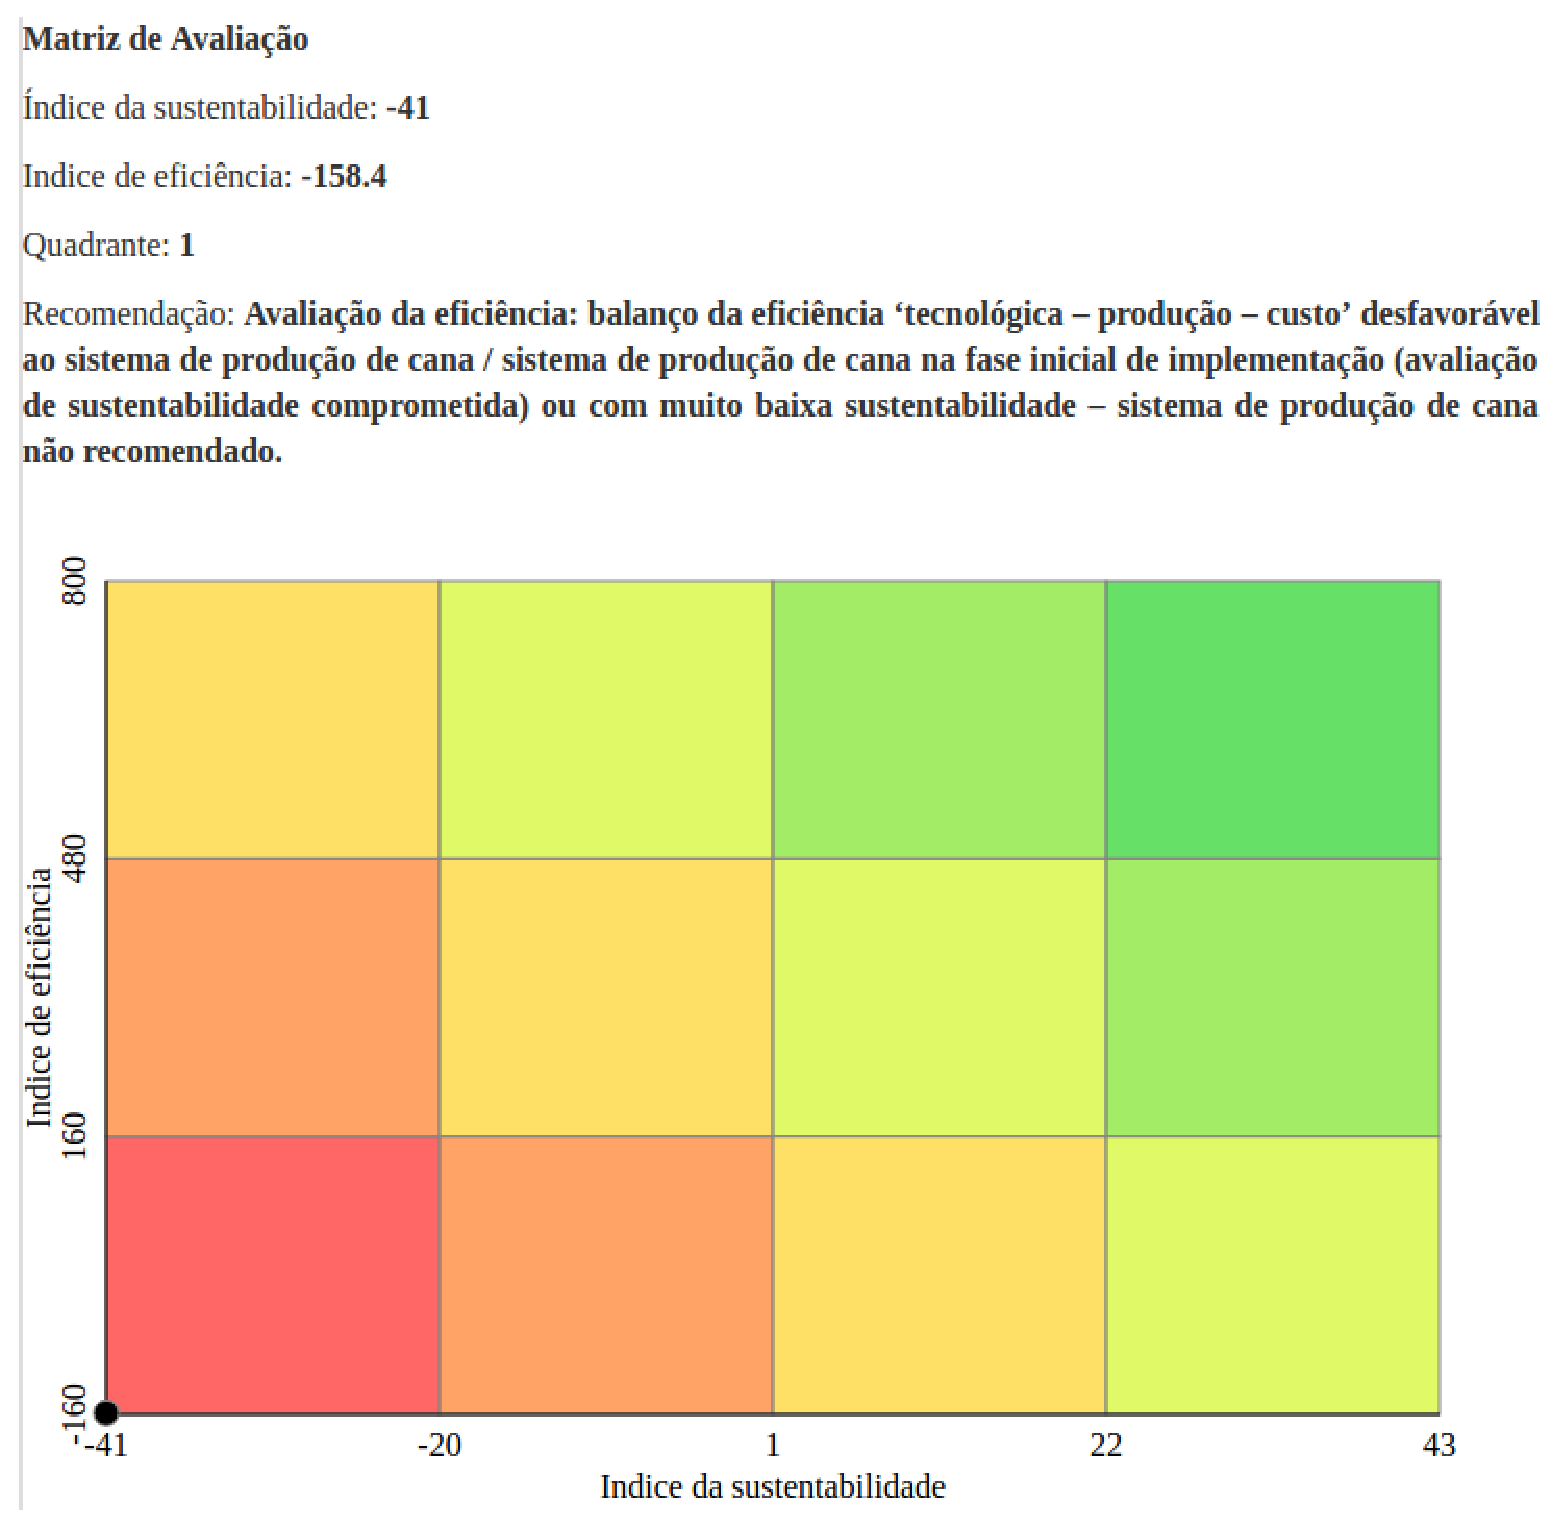
\includegraphics[width=0.8\columnwidth]{figures/Minimum}
\par\end{centering}
\caption{Matriz de Sustentabilidade com valores mínimos.\label{fig:Matriz-de-sustentabilidade-Maximos}}

\end{figure}

Um dos aspectos importantes da ferramenta, é que ela permite que os
próprios especialistas mudem, em tempo real, as fórmulas do método
de avaliação, permitindo fazer ajustes finos no método. Essa funcionalidade
permitiu descobrir e avaliar rapidamente um problema do método original:
a integração de uma operação de valor de um valor absoluto na fórmula.
A possibilidade da interação direta e fácil dos especialistas, em
tempo real, com o sistema permitiu demostrar agilmente possíveis cenários
de resolução do problema e aceitar rapidamente uma solução, proposta
pelo autor.

\section{Avaliação do SAD SustenAgro e do Framework Decisioner: }

A partir da avaliação da ontologia, da implementação do método SustenAgro
e do desenvolvimento das Web UI realizou-se uma avaliação do SAD com
a finalidade de avaliar a integração desses componentes.
\begin{description}
\item [{Data}] 18 de maio do 2016 até o dia 22 de junho do 2016
\item [{Participantes}] Usuários especialistas e usuários finais.
\item [{Local}] Instituto de Ciências Matemáticas e de Computação (ICMC-USP)
\item [{Técnica}] Teste de usabilidade
\end{description}
Para realizar uma avaliação integral do SAD SustenAgro e do Framework
Decisioner, foi necessário fazer testes de usabilidade com usuários
de ambos os perfis do sistema (especialistas de domínio e usuários
finais). Essa avaliação foi realizada com a maioria dos membros da
equipe SustenAgro e com usuários finais, de maneira remota e independente,
totalizando 8 avaliações.

A avaliação consistiu em realizar um conjunto de tarefas com o SAD
SustenAgro v1.0 e responder se foi possível terminar a tarefa e as
sugestões. As tarefas e perguntas solicitadas aos usuários estão listadas
no Apêndice \ref{sec:Formul=0000E1rio-de-avalia=0000E7=0000E3o-SustenAgro}
e permitiram gerar os seguintes resultados das avaliações:

\begin{longtable}{|>{\centering}p{0.2\columnwidth}|>{\centering}p{0.2\columnwidth}|>{\centering}p{0.6\columnwidth}|}
\hline 
\textbf{\small{}Perfil de Usuário} & \textbf{\small{}Avaliação} & \textbf{\small{}Sugestões}\tabularnewline
\hline 
\hline 
{\small{}Usuário final 1} & {\small{}Positiva, realizou as 5 tarefas de usuário final com sucesso} & \begin{itemize}
\item {\small{}Aumentar a ajuda para cada funcionalidade}{\small \par}
\item {\small{}Barra de progresso durante a avaliação}{\small \par}
\item {\small{}Resultados de avaliação mais detalhados}
\end{itemize}
\tabularnewline
\hline 
\hline 
{\small{}Usuário final 2} & {\small{}Positiva, realizou as 5 tarefas de usuário final com sucesso} & \begin{itemize}
\item {\small{}Melhorar a explicação do processo de avaliação}{\small \par}
\item {\small{}Resultados numéricos com formatação }
\end{itemize}
\tabularnewline
\hline 
\hline 
{\small{}Usuário final 3} & {\small{}Positiva, realizou as 5 tarefas de usuário final com sucesso} & \begin{itemize}
\item {\small{}Segurança no cadastro da senha}{\small \par}
\item {\small{}Melhorar a localização do botão avaliar}{\small \par}
\item {\small{}Remover }\foreignlanguage{english}{{\small{}scroll}}{\small{}
externo}{\small \par}
\item {\small{}Salvar automaticamente os dados}
\end{itemize}
\tabularnewline
\hline 
\hline 
{\small{}Especialista em sustentabilidade} & {\small{}Positiva, realizou as 5 tarefas de usuário e as 5 tarefas
de especialista de domínio com sucesso} & \begin{itemize}
\item {\small{}Definir e acrescentar os termos de uso}{\small \par}
\item {\small{}Melhorar a sequencia de telas durante o cadastro de novo
usuário}{\small \par}
\item {\small{}Balão explicativo dos campos do formulário de nova unidade
produtiva, especificamente a propriedade de publicação dos dados}{\small \par}
\item {\small{}Definir o limite de caráteres para o campo de justificativa}{\small \par}
\item {\small{}Salvar avaliação ao mudar de aba}{\small \par}
\item {\small{}Justificativas sempre visíveis na tela de resultados.}{\small \par}
\item {\small{}Acrescentar bandeira em inglês e termos de uso}
\end{itemize}
\tabularnewline
\hline 
\hline 
{\small{}Especialista economia} & {\small{}Positiva, realizou as 5 tarefas de usuário e as 5 tarefas
de especialista de domínio com sucesso} & \begin{itemize}
\item {\small{}Salvar dados da seção automaticamente}{\small \par}
\item {\small{}Mudanças em alguns }\foreignlanguage{english}{{\small{}labels}}{\small \par}
\item {\small{}Mudanças nos indicadores}{\small \par}
\item {\small{}Componentes gráficos para representar os dados }{\small \par}
\item {\small{}Editor visual de ontologia e internacionalização}
\end{itemize}
\tabularnewline
\hline 
\hline 
{\small{}Especialista em ontologias} & {\small{}Positiva, realizou as 5 tarefas de usuário final com sucesso} & \begin{itemize}
\item {\small{}Melhorar a apresentação do botão salvar}{\small \par}
\item {\small{}Indicadores em forma de pergunta com verbo e simbolo de pergunta}{\small \par}
\item {\small{}Informar a possibilidade de edição de indicadores }
\end{itemize}
\tabularnewline
\hline 
\hline 
{\small{}Especialista agricultura} & {\small{}Positiva, realizou as 5 tarefas de usuário final com sucesso} & \begin{itemize}
\item {\small{}Cadastrar mais de uma microrregião}{\small \par}
\item {\small{}Remover }\foreignlanguage{english}{{\small{}scroll}}{\small{}
externo, mudanças em vários indicadores}{\small \par}
\item {\small{}Melhorar a localização do botão salvar e avaliar}{\small \par}
\item {\small{}Salvar a seção para não perder os dados}{\small \par}
\item {\small{}Melhorar a apresentação do pdf}
\end{itemize}
\tabularnewline
\hline 
\hline 
{\small{}Especialista em computação} & {\small{}Positiva, realizou as 5 tarefas de usuário final com sucesso} & \begin{itemize}
\item {\small{}Salvar a seção e os dados dela em tempo real}{\small \par}
\item {\small{}Integrar sistemas externos para poupar informação (caracterização
da unidade produtiva) }
\end{itemize}
\tabularnewline
\hline 
\end{longtable}

\begin{table}[H]
\caption{Avaliação do SAD SustenAgro}
\end{table}

A partir dessa avaliação integral, feita por usuários finais e administradores,
foram definidas várias melhorias a serem realizadas no Framework Decisioner
e o SAD SustenAgro. Devido às limitações de tempo e de desenvolvedores,
foram implementados apenas os ajustes visuais nas web UI, melhoras
na apresentação dos resultados, na geração do PDF e, principalmente,
a inclusão da linguagem inglês. Essa última mudança foi selecionada
como de especial importância, por parte dos especialistas. Neste documento,
são apresentadas várias telas, tanto em português como em inglês,
que foram geradas a partir da implementação dessa funcionalidade.
\selectlanguage{english}%

\section{Workshop\foreignlanguage{brazil}{: validação do software SustenAgro
v1.0 com equipe de especialistas.}}

\selectlanguage{brazil}%
A partir das melhoras realizadas na avaliação interna pelos dois tipos
de usuários do SAD SustenAgro, o sistema foi disponibilizado em servidos
web do ICMC. Esta publicação permitiu dar suporte a uma avaliação
no formato de \foreignlanguage{english}{workshop} com especialistas
de diversos perfis que tinham interesse no SAD SustenAgro. O \foreignlanguage{english}{Workshop}
foi intitulado ``Validação do software SustenAgro'', os detalhes
do \foreignlanguage{english}{workshop} são apresentados a seguir.
\begin{description}
\item [{Data}] 14 de julho do 2016
\item [{Participantes}] Equipe do projeto SustenAgro de várias unidades
da Embrapa
\item [{Local}] Embrapa Informática Agropecuária - Campinas
\item [{Técnica}] Delphi
\end{description}
O \foreignlanguage{english}{workshop} teve o objetivo de avaliar a
qualidade e acuidade do SAD SustenAgro em termos da clareza da informação
técnica apresentada nas interfaces, com vistas a garantir o entendimento
do usuário e possibilitar que a avaliação da sustentabilidade do sistema
de produção de cana-de-açúcar seja realizada da melhor forma possível. 

No \foreignlanguage{english}{workshop} foi apresentado o formulário
de avaliação (Seção \ref{sec:Formulario-Delphi-Workshop}) usando
a técnica \foreignlanguage{english}{Delphi} \citep{wright1985tecnica},
a um grupo de especialistas com perfis de varias áreas do conhecimento,
entre eles destacam-se:
\begin{itemize}
\item Especialista em sustentabilidade
\item Especialista em ciências agrícolas
\item Especialista em modelagem de conhecimento
\item Especialista em ciência e Tecnologia do Bioetanol
\item Especialista em ciências da computação
\item Especialista em economia agrícola
\item Especialista em biotecnologia
\item Mestrando em ciências da computação (sistemas web e multimídia)
\item Mestrando em Planejamento de Sistemas Energéticos
\end{itemize}
As interações com o sistema foram filmadas enquanto os usuários executavam
uma lista de tarefas. Monitores do ICMC ficavam estimulando os usuários
a falar o que estavam pensando (técnica Think Aloud ) e os questionavam,
quando tinham alguma dificuldade de interação. Ao final, houve um
\foreignlanguage{english}{debriefing} e foram também colhidas mais
sugestões de mudança. 

Os especialistas aprovaram a ferramenta tanto na interação como no
conteúdo dela, com as seguintes sugestões:
\begin{itemize}
\item As perguntas dos indicadores não são de fácil interpretação.
\item Colocar mais informações na interface para facilitar o uso dela, por
exemplo o significado de alinhamento dos indicadores.
\item Alguns indicadores estão repetidos.
\item Os resultados da avaliação deveriam estar por dimensão.
\item Demora para salvar os dados inseridos.
\item A informação dos site tem inconsistências em relação à informação
do pdf gerado.
\item A recomendações do relatório precisam mais detalhamento.
\end{itemize}
É interessante que muitas das sugestões não tem haver com aspectos
computacionais ou de interface, mas sim com o processo de avaliação
de sustentabilidade. Esse processo é de inteira responsabilidade dos
especialistas de domínio (e foge totalmente do escopo deste trabalho).
Isso foi um ponto positivo. É natural que especialistas em sustentabilidade
estejam muito mais interessados na sua área do que nos aspectos computacionais
do SAD SustenAgro. Uma boa interface é aquela que desaparece da mente
do usuário e permite que este se foque na sua tarefa. Neste caso,
a avaliação de sustentabilidade. Acreditamos que o SAD SustenAgro
atendeu bem a esse requisito.

\section{Avaliação de SAD SustenAgro nos servidores da Embrapa}

A partir da aprovação do SAD SustenAgro, por parte dos especialistas
no \foreignlanguage{english}{workshop}, foi autorizada a instalação
da ferramenta nos servidores da Embrapa Meio Ambiente. Essa instalação
foi um esforço coordenado entre o desenvolvedor do framework Decisioner
(o autor deste trabalho) e técnicos de informática da Embrapa.
\begin{description}
\item [{Data}] 18 de agosto do 2016
\item [{Participantes}] Especialista em Sustentabilidade e especialista
em TI
\item [{Local}] Embrapa Meio Ambiente - Campinas
\item [{Técnica}] Teste de usabilidade
\end{description}
A instalação, coordenada pelo desenvolvedor do Framework Decisioner
e técnicos da Embrapa, foi problemática. A Embrapa não autoriza o
acesso físico ou via ssh aos servidor por parte de profissionais externos.
Por esta razão, foi criado um documento de instalação, descrito no
Apêndice \ref{chap:Instalation}. Nele estão as instruções para instalar
o Framework Decisioner e instanciar o SAD SustenAgro.

A instalação foi exitosa e o sistema está funcionando no endereço
\url{https://sustenagro.embrapa.br/}. Atualmente o endereço não está
no ar, pois o SAD SustenAgro está em processo de registro no Instituto
Nacional de Propriedade Intelectual (INPI), em nome da Embrapa e USP,
e a Embrapa ter uma política de exigir esse registro para liberação
para uso externo.

\section{Conclusões}

Essas avaliações permitiram verificar que os requisitos do Framework
Decisioner e do SAD SustenAgro foram implementados corretamente e
que atenderam as necessidades dos especialistas de domínio e usuários
finais, identificadas nos levantamentos de requisitos.

As avaliações ocorreram em diferentes fases do projeto e cada uma
trouxe correções e melhoras que foram implementadas, na medida do
possível, segundo a relevância de cada mudança e o tempo disponível
para desenvolvedor do projeto. Por ter sido desenvolvido em um processo
cíclico, cada iteração acrescentou novas funcionalidades que fizeram
mudar a arquitetura dos sistemas, gerando \foreignlanguage{english}{bugs}
e inconsistências. Na versão 1.0, os sistemas contam com funcionalidades
estáveis que permitem fornecer os serviços implementados. Correções
e sugestões recebidas durante a avaliação e não implementadas por
problema de tempo, foram deixadas como trabalhos futuros, que serão
apresentados no próximo capítulo juntamente com as conclusões.


\chapter{Conclusões\label{chap:Conclus=0000E3o}}

Os resultados obtidos são: 
\begin{enumerate}
\item Ontologia em formatos da web semântica (RDF/OWL) da avaliação da sustentabilidade
no sistema de cana-de-açúcar. 
\item Protótipo de ontologia de interfaces gráficas em formatos da web semântica
(RDF/OWL) 
\item Linguagem de domínio especifico DSL, Decisioner, para definir e permitir
administrar os parâmetros e processos do sistema SustenAgro 
\item Protótipo de sistema de geração de interfaces suportado nas tecnologias
da web semântica 
\item Formulários para recolha de dados sobre sustentabilidade em cana-de-açúcar,
e o processo de colheita dos dados de algumas usinas do estado de
São Paulo 
\item Protótipo do sistema web Sustenagro que integra as ontologias e a
DSL, fornecendo um comportamento configurável em tempo de execução
dos parâmetros, processos e das interfaces gráficas de usuário
\end{enumerate}
Uma das finalidades deste projeto é construir um gerador de sistemas
de apoio a decisão que consiga suportar outros domínios de conhecimento,
propondo para a comunidade uma metodologia de desenvolvimento e manutenção
que fique simples para os usuários finais e assim permitir que os
especialistas no domínio façam as mudanças sem precisas dos especialistas
de T.I.

\section{Trabalhos Futuros}

Este capítulo apresenta os resultados estão uma versão da ontologia
de domínio do SustenAgro e artefatos para o desenvolvimento da interface
visual do sistema: User Stories, Scenarios, Story Boards, Mockups
e um protótipo para a interface do SustenAgro.

Os resultados obtidos são: 
\begin{enumerate}
\item Ontologia em formatos da web semântica (RDF/OWL) da avaliação da sustentabilidade
no sistema de cana-de-açúcar. 
\item Protótipo de ontologia de interfaces gráficas em formatos da web semântica
(RDF/OWL) 
\item Linguagem de domínio especifico DSL, Decisioner, para definir e permitir
administrar os parâmetros e processos do sistema SustenAgro 
\item Protótipo de sistema de geração de interfaces suportado nas tecnologias
da web semântica 
\item Formulários para recolha de dados sobre sustentabilidade em cana-de-açúcar,
e o processo de colheita dos dados de algumas usinas do estado de
São Paulo 
\item Protótipo do sistema web Sustenagro que integra as ontologias e a
DSL, fornecendo um comportamento configurável em tempo de execução
dos parâmetros, processos e das interfaces gráficas de usuário
\end{enumerate}
Uma das finalidades deste projeto é construir um gerador de sistemas
de apoio a decisão que consiga suportar outros domínios de conhecimento,
propondo para a comunidade uma metodologia de desenvolvimento e manutenção
que fique simples para os usuários finais e assim permitir que os
especialistas no domínio façam as mudanças sem precisas dos especialistas
de T.I.


\bibliographystyle{abntex2-alf}
\bibliography{references/references}


\appendix

\chapter{Método SustenAgro de Avaliação de Sustentabilidade}

\label{chap:Sustainability_Assessment}Este anexo apresenta os principais conceitos relacionados com a avaliação
da sustentabilidade segundo segundo os fines do projeto SustenAgro,
e como foram usados no processo de avaliação de sustentabilidade.

\section{Sustentabilidade}

Não existe um consenso sobre a definição de sustentabilidade, mas
uma definição orientadora para os fins do presente projeto é a seguinte:
\begin{quotation}
``O desenvolvimento sustentável prevê o atendimento das necessidades
do presente sem comprometer a capacidade das gerações futuras de suprir
suas próprias necessidades, \foreignlanguage{english}{Brundtland Commission}''
\citet{Burton:1987,brundtland1987our}
\end{quotation}
Este conceito foi ratificado pela Conferência das Nações Unidas sobre
o Meio Ambiente e Desenvolvimento, a Rio-92 \citet{ehlers1996agricultura}
a Rio+20 \citet{ONU2012}, após do relatório \foreignlanguage{english}{Brundtland}
a ênfase do conceito desloca-se da integridade ambiental para o elemento
humano, gerando um equilíbrio entre as dimensões econômica, social
e ambiental \citet{van2005indicadores}.

\citet{gliessman2001agroecologia} teoriza que não há como encontrar
a sustentabilidade e, portanto, o seu conceito mais representativo,
pois a mesma permanece sempre no futuro, dado o compromisso que os
sistemas têm de garantir as necessidades das gerações futuras. Assim,
a sustentabilidade é algo relativo ao tempo, ou seja, um sistema pode
ser mais ou menos sustentável que outro dependendo do tempo em que
for avaliado e do entendimento da sustentabilidade neste contexto.

A sustentabilidade esta vinculada a vários domínios de conhecimento,
um deles é a sustentabilidade em agricultura, que é de especial interesse
na segurança alimentar. Em 2050 a população mundial atingirá 9.1 bilhões
de pessoas FAO (2013), o qual imporá enormes desafios para garantir
a sustentabilidade em meio do aumento de alimentos, por isso são necessários
incentivos e políticas para garantir a sustentabilidade em agricultura,
a través da geração de estratégias que permitam conhecer o estado
dos sistemas produtivos e melhorar segundo as necessidades identificadas.

Segundo \citet{van2008integrated} os sistemas agrícolas evoluem continuamente
e são afetados por uma gama de forças globais e locais, os aspectos
que mais influenciam na sustentabilidade da agricultura são os tecnológicos
e políticos, permitindo identificar e melhorar diversos aspectos da
produção agrícola. 

Uma estrategia para quantificar a sustentabilidade são a definição
métodos e metodologias de avaliação, as quais utilizam indicadores,
um exemplo deste enfoque é exposto por \citet{AlkanOlsson:2009} que
desenvolveu um \foreignlanguage{english}{\emph{framework}} de indicadores
que relaciona de uma maneira consistente as dimensões ambiental, econômica
e social do desenvolvimento sustentável, seu principal benefício é
uma relativa simplicidade na apresentação da informação e a possibilidade
de vincular os indicadores com objetivos políticos de cada dimensão
da sustentabilidade e assim facilitar a comparação dos impactos das
novas políticas em cada dimensão.

\section{Dimensões da Sustentabilidade}

As dimensões da sustentabilidade são classificações que permitem identificar
e agrupar conceitos de sustentabilidade\citep{AlkanOlsson:2009}.,
dependendo da teoria de sustentabilidade escolhida, existem diversas
propostas de dimensões que podem ser usadas segundo a finalidade da
pesquisa, um exemplo desta classificação é a assumida na pesquisa
de \citet{oliveira:2013} onde são definidas seis dimensões da sustentabilidade:
Ambiental, Social, Agrícola/Industrial, Produtos/Subprodutos, Tecnológica
e Política.

No caso do sistema SustenAgro determinou-se pela equipe de especialistas
em sustentabilidade fazer uma divisão segundo a proposta do Relatório
Brundtland \citep{brundtland1987our}, onde foram identificadas as
três dimensões da sustentabilidade: ambiental, social e econômica,
as quais têm a mesma importância gerando um equilíbrio.

Ditas dimensões são sistemas complexos que integram fenômenos de natureza
diversa \citep{simon1991architecture}, integrando três subsistemas:
(i) o subsistema ambiental que fornece as condições físicas, químicas
e biológicas que suportam o desenvolvimento das culturas, (ii) o subsistema
social que integra organizações e pessoas que realizam a produção,
relacionando-se internamente e externamente com os sistemas produtivos
e (iii) o subsistema econômico que estabelece as condiciones de oferta
e demanda dos produtos e subprodutos do sistema de produção agrícola;
das interações entre estes subsistemas, emerge um comportamento complexo
que requer uma abordagem holística e inter-relacionada para suportar
a tomada de decisões que garantam a sustentabilidade do sistema em
analise.

A Figura \ref{fig:sustainability_spheres} representa as três dimensões
com a sustentabilidade como a interseção entre elas.

\begin{figure}[h]
\begin{centering}
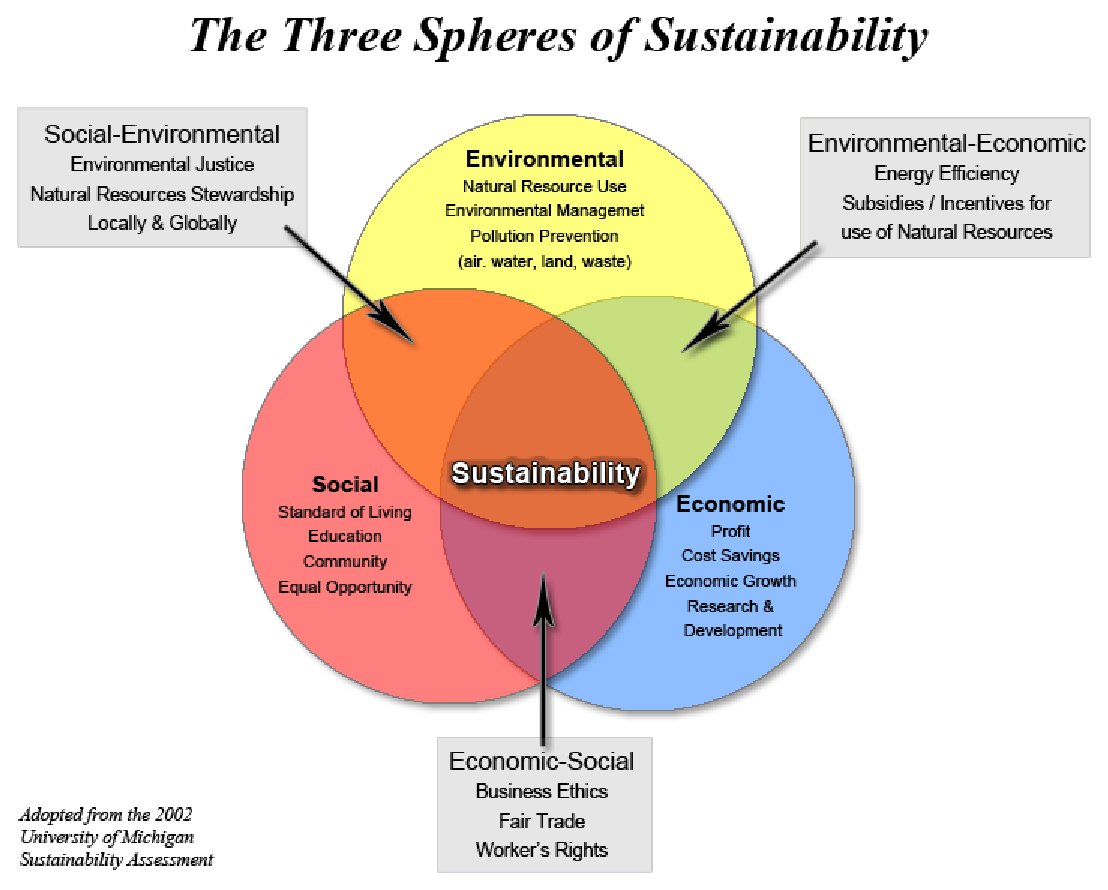
\includegraphics[width=1\columnwidth]{figures/sustainability_spheres}
\par\end{centering}
\caption{Dimensões da sustentabilidade \label{fig:sustainability_spheres}}
\end{figure}

\footnote{Tomada de: http://www.vanderbilt.edu/sustainvu/cms/files/sustainability\_spheres.png}Essas
dimensões serão usadas como contendedores gerais dos conceitos de
sustentabilidade em agricultura permitindo agrupar conceitos relacionados.

\section{Critérios de sustentabilidade}

São variáveis transversais quantitativas e qualitativas, que são monitoradas
regularmente para determinar os efeitos das atividades de intervenção
ou não-intervenção do sistema em avaliação \citet{deusdara2001criterios},
que estabelecem os preceitos de orientação para que os indicadores
sejam representativos para a sustentabilidade.

Cada indicador deverá atender pelo menos um dos critérios de sustentabilidade
para ser considerado um bom indicador de sustentabilidade, os critérios
de sustentabilidade escolhidos pela equipe de especialistas são\citet{moura2002indicadores}:
\begin{itemize}
\item Produtividade: Relacionado a eficiência e custos.
\item Estabilidade: Capacidade do ecossistema de absorver perturbações e
permanecer inalterado (Comissão Econômica para a América Latina e
o Caribe/Programa das Nações Unidas para o Meio Ambiente, CEPAL\nomenclature{CEPAL}{Economic Commission for Latin America and the Caribbean}/PNUMA\nomenclature{PNUMA}{Programa das Nações Unidas para o Meio Ambiente},
1994) 
\item Equidade: Distribuição dos produtos do agroecossistema entre produtores
e consumidores (Dias Junior, 2000) 
\item Resiliência: Capacidade do ecossistema de retornar ao estado original
após de uma perturbação (CEPAL/PNUMA, 1994) 
\item Autonomia: Grau de integração do agroecossistema no fluxo de materiais,
energia e informação entre as partes constituintes e entre o agroecossistema
e o ambiente externo (Fernández, 1995)
\end{itemize}
Esses critérios guiam o desenvolvimento dos conceitos mais relevantes
das metodologias de avaliação de sustentabilidade, os indicadores,
e assim determinar instrumentos de medição que representem os aspectos
críticos do sistema em termos de sustentabilidade.

\section{Atributos Norteadores}

Embora a orientação para a elaboração de todas as variáveis relacionadas
a projetos de sustentabilidade devam atender pelo menos a três pilares:
ambiental, econômico, social, os atributos norteadores são formulados
para garantir as diretrizes no levantamento e validação dos indicadores,
e assim ter um modelo da sustentabilidade dos sistemas de produção
agrícola.

Após a agregação dos dados será possível visualizar as informações
disponíveis e eventuais lacunas para a sistematização dos componentes
dos sistemas produtivos em termos dos requisitos de sustentabilidade.
Em uma primeira instância, devem ser levantados dados referentes ao
solo, clima, água, ar, produção agroindustrial, divisas geradas, mão
de obra envolvida, empregos gerados, doações/benefícios indiretos
à sociedade, biodiversidade, etc.

Uma proposta dos atributos norteadores é a seguinte:
\begin{itemize}
\item Dimensão Ambiental: solo, hídrico, clima, entre outros
\item Dimensão Social: saúde, capacitação, emprego, renda, entre outros
\item Dimensão Econômica: industrial, agrícola, produtividade, custo, entre
outros
\end{itemize}
Os atributos norteadores foram aplicados nos modelos do sistema SustenAgro
como contentores de indicadores os quais classificaram e relacionam
os indicadores em subgrupos das três dimensões da sustentabilidade,
permitindo desta maneira a organização e agrupamento do conhecimento
do domínio.

\section{Método SustenAgro}

Devido à importância da sustentabilidade, especialmente nos sistemas
de produção agrícola, foram desenvolvidas varias métodos para avaliar
o estado desses sistemas, existindo varias tendências segundo o tipo
de sistema produtivo e o contexto deles.

A Embrapa Meio Ambiente coordenou e financiou o projeto SustenAgro
com a finalidade de definir um método de avaliação da sustentabilidade
no sistema produtivo de cana-de-açúcar no centro sul do Brasil, as
características dele são descritas nas figuras \ref{fig:SustenAgro_Description}
e \ref{fig:SustenAgro_Details}, no qual foram originados os indicadores
de sustentabilidade e o método de avaliação \citep{oliveira:2013,BRUMATTI:2015}.

\vfill{}

\pagebreak{}

\begin{figure}[H]
\begin{centering}
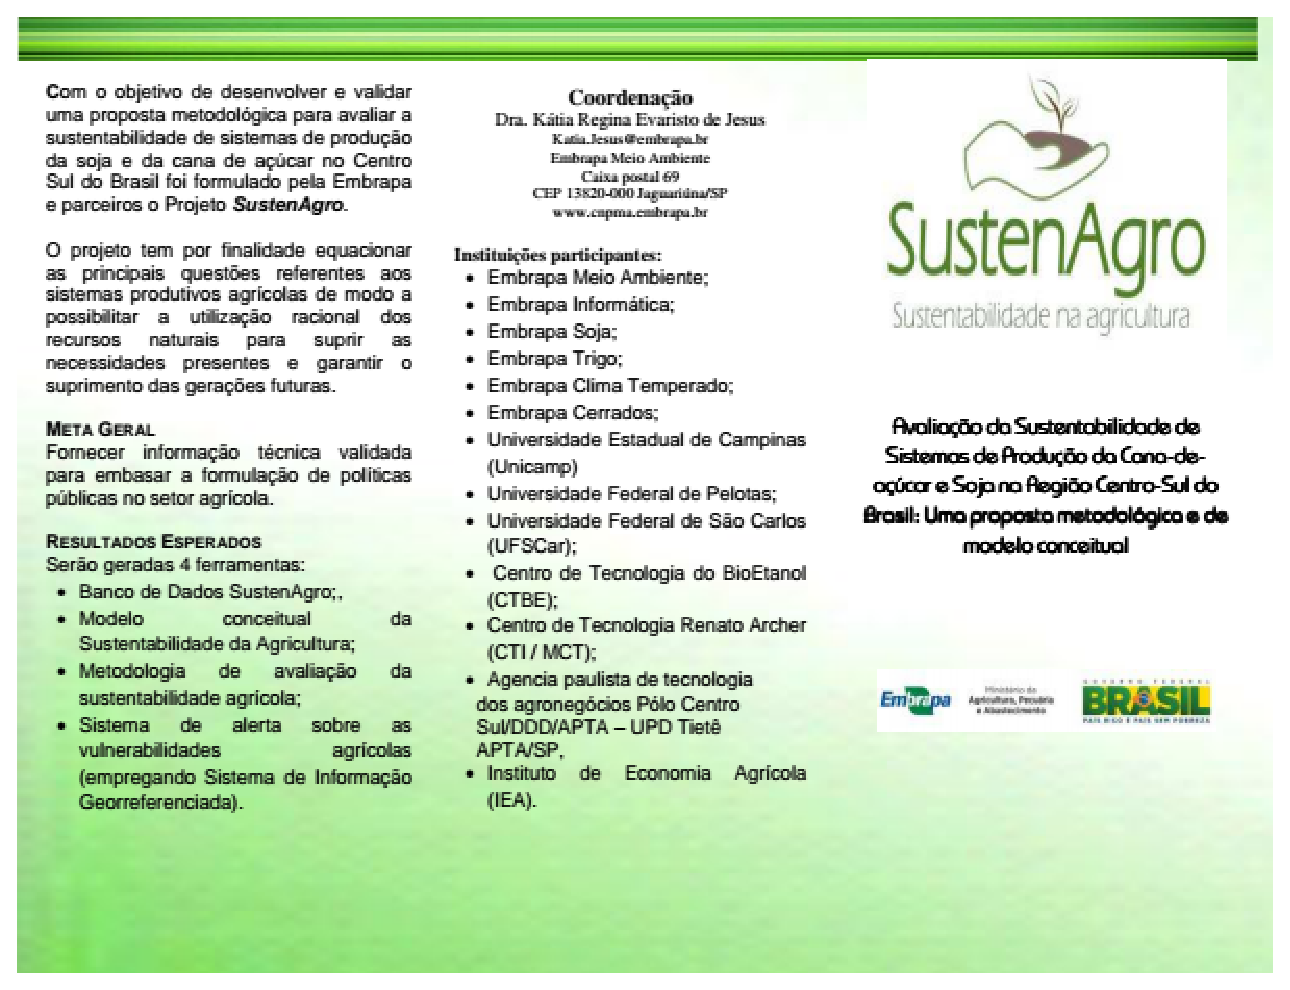
\includegraphics[width=1\columnwidth]{figures/folderEmbrapa1}
\par\end{centering}
\caption{Descrição geral do projeto SustenAgro \label{fig:SustenAgro_Description}}
\end{figure}

\begin{figure}[H]
\begin{centering}
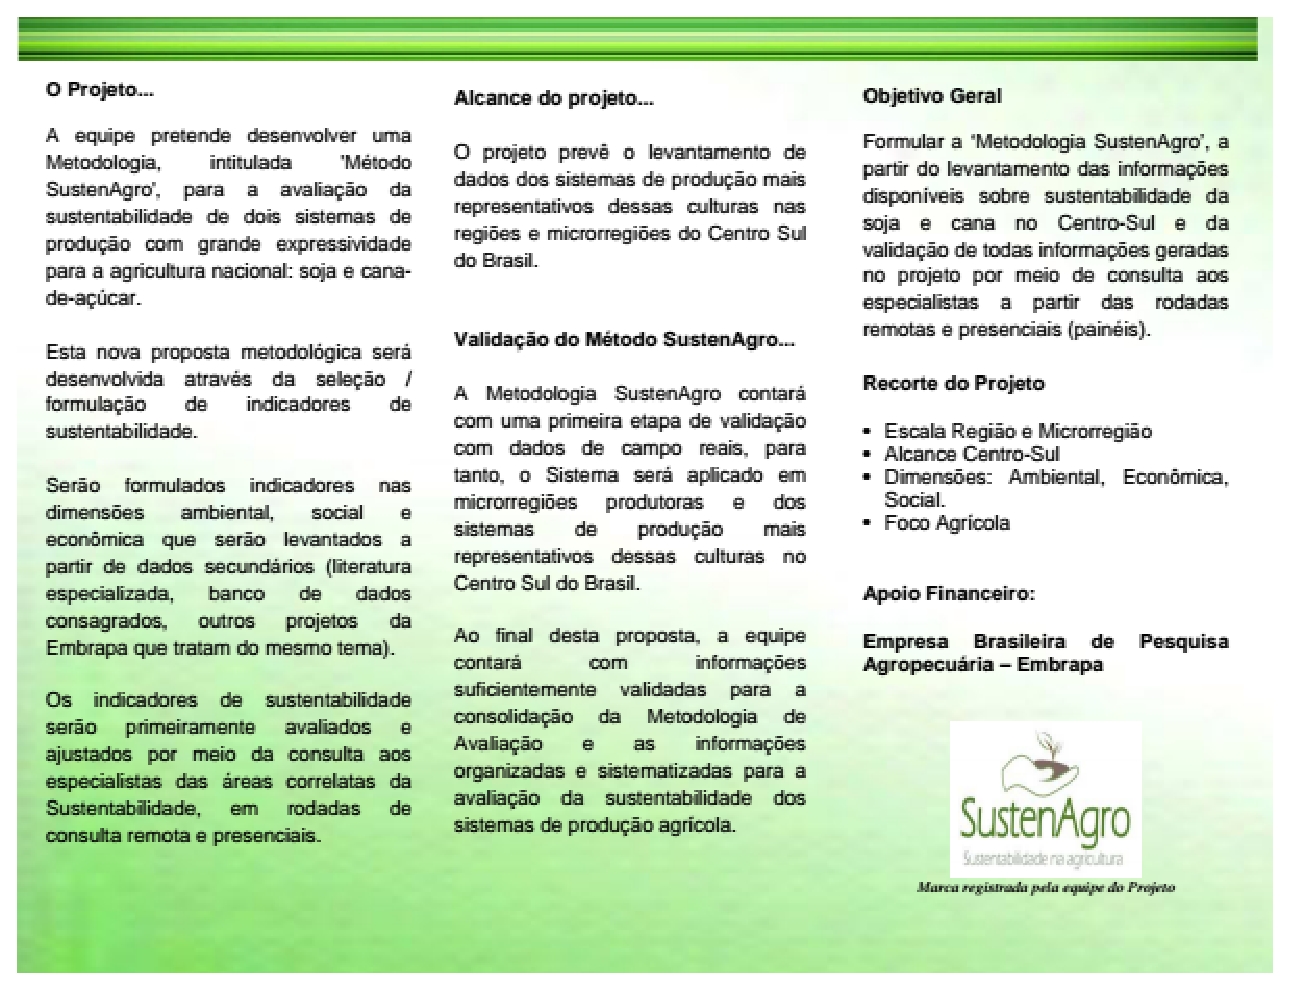
\includegraphics[width=1\columnwidth]{figures/folderEmbrapa2}
\par\end{centering}
\caption{Descrição especifica do projeto SustenAgro \label{fig:SustenAgro_Details}}
\end{figure}

O método SustenAgro foi construído a partir de literatura cientifica
e de instituições de pesquisa como (IBGE\footnote{IBGE: \foreignlanguage{english}{Brazilian Institute of Geography and
Statistics}, \url{http://www.ibge.gov.br/home/}}, CONAB \footnote{CONAB: \foreignlanguage{english}{National Supply Company}, \url{http://www.conab.gov.br/}})
e validados por meio da técnica \foreignlanguage{english}{Delphi}
de consultas aos especialistas.

O método esta composto de dos índices da eficiência e índice da sustentabilidade,
o índice da eficiência esta composto por dois fatores de eficiência
tecnológica no campo e na industria e o índice da sustentabilidade
está composto pelas dimensões ambientais, econômica e social.

\subsection*{Índice de eficiência:}

As equações para calcular o índice da eficiência são:

Formula de eficiência tecnologia no campo:

$efficiency(field)=\sum(CharacteristicsInTheField*RelevanceForTheProductionEnvironment)*correctionFactor(0.8)$

Formula de eficiência tecnologia na industria:

$efficiency(industry)=\sum(CharacteristicsOfProcessing*SugarcaneProcessingOptimization)*correctionFactor(0.2)$

Formula de eficiência produtiva e de costo:

$efficiencyAndCost=\sum(SugarcanEquality+\sum(Logistic+MarketVariables+Policies+Productivity))$

Índice de eficiência:

$EfficiencyIndex=\sum(efficiency(filed)+efficiency(industry))*efficiencyAndCost$

\subsection*{Índice de sustentabilidade}

As equações para calcular o índice de sustentabilidade são:

Formula de eficiência tecnologia no campo:

$EnvironmentalIndex=\sum(EnvironmentalIndicator*EnvironmentIndicatorWeight)$

Formula de eficiência tecnologia na industria:

$EconomicIndex=\sum(EconomicIndicator*EconomicIndicatorWeight)$

Formula de eficiência produtiva e de costo:

$SocialIndex=\sum(SocialIndicator*SocialIndicatorWeight)$

Índice de eficiência:

$SustainabilityIndex=\sum(EnvironmentalIndex+EconomicIndex+SocialIndex)/3$

\section{Matriz de sustentabilidade}

Os índices de eficiência e de sustentabilidade quantificam a sustentabilidade
de uma unidade produtiva, e são representados por meio de uma matriz
que tem como finalidade relacionar o resultado da avaliação com determinadas
classificações correspondentes a cada uns dos quadrantes da matriz,
a figura \ref{fig:Matriz-de-sustentabilidade} representa cada uma
das classificações com os limiares correspondentes a cada índice.

\begin{figure}[h]
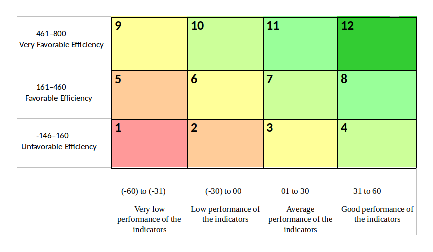
\includegraphics[width=0.8\columnwidth]{figures/SustaiabilityMatrixDesign}

\caption{Matriz de sustentabilidade \label{fig:Matriz-de-sustentabilidade}}

\end{figure}


\section{Conclusões}

O método de avaliação de sustentabilidade foi validado pelos especialistas
e depois de varias iterações definiu-se uma versão estável, que foi
usada no desenvolvimento do Sistema SustenAgro, dito método é mantido
e atualizado pela Embrapa Meio Ambiente e os desenvolvedores de software
garantem que ele se aplique corretamente mas não tem responsabilidade
nenhuma pelas consequências do uso dele.


\chapter{Indicadores de Sustentabilidade}

\label{chap:SustainabilityIndicators}
\section{Índice de Sustentabilidade}

Revela o estado de um sistema ou fenômeno, é uma síntese das características
ou variáveis analisadas. Um índice pode ser construído para analisar
dados através da junção de um jogo de elementos com relacionamentos
estabelecidos. Entende-se o termo índice como um valor numérico que
representa a correta interpretação da realidade de um sistema simples
ou complexo (natural, econômico ou social), utilizando, em seu cálculo,
bases científicas e métodos adequados. O índice pode servir como um
instrumento de tomada de decisão e previsão, e é considerado um nível
superior da junção de um jogo de indicadores ou variáveis \citep{SicheAgostinho2007}

No projeto SustenAgro os índices serão dados numéricos gerais representam
a soma do estado de cada indicador em cada dimensão e atributo norteador,
cada indicador pode o valor de mais um ou menos um (+1 -1), que permitira
quantificar a sustentabilidade em cada aspecto do sistema produtivo
e fazer comparações com outros sistemas produtivos compatíveis.

\section{Limiares de Sustentabilidade}

Os limiares são os pontos mínimo e máximo aceitáveis na amplitude
da sustentabilidade para cada indicador.

Considerando que a sustentabilidade permanece sempre no futuro \citep{gliessman2001agroecologia},
dado o compromisso que os sistemas têm de garantir as necessidades
das gerações futuras, a sustentabilidade será considerada como algo
relativo no espaço e no tempo, ou seja, um sistema pode ser mais ou
menos sustentável do que outro.

Esta representação será realizada pelos limiares de sustentabilidade
que poderão variar de acordo com o sistema de produção considerado
e, principalmente, deve variar de modo a representar com propriedade
das especificidades regionais e microrregionais.

Dentro de uma escala, devem ser estabelecidos limiares críticos, ou
seja, aqueles em que concordamos que determinada situação (característica,
produto, serviço) apesar de não ser totalmente sustentável possui
níveis de sustentabilidade aceitáveis para que a sustentabilidade
seja efetiva (verdadeira), apesar de não ser a ideal. O limiar é um
ponto que estabelece um limite, geralmente é o princípio, mas no nosso
caso, são os limites que apontam que determinada característica, produto,
ou serviço, está dentro do que for considerado sustentabilidade, serão
os pontos mínimo e máximo aceitáveis na amplitude da sustentabilidade.

Dentro desta escala, estabelecemos limiares críticos, ou seja, aqueles
em que concordamos que determinada situação (característica, produto,
serviço) apesar de não ser totalmente sustentável (nota máxima), possui
níveis de sustentabilidade aceitáveis para que a sustentabilidade
seja efetiva (verdadeira), apesar de não ser a ideal. Neste caso,
o limiar mínimo de sustentabilidade assumiria um valor variável.

Exemplo de limiar da sustentabilidade que poderão ser empregados pela
equipe do projeto:
\begin{itemize}
\item Nome do Indicador: Distância Usina / Área de Produção de cana
\item Descrição do indicador: usualmente, em tradicionais regiões produtoras
de cana utiliza-se de uma distância econômica padrão da produção de
50 quilômetros até a indústria. Esta distância é determinada pelos
altos custos de transporte da cana até a unidade industrial, sendo
um dos fatores decisivos na rentabilidade da lavoura (CNA/SENAR, 2007).
\item Limiares de sustentabilidade, teria dois estados possíveis 

\begin{itemize}
\item Distância de até 50 km: Mais sustentável (+1)
\item Distância de mais de 50 km: Menos sustentável (-1)
\end{itemize}
\end{itemize}
Baseando-se nesse conceito sobre limiares é possível desenhar metodologias
de avaliação onde sejam usados os valores numéricos de cada limiar
para fazer comparações, o que permite definir se determinado sistema
produtivo e/ou contexto é mais sustentável do que outro sistema produtivo
e/ou contexto.

\section{Indicadores de Sustentabilidade}

Os indicadores são instrumentos usados para avaliar uma determinada
realidade levando em conta variáveis pertinentes para sua composição.
Além da avaliação, o uso de indicadores permite medir e monitorar
aspectos da realidade. Ele agrega, quantifica e simplifica informações
sobre fenômenos complexos de modo que as tendências ficam mais significativas
e aparentes, a fim de melhorar o processo de entendimento e comunicação\citep{bossel1999indicators,van2005indicadores}.

De acordo com \citep{gallopin1996environmental} os melhores indicadores
são aqueles que simplificam as informações relevantes, tornando os
fenômenos mais claros. Como um indicador é utilizado para atingir
diversos objetivos, é necessário definir um requisito geral para selecionar
indicadores e validar a escolha. A finalidade de um indicador de sustentabilidade
é refletir as alterações nas propriedades fundamentais de um sistema
\citet{CaminoAndMuller1993} e advertir sobre eventuais perturbações
potenciais.\citep{ferraz2003}

Normalmente um indicador é utilizado como um pré-tratamento aos dados
originais \citet{SicheAgostinho2007}. Indicadores são parâmetros
que podem ser utilizados como medida do cumprimento dos critérios
\citep{moret2006criterios}. Deve-se observar que não é possível o
desenvolvimento de um indicador global, por isso é necessário buscar
no tempo a evolução da sustentabilidade dos sistemas \citep{CaminoAndMuller1993}.
Não há indicadores universais, pois eles podem variar segundo o problema
ou objetivo da análise.

Enquanto às características desejáveis para um bom indicador, deve-se
ter uma boa definição da fonte dos dados base para o levantamento,
possibilidade de calibração, possibilidade de comparação com critérios
legais ou outros padrões/metas existentes, facilidade e rapidez de
determinação e interpretação, grau de importância e validação científica,
sensibilidade do público-alvo, custo de implementação e possibilidade
de ser rapidamente atualizado. Nessa mesma linha, \citep{zampieri2003metodo}
baseado em vários autores, cita como requisitos para a seleção de
indicadores de avaliação de sustentabilidade: \renewcommand{\labelenumi}{\roman{enumi}.}
\begin{enumerate}
\item Serem mensuráveis quantitativa e qualitativamente, além de terem pertinência
ao objeto e à natureza do processo avaliado; 
\item Poder coletar as informações por baixo custo, ser de fácil execução
e apresentar dados cientificamente válidos; 
\item Serem concebidos para que o agricultor participe das medições, adaptados
às necessidades dos usuários da informação e estarem embasados em
linguagem clara; 
\item Serem sensíveis às mudanças do sistema ao detectar a magnitude dos
desvios e tendências, oferecendo prognósticos e perspectivas para
planejar e tomar decisões; 
\item Fornecerem indicação clara a respeito da sustentabilidade do sistema
estudado e refletirem os impactos estudados sob o enfoque integrado; 
\item Representarem padrões ecológicos, sociais, econômicos e espaciais,
que tenham correspondência e sensibilidade com o nível de agregação
do sistema considerado; 
\item Conter um nível de agregação que permita comparações individuais,
intertemporais e o cruzamento com outros indicadores; 
\item Fornecerem informações para avaliar os trade-offs entre as dimensões
da sustentabilidade e correlações com os processos dos ecossistemas; 
\item Poder ter repetibilidade, de modo que as medições possam ser realizadas
por diferentes pessoas e que os resultados sejam comparáveis
\item A construção do indicador deve observar parâmetros politicamente corretos.
\end{enumerate}
A OECD (1993) estabelece três requisitos para selecionar indicadores:
relevância política e utilidade para usuários, solidez analítica e
mensurabilidade. 

Alguns exemplos de indicadores levantados no desenvolvimento do método
SustenAgro são: 
\begin{enumerate}
\item Risco climático; 
\item Diversidade de culturas anuais; 
\item Tipo de solo; 
\item Risco de deficit hídrico; 
\item Produtividade da terra; 
\item Renovabilidade energética nos sistemas de produção; 
\item Balanço de nutrientes (nitrogênio e fósforo); 
\item Área de cultivo/áreas preservadas.
\end{enumerate}
Os indicadores do presente projeto são uma representação dos fatores
críticos que existem no sistema de produção de cana-de-açúcar no centro-sul
do Brasil em cada dimensão da sustentabilidade, pelo qual a metodologia
e o sistema SustenAgro é aplicável nesse contexto, no caso de quer
aplicar o sistema de avaliação da sustentabilidade em outro contexto
é necessário mudar os indicadores a cada contexto especifico. 

\section{Dados fornecidos pela Unidade de Meio Ambiente da Embrapa }

A principal fonte de dados para este projeto foi fornecida pela pesquisa
de \citet{oliveira:2013}, onde inicialmente foram identificados 62
indicadores de sustentabilidade no sistema de cana-de-açúcar, os quais
foram analisados e caracterizados, gerando 39 indicadores como os
mais relevantes \citet{BRUMATTI:2015}, por meio de uma validação
com porcentagem maior ou igual a 60\% feita por uma comunidade de
especialistas em sustentabilidade.

A seguintes tabelas mostram os indicadores resultantes, os quais foram
classificados nas três dimensões da sustentabilidade.

Os indicadores da tabela \ref{tab:Indicadores-de-sustentabilidade-ambiental}
representam os valores críticos da dimensão ambiental integrando fenômenos
do solo, dos recursos hídricos e climáticos, os quais permitem caracterizar,
quantificar e comparar o estado da dimensão ambiental de uma unidade
produtiva com outras.

\begin{table}[h]
\begin{tabular}{|>{\raggedright}p{14cm}|}
\hline 
\textbf{Indicadores da dimensão ambiental}\tabularnewline
\hline 
\hline 
Quantificação da erosão potencial segundo a Equação Universal de Perda
de Solo (USLE – \foreignlanguage{english}{Universal Soil Loss Equation})\tabularnewline
\hline 
Compactação do solo\tabularnewline
\hline 
Ocorrência de queimada de palha no campo\tabularnewline
\hline 
Emissão e suspensão de micropartículas (fuligem)\tabularnewline
\hline 
Localização geográfica da cultura em relação à aptidão agroclimática\tabularnewline
\hline 
Localização geográfica da cultura em relação à aptidão edáfica\tabularnewline
\hline 
Localização geográfica da cultura em relação à aptidão edafoclimática\tabularnewline
\hline 
Áreas de Preservação Permanente (APP) recuperadas/conservadas\tabularnewline
\hline 
Comprovação de averbação da área de Reserva Legal\tabularnewline
\hline 
Cumprimento com os Termos de Compromisso de Recuperação Ambiental\tabularnewline
\hline 
\end{tabular}\caption{Indicadores de sustentabilidade de SustenAgro na dimensão ambiental
\label{tab:Indicadores-de-sustentabilidade-ambiental}}
\end{table}

Os indicadores da tabela \ref{tab:Indicadores-de-sustentabilidade-social}
representam os valores críticos da dimensão social integrando fenômenos
de emprego, saúde e treinamento, os quais permitem caracterizar, quantificar
e comparar o estado da dimensão social de uma unidade produtiva com
outras.

\begin{table}[h]
\begin{tabular}{|>{\raggedright}p{14cm}|}
\hline 
\textbf{Indicadores da dimensão social}\tabularnewline
\hline 
\hline 
Poder de compra do trabalhador\tabularnewline
\hline 
\hline 
Taxa de formalidade do emprego\tabularnewline
\hline 
\hline 
Índice Parcial de Educação\tabularnewline
\hline 
\hline 
Índice de internações decorrentes de problemas respiratórios\tabularnewline
\hline 
\hline 
Registro de treinamentos, capacitação ou requalificação de trabalhadores\tabularnewline
\hline 
\end{tabular}

\caption{Indicadores de sustentabilidade de SustenAgro na dimensão social \label{tab:Indicadores-de-sustentabilidade-social} }
\end{table}

Os indicadores da tabela \ref{tab:Indicadores-de-sustentabilidade-economica}
representam os valores críticos da dimensão econômica integrando fenômenos
de emprego, saúde e treinamento, os quais permitem caracterizar, quantificar
e comparar o estado da dimensão social de uma unidade produtiva com
outras.

\begin{table}[h]
\begin{tabular}{|>{\raggedright}p{14cm}|}
\hline 
\textbf{Indicadores da dimensão econômica}\tabularnewline
\hline 
\hline 
\textbf{Indicadores Agrícola/Industrial}\tabularnewline
\hline 
Implantação de biorrefinarias\tabularnewline
\hline 
Rotação de cultura (soja)\tabularnewline
\hline 
Área planta/Área colhida\tabularnewline
\hline 
Atender à Norma Regulamentadora (NR-31)\tabularnewline
\hline 
Longevidade da cana\tabularnewline
\hline 
Distância usina/produção de cana\tabularnewline
\hline 
Controle de pragas favorecidas pela não-queima\tabularnewline
\hline 
Cana queimada manual\tabularnewline
\hline 
Adoção do plantio direto\tabularnewline
\hline 
Predominância da conversão de pastagem em cana-de-açúcar, do que outras
culturas/florestas em cana-de-açúcar\tabularnewline
\hline 
Ocorrência de reutilização de recursos hídricos\tabularnewline
\hline 
Condições favoráveis à mecanização\tabularnewline
\hline 
Otimização do transporte da cana\tabularnewline
\hline 
Consumo de diesel\tabularnewline
\hline 
Variedades melhoradas para condições eco regionais mais específicas\tabularnewline
\hline 
\tabularnewline
\hline 
\textbf{Indicadores Produtos/Subprodutos}\tabularnewline
\hline 
Relação preço gasolina/etanol\tabularnewline
\hline 
Inclusão do Etanol como Commodity\tabularnewline
\hline 
Adoção da tecnologia flex-fuel por outros países\tabularnewline
\hline 
Regulação de comércio de distribuição\tabularnewline
\hline 
Número de contrato para fornecer bioeletricidade\tabularnewline
\hline 
Infraestrutura para a produção de biocombustíveis de 2ª. e 3ª. gerações\tabularnewline
\hline 
\tabularnewline
\hline 
\textbf{Indicadores Tecnológicos}\tabularnewline
\hline 
Desenvolvimento de leveduras mais resistentes a concentrações elevadas
de álcool (Fermentação Extrativa)\tabularnewline
\hline 
\tabularnewline
\hline 
\textbf{Indicadores Políticos}\tabularnewline
\hline 
Iniciativas do poder público com a proteção ao ambiente\tabularnewline
\hline 
\end{tabular}

\caption{Indicadores de sustentabilidade de SustenAgro na dimensão econômica\label{tab:Indicadores-de-sustentabilidade-economica}}
\end{table}

Cada um dos anteriores indicadores foram definidos com um conjunto
de pelo menos um componente de indicador, estes componentes permitem
quantificar por meio de uma variável quantitativa o estado do indicador,
os quais estão definidos em termos do domínio que são de fácil interpretação
pelas pessoas relacionadas com sustentabilidade em agricultura.

\section{Considerações finais}

Os dados e especificações fornecidos pela Embrapa Meio Ambiente e
pela APTA conseguiram explicar o conceito de avaliação de sustentabilidade
segundo a visão da Embrapa Meio Ambiente, más a complexidade envolvida
requereu identificar um tipo de KOS que permita representar cada uns
dos conceitos necessários que compõem o processo de avaliação da sustentabilidade.

Dito KOS precisa ser flexível e de fácil uso para conseguir se adaptar
às mudanças do domínio, devido a que durante o processo de modelagem
avalia a coerência dos dados, permitindo assim melhorar as especificações
de dito domínio.


\chapter{Instalação}

\label{chap:Instalation}A instalação dos Sistemas Decisioner e SustenAgro divide-se em dois
processos, a configuração do servidor web e o deploy do arquivo WAR\nomenclature{WAR}{Web Application Archive},
a continuação são descritos ambos processos:

\section{Configuração do servidor.}

Esta fase do processo consiste em instalar as tecnologias Java, Apache
Tomcat, WkHtmltoPdf e a triplestore Blazegraph, em um servidor baseado
em linux, atualmente o sistema foi configurado e testado em uma maquina
virtual com Ubuntu 14.04, Java OpenJDK 8, Apache Tomcat, WkHtmltoPdf
0.12.3 e a triplestore Blazegraph 2.1.0, a instalação destas tecnologias
segue uma orientação padrão que sera descrita a continuação:

\subsection{Instalação do Java:}

Segundo a documentação de Java OpenJDK, a instalação é realizada por
meio do comando:

\inputencoding{latin9}\begin{lstlisting}
sudo apt-get update
sudo apt-get install openjdk-8-jre
\end{lstlisting}
\inputencoding{utf8}

\subsection{Instalação do Apache Tomcat}

A instalação do Apache Tomcat depende da instalação do Java 8, e o
Tomcat versão 7 para suportar a compatibilidade do War gerado, isto
é documentado no site\footnote{https://grails.org/wiki/Deployment}
do framework Grails, que exige uma versão 7 de Apache Tomcat para
suportar o deploy dos arquivos war.

O processo de instalação consiste em fazer download dos arquivos binários,
extrair eles em /opt/tomcat/, exportar as variáveis de entorno e executar
o Web Server, o código é mostrado a continuação:

\inputencoding{latin9}\begin{lstlisting}
wget http://www-eu.apache.org/dist/tomcat/tomcat-7/v7.0.70/bin/
apache-tomcat-7.0.70.tar.gz

tar xvzf apache-tomcat-7.0.70.tar.gz -C /opt/tomcat

sudo /opt/tomcat/bin/startup.sh
\end{lstlisting}
\inputencoding{utf8}
Configurar users de Tomcat em: /opt/tomcat/conf/tomcat-users.xml e
acrescentar os Rol e User

\inputencoding{latin9}\begin{lstlisting}
<role rolename="manager-gui"/> 
<user username="admin" password="s3cr3t" roles="manager-gui"/>
\end{lstlisting}
\inputencoding{utf8}
Depois disso, é registrado no final do arquivo \textasciitilde{}/.bashrc
os próximos dois comandos que definem as variáveis de entorno

\inputencoding{latin9}\begin{lstlisting}
export JAVA_HOME=/usr/lib/jvm/java-1.8.0-openjdk-amd64 
export CATALINA_HOME=/opt/tomcat
\end{lstlisting}
\inputencoding{utf8}
Finalmente executar o comando 

\inputencoding{latin9}\begin{lstlisting}
sudo /opt/tomcat/bin/startup.sh
\end{lstlisting}
\inputencoding{utf8}
e verificar a execução do programa na url /manager do domínio do servidor

\subsection{Instalação do WkHtmltoPdf}

A tecnologia WkHtmltoPdf permite converter paginas web em formato
Html a Pdf, esta ferramenta suporta a funcionalidade de gerar os reportes
em formato Pdf, a instalação consistem em fazer download dos arquivos
binários e a configuração de um X Server Virual para suportar o renderizado,
os comandos são mostrados a continuação:

\inputencoding{latin9}\begin{lstlisting}
wget http://download.gna.org/wkhtmltopdf/0.12/0.12.3/
wkhtmltox-0.12.3_linux-generic-amd64.tar.xz

tar xf wkhtmltox-0.12.3_linux-generic-amd64.tar.xz

cp wkhtmltox/bin/wkhtmltopdf /usr/local/bin/wkhtmltopdf

sudo chmod a+x /usr/local/bin/wkhtmltopdf

sudo apt-get install openssl build-essential xorg libssl-dev
\end{lstlisting}
\inputencoding{utf8}
Depois disto é criado um script wkhtmltopdf.sh em /usr/local/bin/
e contem o seguinte comando:

\inputencoding{latin9}\begin{lstlisting}
xvfb-run -a -s "-screen 0 640x480x16" wkhtmltopdf "$@"
sudo chmod a+x /usr/local/bin/wkhtmltopdf.sh 
\end{lstlisting}
\inputencoding{utf8}
Com o comando wkhtmltopdf.sh é possível converter a pdf desde um sistema
sem X11

\subsubsection*{Instalação da Triplestore Blazegraph}

A instalação do Blazegraph consiste em fazer download do arquivo binário
e executar com o arquivo de configuração RWStore2.properties o serviço
de triplestore.

\inputencoding{latin9}\begin{lstlisting}
wget https://sourceforge.net/projects/bigdata/files/bigdata/
2.1.1/blazegraph.jar

wget https://dl.dropboxusercontent.com/u/24827919/
SustenAgro/RWStore2.properties

java -server -Xmx4g -Dbigdata.propertyFile=RWStore2.properties 
-jar blazegraph.jar
\end{lstlisting}
\inputencoding{utf8}

\section{Deploy do arquivo war}

O deploy do sistema consiste em executar os serviços do Tomcat 7 e
Triplestore, e fazer upload do arquivo SustenAgro-1.0.war ao servidor
Apache Tomcat para fazer o deploy no Path ``/'', e finalmente reiniciar
o Tomcat.

\inputencoding{latin9}\begin{lstlisting}
wget https://dl.dropboxusercontent.com/u/24827919/
SustenAgro/sustenagro-1.0.war
\end{lstlisting}
\inputencoding{utf8}


\chapter{Formulários de avaliação\label{chap:formularios}}


\section{Formulário de avaliação SustenAgro\label{sec:Formul=0000E1rio-de-avalia=0000E7=0000E3o-SustenAgro}}

O processo consiste em realizar cinco tarefas descritas a continuação,
e responder as seguintes três perguntas para cada tarefa: 
\begin{itemize}
\item Conseguiu realizar a tarefa?
\item Teve algum problema/dúvida durante a realização da tarefa?
\item Tem sugestões que permitam melhorar/facilitar a realização da tarefa?
\end{itemize}

\subsection*{Tarefa 1}

Cadastrar usuário:
\begin{enumerate}
\item Ingressar no software SustenAgro em http://java.icmc.usp.br:1300/
\item Dar click na opção de 'Inscrever-se' e ingressar no formulário de
cadastro de novo usuário
\item Preencher o formulário e enviar
\item Ingressar ao sistema com seus dados cadastrados. 
\end{enumerate}

\subsection*{Tarefa 2}

Cadastrar uma unidade produtiva: 
\begin{enumerate}
\item Dar click no link de 'Avaliação'
\item Cadastrar no formulário de uma nova unidade produtiva.
\item Preencher o formulário e enviar 
\end{enumerate}

\subsection*{Tarefa 3}

Preencher dados da avaliação: 

Se a anterior tarefa foi realizada com sucesso, o sistema vai encaminhá-lo
ao formulário de nova avaliação, em caso negativo pode dar click no
botão 'Análises' e 'Nova Análise', para realizar:
\begin{enumerate}
\item Preencher alguns dados de avaliação de eficiência e custo
\item Preencher alguns dados de avaliação da sustentabilidade
\item Solicitar avaliação por meio do botão 'Avaliar' 
\end{enumerate}

\subsection*{Tarefa 4}

Visualizar os resultados: 

Se a anterior tarefa foi realizada com sucesso, o sistema vai encaminhá-lo
a tela de 'Resultados da avaliação', em caso negativo pode dar click
no botão 'Análises' e selecionar a análise cadastrada, para realizar:
\begin{enumerate}
\item Visualizar a planilha de eficiência e custo
\item Visualizar a planilha de sustentabilidade
\item Visualizar o relatório da avaliação
\item Visualizar os dados da avaliação na aba 'Avaliação'
\end{enumerate}

\subsection*{Tarefa 5}

Editar avaliação: 
\begin{enumerate}
\item Na tela de 'Resultados da avaliação' selecionar a aba 'Avaliação'
\item Acrescentar alguns dados de avaliação de eficiência e custo
\item Acrescentar alguns dados de avaliação da sustentabilidade
\item Solicitar a atualização por meio do botão 'Atualizar' 
\end{enumerate}

\section{Formulário de avaliação Decisioner\label{sec:Formul=0000E1rio-de-avalia=0000E7=0000E3o-Decisioner}}

O processo consiste em realizar cinco tarefas descritas a seguir,
e responder as seguintes três perguntas para cada tarefa:
\begin{itemize}
\item Conseguiu realizar a tarefa?
\item Teve algum problema/dúvida durante a realização da tarefa?
\item Tem sugestões para melhorar/facilitar a realização da tarefa?
\end{itemize}
As seguintes tarefas devem ser realizadas na interface de administração
do sistema:

\subsection*{Tarefa 1}

Cadastrar novo indicador
\begin{enumerate}
\item Ingressar com login de administrador no software SustenAgro em http://java.icmc.usp.br:1300/
\item Dar click no link 'Ontology'
\item Clicar em Feature, Indicador, Indicador de Sustentabilidade e Dimensão
Social
\item Cadastrar uma nova dimensão, atributo e indicador a partir da linha
1020 no seguinte formato:\inputencoding{latin9}
\begin{lstlisting}[caption={Codigo de novo indicador}]
AgriculturalIndicator: 
 is_a: SustainabilityIndicator 
 relevance: 1.0 
 label: 
  - Agricultural dimension @en 
  - Dimens�o agricultural @pt

DeforestationAttribute: 
 is_a: AgriculturalIndicator 
 label: 
  - Atributo desmatamento @pt 
  - Deforestation attribute @en 

DeforestationIndicator: 
 is_a: DeforestationAttribute 
 label: 
  - Indicador desmatamento @pt 
  - Deforestation indicator @en 
 relevance: 2.0 
 value: YesNo
\end{lstlisting}
\inputencoding{utf8}\item Dar click na opção “Save”
\item Acrescentar a nova dimensão na DSL, clicando na Aba DSL e no link
Main adicionar na linha 106 o seguinte código\inputencoding{latin9}
\begin{lstlisting}[caption={Adi��o de feature na DSL}]
feature ':AgriculturalIndicator'
\end{lstlisting}
\inputencoding{utf8}\item Dar click na opção “Save” - Procurar o indicador cadastrado na interface
de Usuário, na tela de Usuário na aba Avaliação selecionar uma Unidade
Produtiva e ir em Nova Avaliação
\end{enumerate}

\subsection*{Tarefa 2}

Editar a formula de avaliação 
\begin{enumerate}
\item Dar click no link 'DSL'
\item Procurar o comando Report e editar algum valor da fórmula
\item Dar click na opção “Save”
\item Visualizar os índices de uma avaliação cadastrada no sistema por meio
da aba Report, na tela de Usuário na aba Avaliação selecionar uma
Unidade Produtiva, selecionar uma Avaliação e um Report ligado a ela
\end{enumerate}

\subsection*{Tarefa 3}

Editar os limiares das widgets matriz e semáforo de avaliação
\begin{enumerate}
\item Dar click no link 'DSL'
\item Procurar o comando sustainabilityMatrix e editar o valor de range\_x
\item Procurar o comando sustainabilitySemaphore e editar o valor de range
\item Dar click na opção “Save”
\item Visualizar os índices de uma avaliação cadastrada no sistema, na tela
de Usuário na aba Avaliação selecionar uma Unidade Produtiva, selecionar
uma Avaliação e um Report ligado a ela
\end{enumerate}

\subsection*{Tarefa 4}

Editar uma View
\begin{enumerate}
\item Dar click no link 'Views'
\item Selecionar uma a view de contact
\item Editar o título da view por meio do comando pageHeader
\item Dar click na opção “Save”
\item Visualizar a view na interface do Usuário por meio do link Contact
\end{enumerate}

\subsection*{Tarefa 5}

Editar labels das internationalizations
\begin{enumerate}
\item Dar click no link 'Internationalization'
\item Seleccionar ingles
\item Editar o texto de um label
\item Dar click na opção “Save”
\item Visualizar uma view que faça uso do label editado na interface do
Usuário
\end{enumerate}

\section{Formulário Delphi para Workshop SustenAgro\label{sec:Formulario-Delphi-Workshop}}

\includepdf[pages=-,width=1\columnwidth]{/home/john/Desktop/Dissertation/pages/workshop}


\end{document}
